%% Ngân hàng đề Toán 12 (KNTT) -- Chương I, Bài 4, Dạng 04
%% Dạng: Số nghiệm của phương trình, sự tương giao của các đồ thị
%% Phương án ĐẦU TIÊN trong \cauTN luôn là đáp án đúng (gói trondethi tự đảo).
%% Phần II: \y{nội dung}{d|s}. Phần III: đáp án đặt ở đối số cuối.

\cauTN[id=C1-B4-D04-NB-001,muc=NB,loigiai={Phương trình hoành độ giao điểm: $-x^{3}-6x^{2}-13x-9=-2x-3\Leftrightarrow -x^{3}-6x^{2}-11x-6=0\Leftrightarrow x=-3 \vee x=-2 \vee x=-1$. Các giao điểm: $(-3;3)$, $(-2;1)$, $(-1;-1)$.}]{Cho hàm số $y=-x^{3}-6x^{2}-13x-9$ có đồ thị $(C)$ và đường thẳng $d: y=-2x-3$. Số giao điểm của $(C)$ và $d$ là}
  {$3$.}
  {$2$.}{$1$.}{$0$.}

\cauTN[id=C1-B4-D04-NB-002,muc=NB,loigiai={Phương trình hoành độ giao điểm: $x^{3}-3x^{2}-5x+10=-x-2\Leftrightarrow x^{3}-3x^{2}-4x+12=0\Leftrightarrow x=-2 \vee x=2 \vee x=3$. Các giao điểm: $(-2;0)$, $(2;-4)$, $(3;-5)$.}]{Cho hàm số $y=x^{3}-3x^{2}-5x+10$ có đồ thị $(C)$ và đường thẳng $d: y=-x-2$. Tổng hoành độ các giao điểm của $(C)$ và $d$ bằng}
  {$3$.}
  {$5$.}{$1$.}{$2$.}

\cauTN[id=C1-B4-D04-NB-003,muc=NB,loigiai={Phương trình hoành độ giao điểm: $-x^{3}-5x^{2}-6x-4=2x\Leftrightarrow -x^{3}-5x^{2}-8x-4=0\Leftrightarrow x=-2 \vee x=-1$. Các giao điểm: $(-2;-4)$, $(-1;-2)$.}]{Cho hàm số $y=-x^{3}-5x^{2}-6x-4$ có đồ thị $(C)$ và đường thẳng $d: y=2x$. Điểm nào dưới đây là một giao điểm của $(C)$ và $d$?}
  {$(-1;-2)$.}
  {$(-2;-1)$.}{$(-1;-1)$.}{$(1;-2)$.}

\cauTN[id=C1-B4-D04-NB-004,muc=NB,loigiai={Phương trình hoành độ giao điểm: $-x^{3}+3x^{2}+x+1=x+1\Leftrightarrow -x^{3}+3x^{2}=0\Leftrightarrow x=0 \vee x=3$. Các giao điểm: $(0;1)$, $(3;4)$.}]{Cho hàm số $y=-x^{3}+3x^{2}+x+1$ có đồ thị $(C)$ và đường thẳng $d: y=x+1$. Số giao điểm của $(C)$ và $d$ là}
  {$2$.}
  {$3$.}{$1$.}{$0$.}

\cauTN[id=C1-B4-D04-NB-005,muc=NB,loigiai={Phương trình hoành độ giao điểm: $x^{3}-x-4=2x-2\Leftrightarrow x^{3}-3x-2=0\Leftrightarrow x=-1 \vee x=2$. Các giao điểm: $(-1;-4)$, $(2;2)$.}]{Cho hàm số $y=x^{3}-x-4$ có đồ thị $(C)$ và đường thẳng $d: y=2x-2$. Số giao điểm của $(C)$ và $d$ là}
  {$2$.}
  {$3$.}{$1$.}{$0$.}

\cauTN[id=C1-B4-D04-NB-006,muc=NB,loigiai={Phương trình hoành độ giao điểm: $-x^{3}-7x^{2}-14x-10=x-1\Leftrightarrow -x^{3}-7x^{2}-15x-9=0\Leftrightarrow x=-3 \vee x=-1$. Các giao điểm: $(-3;-4)$, $(-1;-2)$.}]{Cho hàm số $y=-x^{3}-7x^{2}-14x-10$ có đồ thị $(C)$ và đường thẳng $d: y=x-1$. Số giao điểm của $(C)$ và $d$ là}
  {$2$.}
  {$3$.}{$1$.}{$0$.}

\cauTN[id=C1-B4-D04-NB-007,muc=NB,loigiai={Phương trình hoành độ giao điểm: $x^{3}+5x^{2}+5x=-x\Leftrightarrow x^{3}+5x^{2}+6x=0\Leftrightarrow x=-3 \vee x=-2 \vee x=0$. Các giao điểm: $(-3;3)$, $(-2;2)$, $(0;0)$.}]{Cho hàm số $y=x^{3}+5x^{2}+5x$ có đồ thị $(C)$ và đường thẳng $d: y=-x$. Số giao điểm của $(C)$ và $d$ là}
  {$3$.}
  {$2$.}{$1$.}{$0$.}

\cauTN[id=C1-B4-D04-NB-008,muc=NB,loigiai={Phương trình hoành độ giao điểm: $x^{3}-4x^{2}+3x+2=2\Leftrightarrow x^{3}-4x^{2}+3x=0\Leftrightarrow x=0 \vee x=1 \vee x=3$. Các giao điểm: $(0;2)$, $(1;2)$, $(3;2)$.}]{Cho hàm số $y=x^{3}-4x^{2}+3x+2$ có đồ thị $(C)$ và đường thẳng $d: y=2$. Số giao điểm của $(C)$ và $d$ là}
  {$3$.}
  {$2$.}{$1$.}{$0$.}

\cauTN[id=C1-B4-D04-NB-009,muc=NB,loigiai={Phương trình hoành độ giao điểm: $x^{3}+5x^{2}+10x+1=2x-3\Leftrightarrow x^{3}+5x^{2}+8x+4=0\Leftrightarrow x=-2 \vee x=-1$. Các giao điểm: $(-2;-7)$, $(-1;-5)$.}]{Cho hàm số $y=x^{3}+5x^{2}+10x+1$ có đồ thị $(C)$ và đường thẳng $d: y=2x-3$. Số giao điểm của $(C)$ và $d$ là}
  {$2$.}
  {$3$.}{$1$.}{$0$.}

\cauTN[id=C1-B4-D04-NB-010,muc=NB,loigiai={Phương trình hoành độ giao điểm: $-x^{3}-6x^{2}-12x-4=-x+2\Leftrightarrow -x^{3}-6x^{2}-11x-6=0\Leftrightarrow x=-3 \vee x=-2 \vee x=-1$. Các giao điểm: $(-3;5)$, $(-2;4)$, $(-1;3)$.}]{Cho hàm số $y=-x^{3}-6x^{2}-12x-4$ có đồ thị $(C)$ và đường thẳng $d: y=-x+2$. Tổng hoành độ các giao điểm của $(C)$ và $d$ bằng}
  {$-6$.}
  {$-3$.}{$6$.}{$-5$.}

\cauTN[id=C1-B4-D04-NB-011,muc=NB,loigiai={Số nghiệm của phương trình $f(x)=-7$ bằng số giao điểm của đồ thị $y=f(x)$ với đường thẳng $y=-7$. Dựa vào đồ thị ta được $1$ nghiệm.}]{Cho hàm số $y=f(x)$ có đồ thị như hình vẽ.
\begin{center}
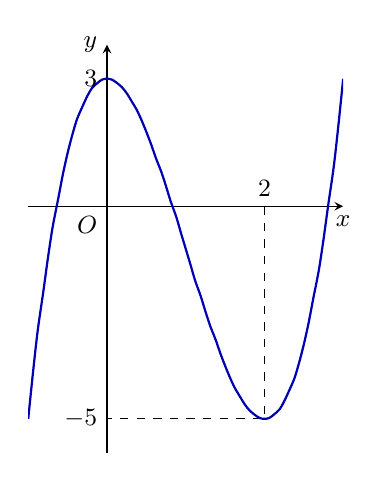
\begin{tikzpicture}[x=1cm,y=0.54cm,>=stealth,font=\small]
\draw[->] (-1,0)--(3,0) node[below]{$x$};
\draw[->] (0,-5.8)--(0,3.8) node[left]{$y$};
\node[below left] at (0,0){$O$};
\draw[dashed,thin] (2,0)--(2,-5)--(0,-5);
\begin{scope}\clip (-1,-5.81) rectangle (3,3.8);
\draw[thick,blue!70!black] plot[smooth] coordinates {(-1,-5) (-0.94,-3.92) (-0.88,-2.93) (-0.81,-2.03) (-0.75,-1.22) (-0.69,-0.49) (-0.62,0.17) (-0.56,0.75) (-0.5,1.25) (-0.44,1.68) (-0.38,2.05) (-0.31,2.35) (-0.25,2.59) (-0.19,2.78) (-0.12,2.9) (-0.06,2.98) (0,3) (0.06,2.98) (0.12,2.91) (0.19,2.8) (0.25,2.66) (0.31,2.48) (0.38,2.26) (0.44,2.02) (0.5,1.75) (0.56,1.46) (0.62,1.14) (0.69,0.81) (0.75,0.47) (0.81,0.11) (0.88,-0.25) (0.94,-0.63) (1,-1) (1.06,-1.37) (1.12,-1.75) (1.19,-2.11) (1.25,-2.47) (1.31,-2.81) (1.38,-3.14) (1.44,-3.46) (1.5,-3.75) (1.56,-4.02) (1.62,-4.26) (1.69,-4.48) (1.75,-4.66) (1.81,-4.8) (1.88,-4.91) (1.94,-4.98) (2,-5) (2.06,-4.98) (2.12,-4.9) (2.19,-4.78) (2.25,-4.59) (2.31,-4.35) (2.38,-4.05) (2.44,-3.68) (2.5,-3.25) (2.56,-2.75) (2.62,-2.17) (2.69,-1.51) (2.75,-0.78) (2.81,0.03) (2.88,0.93) (2.94,1.92) (3,3)};
\end{scope}
\node[above] at (2,0){$2$};
\node[left] at (0,-5){$-5$};
\node[left] at (0,3){$3$};
\end{tikzpicture}
\end{center}
Số nghiệm thực của phương trình $f(x)=-7$ là}
  {$1$.}
  {$2$.}{$0$.}{$3$.}

\cauTN[id=C1-B4-D04-NB-012,muc=NB,loigiai={Phương trình hoành độ giao điểm: $x^{3}-5x^{2}+4x+8=x-1\Leftrightarrow x^{3}-5x^{2}+3x+9=0\Leftrightarrow x=-1 \vee x=3$. Các giao điểm: $(-1;-2)$, $(3;2)$.}]{Cho hàm số $y=x^{3}-5x^{2}+4x+8$ có đồ thị $(C)$ và đường thẳng $d: y=x-1$. Số giao điểm của $(C)$ và $d$ là}
  {$2$.}
  {$3$.}{$1$.}{$0$.}

\cauTN[id=C1-B4-D04-NB-013,muc=NB,loigiai={Phương trình hoành độ giao điểm: $-x^{3}+x^{2}+6x-1=2x+3\Leftrightarrow -x^{3}+x^{2}+4x-4=0\Leftrightarrow x=-2 \vee x=1 \vee x=2$. Các giao điểm: $(-2;-1)$, $(1;5)$, $(2;7)$.}]{Cho hàm số $y=-x^{3}+x^{2}+6x-1$ có đồ thị $(C)$ và đường thẳng $d: y=2x+3$. Tổng hoành độ các giao điểm của $(C)$ và $d$ bằng}
  {$1$.}
  {$3$.}{$5$.}{$2$.}

\cauTN[id=C1-B4-D04-NB-014,muc=NB,loigiai={Phương trình hoành độ giao điểm: $-x^{3}-x^{2}+10x+10=x+1\Leftrightarrow -x^{3}-x^{2}+9x+9=0\Leftrightarrow x=-3 \vee x=-1 \vee x=3$. Các giao điểm: $(-3;-2)$, $(-1;0)$, $(3;4)$.}]{Cho hàm số $y=-x^{3}-x^{2}+10x+10$ có đồ thị $(C)$ và đường thẳng $d: y=x+1$. Số giao điểm của $(C)$ và $d$ là}
  {$3$.}
  {$2$.}{$1$.}{$0$.}

\cauTN[id=C1-B4-D04-NB-015,muc=NB,loigiai={Số nghiệm của phương trình $f(x)=3$ bằng số giao điểm của đồ thị $y=f(x)$ với đường thẳng $y=3$. Dựa vào đồ thị ta được $1$ nghiệm.}]{Cho hàm số $y=f(x)$ có đồ thị như hình vẽ.
\begin{center}
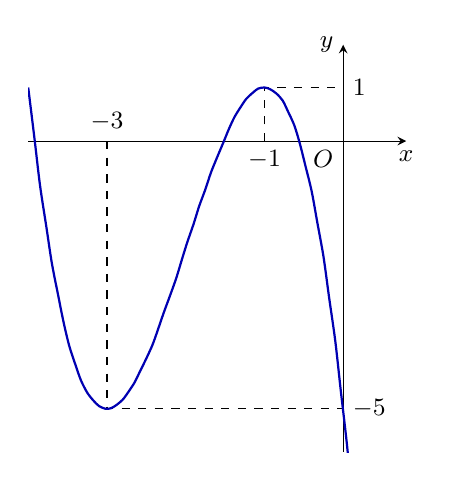
\begin{tikzpicture}[x=1cm,y=0.68cm,>=stealth,font=\small]
\draw[->] (-4,0)--(0.8,0) node[below]{$x$};
\draw[->] (0,-5.8)--(0,1.8) node[left]{$y$};
\node[below left] at (0,0){$O$};
\draw[dashed,thin] (-3,0)--(-3,-5)--(0,-5);
\draw[dashed,thin] (-1,0)--(-1,1)--(0,1);
\begin{scope}\clip (-4,-5.81) rectangle (0.8,1.8);
\draw[thick,blue!70!black] plot[smooth] coordinates {(-4,1) (-3.92,0.04) (-3.85,-0.83) (-3.77,-1.6) (-3.7,-2.28) (-3.62,-2.88) (-3.55,-3.39) (-3.48,-3.82) (-3.4,-4.18) (-3.33,-4.47) (-3.25,-4.7) (-3.17,-4.85) (-3.1,-4.95) (-3.02,-5) (-2.95,-4.99) (-2.88,-4.93) (-2.8,-4.83) (-2.73,-4.69) (-2.65,-4.51) (-2.58,-4.3) (-2.5,-4.06) (-2.42,-3.8) (-2.35,-3.51) (-2.28,-3.21) (-2.2,-2.89) (-2.12,-2.56) (-2.05,-2.22) (-1.98,-1.89) (-1.9,-1.55) (-1.83,-1.22) (-1.75,-0.9) (-1.68,-0.59) (-1.6,-0.3) (-1.52,-0.02) (-1.45,0.23) (-1.38,0.45) (-1.3,0.64) (-1.23,0.79) (-1.15,0.9) (-1.08,0.98) (-1,1) (-0.93,0.97) (-0.85,0.89) (-0.77,0.76) (-0.7,0.55) (-0.62,0.29) (-0.55,-0.05) (-0.48,-0.46) (-0.4,-0.94) (-0.33,-1.51) (-0.25,-2.16) (-0.18,-2.91) (-0.1,-3.74) (-0.03,-4.67) (0.05,-5.7) (0.12,-6.83) (0.2,-8.07) (0.27,-8.8) (0.35,-8.8) (0.42,-8.8) (0.5,-8.8) (0.58,-8.8) (0.65,-8.8) (0.72,-8.8) (0.8,-8.8)};
\end{scope}
\node[above] at (-3,0){$-3$};
\node[below] at (-1,0){$-1$};
\node[right] at (0,-5){$-5$};
\node[right] at (0,1){$1$};
\end{tikzpicture}
\end{center}
Số nghiệm thực của phương trình $f(x)=3$ là}
  {$1$.}
  {$2$.}{$0$.}{$3$.}

\cauTN[id=C1-B4-D04-NB-016,muc=NB,loigiai={Phương trình hoành độ giao điểm: $-x^{3}+x^{2}-x+2=-2x+3\Leftrightarrow -x^{3}+x^{2}+x-1=0\Leftrightarrow x=-1 \vee x=1$. Các giao điểm: $(-1;5)$, $(1;1)$.}]{Cho hàm số $y=-x^{3}+x^{2}-x+2$ có đồ thị $(C)$ và đường thẳng $d: y=-2x+3$. Số giao điểm của $(C)$ và $d$ là}
  {$2$.}
  {$3$.}{$1$.}{$0$.}

\cauTN[id=C1-B4-D04-NB-017,muc=NB,loigiai={Số nghiệm của phương trình $f(x)=-5$ bằng số giao điểm của đồ thị $y=f(x)$ với đường thẳng $y=-5$. Dựa vào đồ thị ta được $2$ nghiệm.}]{Cho hàm số $y=f(x)$ có đồ thị như hình vẽ.
\begin{center}
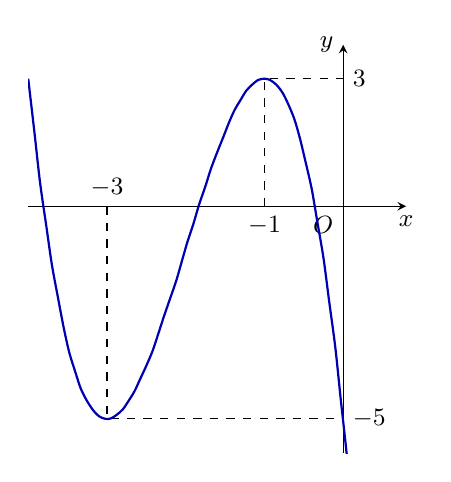
\begin{tikzpicture}[x=1cm,y=0.54cm,>=stealth,font=\small]
\draw[->] (-4,0)--(0.8,0) node[below]{$x$};
\draw[->] (0,-5.8)--(0,3.8) node[left]{$y$};
\node[below left] at (0,0){$O$};
\draw[dashed,thin] (-3,0)--(-3,-5)--(0,-5);
\draw[dashed,thin] (-1,0)--(-1,3)--(0,3);
\begin{scope}\clip (-4,-5.81) rectangle (0.8,3.8);
\draw[thick,blue!70!black] plot[smooth] coordinates {(-4,3) (-3.92,1.72) (-3.85,0.56) (-3.77,-0.47) (-3.7,-1.37) (-3.62,-2.17) (-3.55,-2.85) (-3.48,-3.43) (-3.4,-3.91) (-3.33,-4.3) (-3.25,-4.59) (-3.17,-4.81) (-3.1,-4.94) (-3.02,-5) (-2.95,-4.99) (-2.88,-4.91) (-2.8,-4.78) (-2.73,-4.59) (-2.65,-4.35) (-2.58,-4.07) (-2.5,-3.75) (-2.42,-3.4) (-2.35,-3.01) (-2.28,-2.61) (-2.2,-2.18) (-2.12,-1.75) (-2.05,-1.3) (-1.98,-0.85) (-1.9,-0.4) (-1.83,0.04) (-1.75,0.47) (-1.68,0.88) (-1.6,1.27) (-1.52,1.64) (-1.45,1.97) (-1.38,2.26) (-1.3,2.51) (-1.23,2.72) (-1.15,2.87) (-1.08,2.97) (-1,3) (-0.93,2.97) (-0.85,2.86) (-0.77,2.67) (-0.7,2.41) (-0.62,2.05) (-0.55,1.6) (-0.48,1.06) (-0.4,0.41) (-0.33,-0.35) (-0.25,-1.22) (-0.18,-2.21) (-0.1,-3.32) (-0.03,-4.56) (0.05,-5.93) (0.12,-7.44) (0.2,-8.8) (0.27,-8.8) (0.35,-8.8) (0.42,-8.8) (0.5,-8.8) (0.58,-8.8) (0.65,-8.8) (0.72,-8.8) (0.8,-8.8)};
\end{scope}
\node[above] at (-3,0){$-3$};
\node[below] at (-1,0){$-1$};
\node[right] at (0,-5){$-5$};
\node[right] at (0,3){$3$};
\end{tikzpicture}
\end{center}
Số nghiệm thực của phương trình $f(x)=-5$ là}
  {$2$.}
  {$3$.}{$1$.}{$4$.}

\cauTN[id=C1-B4-D04-NB-018,muc=NB,loigiai={Số nghiệm của phương trình $f(x)=-1$ bằng số giao điểm của đồ thị $y=f(x)$ với đường thẳng $y=-1$. Dựa vào bảng biến thiên ta được $1$ nghiệm.}]{Cho hàm số $y=f(x)$ có bảng biến thiên như sau:
\begin{center}

\begin{tikzpicture}
\tkzTabInit[lgt=1.2,espcl=1.9]{$x$/0.7,$y'$/0.7,$y$/2}{$-\infty$,$1$,$3$,$+\infty$}
\tkzTabLine{ ,-,z,+,z,-, }
\tkzTabVar{+/$+\infty$,-/$1$,+/$5$,-/$-\infty$}
\end{tikzpicture}
\end{center}
Số nghiệm thực của phương trình $f(x)=-1$ là}
  {$1$.}
  {$2$.}{$0$.}{$3$.}

\cauTN[id=C1-B4-D04-NB-019,muc=NB,loigiai={Phương trình hoành độ giao điểm: $-x^{3}-2x^{2}+3x+4=-2x-2\Leftrightarrow -x^{3}-2x^{2}+5x+6=0\Leftrightarrow x=-3 \vee x=-1 \vee x=2$. Các giao điểm: $(-3;4)$, $(-1;0)$, $(2;-6)$.}]{Cho hàm số $y=-x^{3}-2x^{2}+3x+4$ có đồ thị $(C)$ và đường thẳng $d: y=-2x-2$. Điểm nào dưới đây là một giao điểm của $(C)$ và $d$?}
  {$(2;-6)$.}
  {$(-6;2)$.}{$(2;-5)$.}{$(-2;-6)$.}

\cauTN[id=C1-B4-D04-NB-020,muc=NB,loigiai={Ta có $-2f(x)+4=0\Leftrightarrow f(x)=2$. Số nghiệm bằng số giao điểm của đồ thị $y=f(x)$ với đường thẳng $y=2$. Dựa vào đồ thị ta được $1$ nghiệm.}]{Cho hàm số $y=f(x)$ có đồ thị như hình vẽ.
\begin{center}
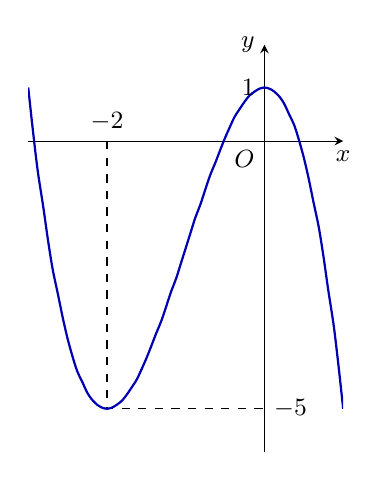
\begin{tikzpicture}[x=1cm,y=0.68cm,>=stealth,font=\small]
\draw[->] (-3,0)--(1,0) node[below]{$x$};
\draw[->] (0,-5.8)--(0,1.8) node[left]{$y$};
\node[below left] at (0,0){$O$};
\draw[dashed,thin] (-2,0)--(-2,-5)--(0,-5);
\begin{scope}\clip (-3,-5.81) rectangle (1,1.8);
\draw[thick,blue!70!black] plot[smooth] coordinates {(-3,1) (-2.94,0.19) (-2.88,-0.55) (-2.81,-1.22) (-2.75,-1.84) (-2.69,-2.39) (-2.62,-2.88) (-2.56,-3.31) (-2.5,-3.69) (-2.44,-4.01) (-2.38,-4.29) (-2.31,-4.51) (-2.25,-4.7) (-2.19,-4.83) (-2.12,-4.93) (-2.06,-4.98) (-2,-5) (-1.94,-4.98) (-1.88,-4.93) (-1.81,-4.85) (-1.75,-4.74) (-1.69,-4.61) (-1.62,-4.45) (-1.56,-4.26) (-1.5,-4.06) (-1.44,-3.84) (-1.38,-3.61) (-1.31,-3.36) (-1.25,-3.1) (-1.19,-2.83) (-1.12,-2.56) (-1.06,-2.28) (-1,-2) (-0.94,-1.72) (-0.88,-1.44) (-0.81,-1.17) (-0.75,-0.9) (-0.69,-0.64) (-0.62,-0.39) (-0.56,-0.16) (-0.5,0.06) (-0.44,0.26) (-0.38,0.45) (-0.31,0.61) (-0.25,0.74) (-0.19,0.85) (-0.12,0.93) (-0.06,0.98) (0,1) (0.06,0.98) (0.12,0.93) (0.19,0.83) (0.25,0.7) (0.31,0.51) (0.38,0.29) (0.44,0.01) (0.5,-0.31) (0.56,-0.69) (0.62,-1.12) (0.69,-1.61) (0.75,-2.16) (0.81,-2.78) (0.88,-3.45) (0.94,-4.19) (1,-5)};
\end{scope}
\node[above] at (-2,0){$-2$};
\node[right] at (0,-5){$-5$};
\node[left] at (0,1){$1$};
\end{tikzpicture}
\end{center}
Số nghiệm thực của phương trình $-2f(x)+4=0$ là}
  {$1$.}
  {$2$.}{$0$.}{$3$.}

\cauTN[id=C1-B4-D04-NB-021,muc=NB,loigiai={Phương trình hoành độ giao điểm: $x^{3}-3x-3=-1\Leftrightarrow x^{3}-3x-2=0\Leftrightarrow x=-1 \vee x=2$. Các giao điểm: $(-1;-1)$, $(2;-1)$.}]{Cho hàm số $y=x^{3}-3x-3$ có đồ thị $(C)$ và đường thẳng $d: y=-1$. Số giao điểm của $(C)$ và $d$ là}
  {$2$.}
  {$3$.}{$1$.}{$0$.}

\cauTN[id=C1-B4-D04-NB-022,muc=NB,loigiai={Phương trình hoành độ giao điểm: $-x^{3}+2x+1=x+1\Leftrightarrow -x^{3}+x=0\Leftrightarrow x=-1 \vee x=0 \vee x=1$. Các giao điểm: $(-1;0)$, $(0;1)$, $(1;2)$.}]{Cho hàm số $y=-x^{3}+2x+1$ có đồ thị $(C)$ và đường thẳng $d: y=x+1$. Tổng hoành độ các giao điểm của $(C)$ và $d$ bằng}
  {$0$.}
  {$1$.}{$-2$.}{$2$.}

\cauTN[id=C1-B4-D04-NB-023,muc=NB,loigiai={Số nghiệm của phương trình $f(x)=1$ bằng số giao điểm của đồ thị $y=f(x)$ với đường thẳng $y=1$. Dựa vào đồ thị ta được $2$ nghiệm.}]{Cho hàm số $y=f(x)$ có đồ thị như hình vẽ.
\begin{center}
\begin{tikzpicture}[x=1cm,y=1cm,>=stealth,font=\small]
\draw[->] (-3,0)--(3,0) node[below]{$x$};
\draw[->] (0,-0.8)--(0,3.8) node[left]{$y$};
\node[below left] at (0,0){$O$};
\draw[dashed,thin] (-2,0)--(-2,1)--(0,1);
\draw[dashed,thin] (2,0)--(2,3)--(0,3);
\begin{scope}\clip (-3,-0.81) rectangle (3,3.8);
\draw[thick,blue!70!black] plot[smooth] coordinates {(-3,1.44) (-2.91,1.35) (-2.81,1.28) (-2.72,1.22) (-2.62,1.16) (-2.53,1.12) (-2.44,1.08) (-2.34,1.05) (-2.25,1.02) (-2.16,1.01) (-2.06,1) (-1.97,1) (-1.88,1.01) (-1.78,1.02) (-1.69,1.03) (-1.59,1.06) (-1.5,1.09) (-1.41,1.12) (-1.31,1.16) (-1.22,1.2) (-1.12,1.25) (-1.03,1.3) (-0.94,1.35) (-0.84,1.4) (-0.75,1.46) (-0.66,1.53) (-0.56,1.59) (-0.47,1.65) (-0.38,1.72) (-0.28,1.79) (-0.19,1.86) (-0.09,1.93) (0,2) (0.09,2.07) (0.19,2.14) (0.28,2.21) (0.38,2.28) (0.47,2.35) (0.56,2.41) (0.66,2.47) (0.75,2.54) (0.84,2.6) (0.94,2.65) (1.03,2.7) (1.12,2.75) (1.22,2.8) (1.31,2.84) (1.41,2.88) (1.5,2.91) (1.59,2.94) (1.69,2.97) (1.78,2.98) (1.88,2.99) (1.97,3) (2.06,3) (2.16,2.99) (2.25,2.98) (2.34,2.95) (2.44,2.92) (2.53,2.88) (2.62,2.84) (2.72,2.78) (2.81,2.72) (2.91,2.65) (3,2.56)};
\end{scope}
\node[below] at (-2,0){$-2$};
\node[below] at (2,0){$2$};
\node[right] at (0,1){$1$};
\node[left] at (0,3){$3$};
\end{tikzpicture}
\end{center}
Số nghiệm thực của phương trình $f(x)=1$ là}
  {$2$.}
  {$3$.}{$1$.}{$4$.}

\cauTN[id=C1-B4-D04-NB-024,muc=NB,loigiai={Ta có $-2f(x)-10=0\Leftrightarrow f(x)=-5$. Số nghiệm bằng số giao điểm của đồ thị $y=f(x)$ với đường thẳng $y=-5$. Dựa vào bảng biến thiên ta được $2$ nghiệm.}]{Cho hàm số $y=f(x)$ xác định trên $\mathbb{R}\setminus\{-2\}$ và có bảng biến thiên như sau:
\begin{center}

\begin{tikzpicture}
\tkzTabInit[lgt=1.2,espcl=1.9]{$x$/0.7,$y'$/0.7,$y$/2}{$-\infty$,$-4$,$-2$,$0$,$+\infty$}
\tkzTabLine{ ,-,z,+,d,+,z,-, }
\tkzTabVar{+/$+\infty$,-/$5$,+D-/$+\infty$/$-\infty$,+/$-3$,-/$-\infty$}
\end{tikzpicture}
\end{center}
Số nghiệm thực của phương trình $-2f(x)-10=0$ là}
  {$2$.}
  {$3$.}{$1$.}{$4$.}

\cauTN[id=C1-B4-D04-NB-025,muc=NB,loigiai={Số nghiệm của phương trình $f(x)=1$ bằng số giao điểm của đồ thị $y=f(x)$ với đường thẳng $y=1$. Dựa vào bảng biến thiên ta được $0$ nghiệm.}]{Cho hàm số $y=f(x)$ xác định trên $\mathbb{R}\setminus\{-1\}$ và có bảng biến thiên như sau:
\begin{center}

\begin{tikzpicture}
\tkzTabInit[lgt=1.2,espcl=1.9]{$x$/0.7,$y'$/0.7,$y$/2}{$-\infty$,$-2$,$-1$,$0$,$+\infty$}
\tkzTabLine{ ,-,z,+,d,+,z,-, }
\tkzTabVar{+/$+\infty$,-/$2$,+D-/$+\infty$/$-\infty$,+/$-2$,-/$-\infty$}
\end{tikzpicture}
\end{center}
Số nghiệm thực của phương trình $f(x)=1$ là}
  {$0$.}
  {$1$.}{$2$.}{$3$.}

\cauTN[id=C1-B4-D04-NB-026,muc=NB,loigiai={Phương trình hoành độ giao điểm: $x^{3}+3x^{2}+x-1=x+3\Leftrightarrow x^{3}+3x^{2}-4=0\Leftrightarrow x=-2 \vee x=1$. Các giao điểm: $(-2;1)$, $(1;4)$.}]{Cho hàm số $y=x^{3}+3x^{2}+x-1$ có đồ thị $(C)$ và đường thẳng $d: y=x+3$. Điểm nào dưới đây là một giao điểm của $(C)$ và $d$?}
  {$(1;4)$.}
  {$(4;1)$.}{$(1;5)$.}{$(-1;4)$.}

\cauTN[id=C1-B4-D04-NB-027,muc=NB,loigiai={Số nghiệm của phương trình $f(x)=6$ bằng số giao điểm của đồ thị $y=f(x)$ với đường thẳng $y=6$. Dựa vào bảng biến thiên ta được $2$ nghiệm.}]{Cho hàm số $y=f(x)$ xác định trên $\mathbb{R}\setminus\{1\}$ và có bảng biến thiên như sau:
\begin{center}

\begin{tikzpicture}
\tkzTabInit[lgt=1.2,espcl=1.9]{$x$/0.7,$y'$/0.7,$y$/2}{$-\infty$,$0$,$1$,$2$,$+\infty$}
\tkzTabLine{ ,-,z,+,d,+,z,-, }
\tkzTabVar{+/$+\infty$,-/$4$,+D-/$+\infty$/$-\infty$,+/$0$,-/$-\infty$}
\end{tikzpicture}
\end{center}
Số nghiệm thực của phương trình $f(x)=6$ là}
  {$2$.}
  {$3$.}{$1$.}{$4$.}

\cauTN[id=C1-B4-D04-NB-028,muc=NB,loigiai={Ta có $-2f(x)+8=0\Leftrightarrow f(x)=4$. Số nghiệm bằng số giao điểm của đồ thị $y=f(x)$ với đường thẳng $y=4$. Dựa vào bảng biến thiên ta được $2$ nghiệm.}]{Cho hàm số $y=f(x)$ có bảng biến thiên như sau:
\begin{center}

\begin{tikzpicture}
\tkzTabInit[lgt=1.2,espcl=1.9]{$x$/0.7,$y'$/0.7,$y$/2}{$-\infty$,$1$,$3$,$+\infty$}
\tkzTabLine{ ,+,z,-,z,+, }
\tkzTabVar{-/$-\infty$,+/$4$,-/$-2$,+/$+\infty$}
\end{tikzpicture}
\end{center}
Số nghiệm thực của phương trình $-2f(x)+8=0$ là}
  {$2$.}
  {$3$.}{$1$.}{$4$.}

\cauTN[id=C1-B4-D04-NB-029,muc=NB,loigiai={Số nghiệm của phương trình $f(x)=7$ bằng số giao điểm của đồ thị $y=f(x)$ với đường thẳng $y=7$. Dựa vào bảng biến thiên ta được $2$ nghiệm.}]{Cho hàm số $y=f(x)$ xác định trên $\mathbb{R}\setminus\{-2\}$ và có bảng biến thiên như sau:
\begin{center}

\begin{tikzpicture}
\tkzTabInit[lgt=1.2,espcl=1.9]{$x$/0.7,$y'$/0.7,$y$/2}{$-\infty$,$-3$,$-2$,$-1$,$+\infty$}
\tkzTabLine{ ,-,z,+,d,+,z,-, }
\tkzTabVar{+/$+\infty$,-/$6$,+D-/$+\infty$/$-\infty$,+/$2$,-/$-\infty$}
\end{tikzpicture}
\end{center}
Số nghiệm thực của phương trình $f(x)=7$ là}
  {$2$.}
  {$3$.}{$1$.}{$4$.}

\cauTN[id=C1-B4-D04-NB-030,muc=NB,loigiai={Số nghiệm của phương trình $f(x)=6$ bằng số giao điểm của đồ thị $y=f(x)$ với đường thẳng $y=6$. Dựa vào bảng biến thiên ta được $1$ nghiệm.}]{Cho hàm số $y=f(x)$ có bảng biến thiên như sau:
\begin{center}

\begin{tikzpicture}
\tkzTabInit[lgt=1.2,espcl=1.9]{$x$/0.7,$y'$/0.7,$y$/2}{$-\infty$,$-3$,$-1$,$+\infty$}
\tkzTabLine{ ,+,z,-,z,+, }
\tkzTabVar{-/$-\infty$,+/$5$,-/$-3$,+/$+\infty$}
\end{tikzpicture}
\end{center}
Số nghiệm thực của phương trình $f(x)=6$ là}
  {$1$.}
  {$2$.}{$0$.}{$3$.}

\cauTN[id=C1-B4-D04-NB-031,muc=NB,loigiai={Phương trình hoành độ giao điểm: $x^{3}-2x^{2}-3x+5=-2x+3\Leftrightarrow x^{3}-2x^{2}-x+2=0\Leftrightarrow x=-1 \vee x=1 \vee x=2$. Các giao điểm: $(-1;5)$, $(1;1)$, $(2;-1)$.}]{Cho hàm số $y=x^{3}-2x^{2}-3x+5$ có đồ thị $(C)$ và đường thẳng $d: y=-2x+3$. Điểm nào dưới đây là một giao điểm của $(C)$ và $d$?}
  {$(-1;5)$.}
  {$(5;-1)$.}{$(-1;6)$.}{$(1;5)$.}

\cauTN[id=C1-B4-D04-NB-032,muc=NB,loigiai={Phương trình hoành độ giao điểm: $-x^{3}+5x^{2}-5x+2=2x-1\Leftrightarrow -x^{3}+5x^{2}-7x+3=0\Leftrightarrow x=1 \vee x=3$. Các giao điểm: $(1;1)$, $(3;5)$.}]{Cho hàm số $y=-x^{3}+5x^{2}-5x+2$ có đồ thị $(C)$ và đường thẳng $d: y=2x-1$. Tổng hoành độ các giao điểm của $(C)$ và $d$ bằng}
  {$4$.}
  {$3$.}{$5$.}{$2$.}

\cauTN[id=C1-B4-D04-NB-033,muc=NB,loigiai={Phương trình hoành độ giao điểm: $x^{3}+x^{2}-2x-2=2x+2\Leftrightarrow x^{3}+x^{2}-4x-4=0\Leftrightarrow x=-2 \vee x=-1 \vee x=2$. Các giao điểm: $(-2;-2)$, $(-1;0)$, $(2;6)$.}]{Cho hàm số $y=x^{3}+x^{2}-2x-2$ có đồ thị $(C)$ và đường thẳng $d: y=2x+2$. Điểm nào dưới đây là một giao điểm của $(C)$ và $d$?}
  {$(-1;0)$.}
  {$(0;-1)$.}{$(-1;1)$.}{$(1;0)$.}

\cauTN[id=C1-B4-D04-NB-034,muc=NB,loigiai={Số nghiệm của phương trình $f(x)=1$ bằng số giao điểm của đồ thị $y=f(x)$ với đường thẳng $y=1$. Dựa vào bảng biến thiên ta được $0$ nghiệm.}]{Cho hàm số $y=f(x)$ xác định trên $\mathbb{R}\setminus\{-2\}$ và có bảng biến thiên như sau:
\begin{center}

\begin{tikzpicture}
\tkzTabInit[lgt=1.2,espcl=1.9]{$x$/0.7,$y'$/0.7,$y$/2}{$-\infty$,$-3$,$-2$,$-1$,$+\infty$}
\tkzTabLine{ ,+,z,-,d,-,z,+, }
\tkzTabVar{-/$-\infty$,+/$-2$,-D+/$-\infty$/$+\infty$,-/$2$,+/$+\infty$}
\end{tikzpicture}
\end{center}
Số nghiệm thực của phương trình $f(x)=1$ là}
  {$0$.}
  {$1$.}{$2$.}{$3$.}

\cauTN[id=C1-B4-D04-NB-035,muc=NB,loigiai={Phương trình hoành độ giao điểm: $x^{3}+6x^{2}+11x+2=2x+2\Leftrightarrow x^{3}+6x^{2}+9x=0\Leftrightarrow x=-3 \vee x=0$. Các giao điểm: $(-3;-4)$, $(0;2)$.}]{Cho hàm số $y=x^{3}+6x^{2}+11x+2$ có đồ thị $(C)$ và đường thẳng $d: y=2x+2$. Tổng hoành độ các giao điểm của $(C)$ và $d$ bằng}
  {$-3$.}
  {$0$.}{$3$.}{$-1$.}

\cauTN[id=C1-B4-D04-NB-036,muc=NB,loigiai={Phương trình hoành độ giao điểm: $-x^{3}-x^{2}+x=x\Leftrightarrow -x^{3}-x^{2}=0\Leftrightarrow x=-1 \vee x=0$. Các giao điểm: $(-1;-1)$, $(0;0)$.}]{Cho hàm số $y=-x^{3}-x^{2}+x$ có đồ thị $(C)$ và đường thẳng $d: y=x$. Tổng hoành độ các giao điểm của $(C)$ và $d$ bằng}
  {$-1$.}
  {$0$.}{$1$.}{$-3$.}

\cauDS[id=C1-B4-D04-NB-037,muc=NB,loigiai={Dựa vào bảng biến thiên, xét số giao điểm của đồ thị $y=f(x)$ với các đường thẳng nằm ngang tương ứng. a) Đúng. b) Đúng. c) Đúng. d) Sai: phương trình có $2$ nghiệm.}]{Cho hàm số $y=f(x)$ xác định trên $\mathbb{R}\setminus\{1\}$ và có bảng biến thiên như sau:
\begin{center}

\begin{tikzpicture}
\tkzTabInit[lgt=1.2,espcl=1.9]{$x$/0.7,$y'$/0.7,$y$/2}{$-\infty$,$0$,$1$,$2$,$+\infty$}
\tkzTabLine{ ,+,z,-,d,-,z,+, }
\tkzTabVar{-/$-\infty$,+/$-4$,-D+/$-\infty$/$+\infty$,-/$0$,+/$+\infty$}
\end{tikzpicture}
\end{center}
Xét tính đúng sai của các mệnh đề sau:}{%
  \y{Phương trình $f(x)=-4$ có đúng $1$ nghiệm thực.}{d}
  \y{Phương trình $f(x)=-1$ có đúng $0$ nghiệm thực.}{d}
  \y{Phương trình $f(x)=2$ có đúng $2$ nghiệm thực.}{d}
  \y{Phương trình $f(x)=1$ có đúng $3$ nghiệm thực.}{s}}

\cauDS[id=C1-B4-D04-NB-038,muc=NB,loigiai={Dựa vào đồ thị, xét số giao điểm của đồ thị $y=f(x)$ với các đường thẳng nằm ngang tương ứng. a) Đúng. b) Sai: phương trình có $1$ nghiệm. c) Đúng. d) Sai: phương trình có $3$ nghiệm.}]{Cho hàm số $y=f(x)$ có đồ thị như hình vẽ.
\begin{center}
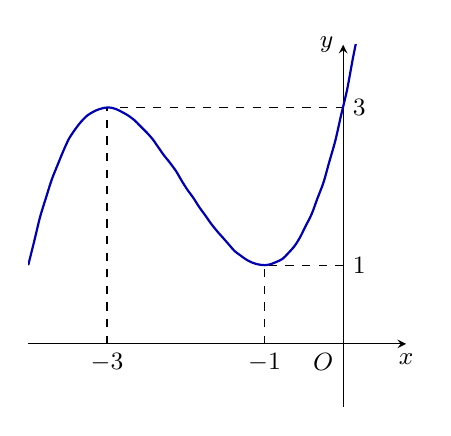
\begin{tikzpicture}[x=1cm,y=1cm,>=stealth,font=\small]
\draw[->] (-4,0)--(0.8,0) node[below]{$x$};
\draw[->] (0,-0.8)--(0,3.8) node[left]{$y$};
\node[below left] at (0,0){$O$};
\draw[dashed,thin] (-3,0)--(-3,3)--(0,3);
\draw[dashed,thin] (-1,0)--(-1,1)--(0,1);
\begin{scope}\clip (-4,-0.81) rectangle (0.8,3.8);
\draw[thick,blue!70!black] plot[smooth] coordinates {(-4,1) (-3.92,1.32) (-3.85,1.61) (-3.77,1.87) (-3.7,2.09) (-3.62,2.29) (-3.55,2.46) (-3.48,2.61) (-3.4,2.73) (-3.33,2.82) (-3.25,2.9) (-3.17,2.95) (-3.1,2.98) (-3.02,3) (-2.95,3) (-2.88,2.98) (-2.8,2.94) (-2.73,2.9) (-2.65,2.84) (-2.58,2.77) (-2.5,2.69) (-2.42,2.6) (-2.35,2.5) (-2.28,2.4) (-2.2,2.3) (-2.12,2.19) (-2.05,2.07) (-1.98,1.96) (-1.9,1.85) (-1.83,1.74) (-1.75,1.63) (-1.68,1.53) (-1.6,1.43) (-1.52,1.34) (-1.45,1.26) (-1.38,1.18) (-1.3,1.12) (-1.23,1.07) (-1.15,1.03) (-1.08,1.01) (-1,1) (-0.93,1.01) (-0.85,1.04) (-0.77,1.08) (-0.7,1.15) (-0.62,1.24) (-0.55,1.35) (-0.48,1.49) (-0.4,1.65) (-0.33,1.84) (-0.25,2.05) (-0.18,2.3) (-0.1,2.58) (-0.03,2.89) (0.05,3.23) (0.12,3.61) (0.2,4.02) (0.27,4.47) (0.35,4.96) (0.42,5.49) (0.5,6.06) (0.58,6.67) (0.65,6.8) (0.72,6.8) (0.8,6.8)};
\end{scope}
\node[below] at (-3,0){$-3$};
\node[below] at (-1,0){$-1$};
\node[right] at (0,1){$1$};
\node[right] at (0,3){$3$};
\end{tikzpicture}
\end{center}
Xét tính đúng sai của các mệnh đề sau:}{%
  \y{Phương trình $f(x)=0$ có đúng $1$ nghiệm thực.}{d}
  \y{Phương trình $-2f(x)-2=0$ có đúng $0$ nghiệm thực.}{s}
  \y{Phương trình $3f(x)-15=0$ có đúng $1$ nghiệm thực.}{d}
  \y{Phương trình $-2f(x)+4=0$ có đúng $2$ nghiệm thực.}{s}}

\cauDS[id=C1-B4-D04-NB-039,muc=NB,loigiai={Dựa vào đồ thị, xét số giao điểm của đồ thị $y=f(x)$ với các đường thẳng nằm ngang tương ứng. a) Sai: phương trình có $1$ nghiệm. b) Sai: phương trình có $1$ nghiệm. c) Đúng. d) Sai: phương trình có $1$ nghiệm.}]{Cho hàm số $y=f(x)$ có đồ thị như hình vẽ.
\begin{center}
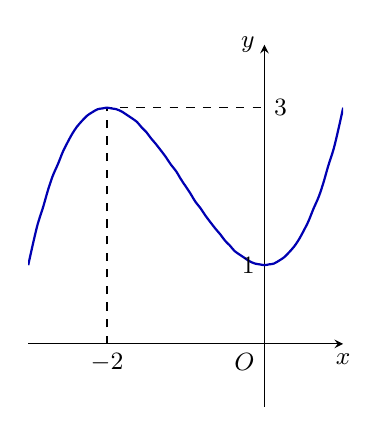
\begin{tikzpicture}[x=1cm,y=1cm,>=stealth,font=\small]
\draw[->] (-3,0)--(1,0) node[below]{$x$};
\draw[->] (0,-0.8)--(0,3.8) node[left]{$y$};
\node[below left] at (0,0){$O$};
\draw[dashed,thin] (-2,0)--(-2,3)--(0,3);
\begin{scope}\clip (-3,-0.81) rectangle (1,3.8);
\draw[thick,blue!70!black] plot[smooth] coordinates {(-3,1) (-2.94,1.27) (-2.88,1.52) (-2.81,1.74) (-2.75,1.95) (-2.69,2.13) (-2.62,2.29) (-2.56,2.44) (-2.5,2.56) (-2.44,2.67) (-2.38,2.76) (-2.31,2.84) (-2.25,2.9) (-2.19,2.94) (-2.12,2.98) (-2.06,2.99) (-2,3) (-1.94,2.99) (-1.88,2.98) (-1.81,2.95) (-1.75,2.91) (-1.69,2.87) (-1.62,2.82) (-1.56,2.75) (-1.5,2.69) (-1.44,2.61) (-1.38,2.54) (-1.31,2.45) (-1.25,2.37) (-1.19,2.28) (-1.12,2.19) (-1.06,2.09) (-1,2) (-0.94,1.91) (-0.88,1.81) (-0.81,1.72) (-0.75,1.63) (-0.69,1.55) (-0.62,1.46) (-0.56,1.39) (-0.5,1.31) (-0.44,1.25) (-0.38,1.18) (-0.31,1.13) (-0.25,1.09) (-0.19,1.05) (-0.12,1.02) (-0.06,1.01) (0,1) (0.06,1.01) (0.12,1.02) (0.19,1.06) (0.25,1.1) (0.31,1.16) (0.38,1.24) (0.44,1.33) (0.5,1.44) (0.56,1.56) (0.62,1.71) (0.69,1.87) (0.75,2.05) (0.81,2.26) (0.88,2.48) (0.94,2.73) (1,3)};
\end{scope}
\node[below] at (-2,0){$-2$};
\node[left] at (0,1){$1$};
\node[right] at (0,3){$3$};
\end{tikzpicture}
\end{center}
Xét tính đúng sai của các mệnh đề sau:}{%
  \y{Phương trình $f(x)=4$ có đúng $2$ nghiệm thực.}{s}
  \y{Phương trình $3f(x)-15=0$ có đúng $3$ nghiệm thực.}{s}
  \y{Phương trình $-2f(x)+4=0$ có đúng $3$ nghiệm thực.}{d}
  \y{Phương trình $f(x)=0$ có đúng $2$ nghiệm thực.}{s}}

\cauDS[id=C1-B4-D04-NB-040,muc=NB,loigiai={Dựa vào bảng biến thiên, xét số giao điểm của đồ thị $y=f(x)$ với các đường thẳng nằm ngang tương ứng. a) Đúng. b) Đúng. c) Sai: phương trình có $1$ nghiệm. d) Sai: phương trình có $1$ nghiệm.}]{Cho hàm số $y=f(x)$ có bảng biến thiên như sau:
\begin{center}

\begin{tikzpicture}
\tkzTabInit[lgt=1.2,espcl=1.9]{$x$/0.7,$y'$/0.7,$y$/2}{$-\infty$,$-1$,$1$,$+\infty$}
\tkzTabLine{ ,+,z,-,z,+, }
\tkzTabVar{-/$-\infty$,+/$1$,-/$-3$,+/$+\infty$}
\end{tikzpicture}
\end{center}
Xét tính đúng sai của các mệnh đề sau:}{%
  \y{Phương trình $f(x)=-5$ có đúng $1$ nghiệm thực.}{d}
  \y{Phương trình $f(x)=-4$ có đúng $1$ nghiệm thực.}{d}
  \y{Phương trình $-2f(x)-10=0$ có đúng $3$ nghiệm thực.}{s}
  \y{Phương trình $3f(x)+12=0$ có đúng $0$ nghiệm thực.}{s}}

\cauDS[id=C1-B4-D04-NB-041,muc=NB,loigiai={Dựa vào bảng biến thiên, xét số giao điểm của đồ thị $y=f(x)$ với các đường thẳng nằm ngang tương ứng. a) Sai: phương trình có $1$ nghiệm. b) Đúng. c) Sai: phương trình có $1$ nghiệm. d) Sai: phương trình có $2$ nghiệm.}]{Cho hàm số $y=f(x)$ có bảng biến thiên như sau:
\begin{center}

\begin{tikzpicture}
\tkzTabInit[lgt=1.2,espcl=1.9]{$x$/0.7,$y'$/0.7,$y$/2}{$-\infty$,$-2$,$2$,$+\infty$}
\tkzTabLine{ ,+,z,-,z,+, }
\tkzTabVar{-/$-\infty$,+/$-3$,-/$-5$,+/$+\infty$}
\end{tikzpicture}
\end{center}
Xét tính đúng sai của các mệnh đề sau:}{%
  \y{Phương trình $-2f(x)-12=0$ có đúng $3$ nghiệm thực.}{s}
  \y{Phương trình $f(x)=-4$ có đúng $3$ nghiệm thực.}{d}
  \y{Phương trình $f(x)=-7$ có đúng $2$ nghiệm thực.}{s}
  \y{Phương trình $f(x)=-3$ có đúng $1$ nghiệm thực.}{s}}

\cauDS[id=C1-B4-D04-NB-042,muc=NB,loigiai={Dựa vào đồ thị, xét số giao điểm của đồ thị $y=f(x)$ với các đường thẳng nằm ngang tương ứng. a) Đúng. b) Sai: phương trình có $2$ nghiệm. c) Sai: phương trình có $1$ nghiệm. d) Đúng.}]{Cho hàm số $y=f(x)$ có đồ thị như hình vẽ.
\begin{center}
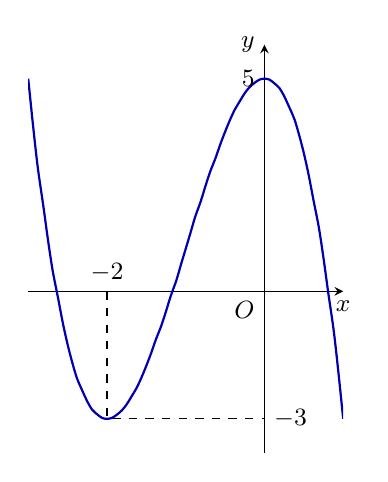
\begin{tikzpicture}[x=1cm,y=0.54cm,>=stealth,font=\small]
\draw[->] (-3,0)--(1,0) node[below]{$x$};
\draw[->] (0,-3.8)--(0,5.8) node[left]{$y$};
\node[below left] at (0,0){$O$};
\draw[dashed,thin] (-2,0)--(-2,-3)--(0,-3);
\begin{scope}\clip (-3,-3.81) rectangle (1,5.8);
\draw[thick,blue!70!black] plot[smooth] coordinates {(-3,5) (-2.94,3.92) (-2.88,2.93) (-2.81,2.03) (-2.75,1.22) (-2.69,0.49) (-2.62,-0.17) (-2.56,-0.75) (-2.5,-1.25) (-2.44,-1.68) (-2.38,-2.05) (-2.31,-2.35) (-2.25,-2.59) (-2.19,-2.78) (-2.12,-2.9) (-2.06,-2.98) (-2,-3) (-1.94,-2.98) (-1.88,-2.91) (-1.81,-2.8) (-1.75,-2.66) (-1.69,-2.48) (-1.62,-2.26) (-1.56,-2.02) (-1.5,-1.75) (-1.44,-1.46) (-1.38,-1.14) (-1.31,-0.81) (-1.25,-0.47) (-1.19,-0.11) (-1.12,0.25) (-1.06,0.63) (-1,1) (-0.94,1.37) (-0.88,1.75) (-0.81,2.11) (-0.75,2.47) (-0.69,2.81) (-0.62,3.14) (-0.56,3.46) (-0.5,3.75) (-0.44,4.02) (-0.38,4.26) (-0.31,4.48) (-0.25,4.66) (-0.19,4.8) (-0.12,4.91) (-0.06,4.98) (0,5) (0.06,4.98) (0.12,4.9) (0.19,4.78) (0.25,4.59) (0.31,4.35) (0.38,4.05) (0.44,3.68) (0.5,3.25) (0.56,2.75) (0.62,2.17) (0.69,1.51) (0.75,0.78) (0.81,-0.03) (0.88,-0.93) (0.94,-1.92) (1,-3)};
\end{scope}
\node[above] at (-2,0){$-2$};
\node[right] at (0,-3){$-3$};
\node[left] at (0,5){$5$};
\end{tikzpicture}
\end{center}
Xét tính đúng sai của các mệnh đề sau:}{%
  \y{Phương trình $f(x)=-4$ có đúng $1$ nghiệm thực.}{d}
  \y{Phương trình $f(x)=-3$ có đúng $1$ nghiệm thực.}{s}
  \y{Phương trình $f(x)=-5$ có đúng $2$ nghiệm thực.}{s}
  \y{Phương trình $-2f(x)+10=0$ có đúng $2$ nghiệm thực.}{d}}

\cauDS[id=C1-B4-D04-NB-043,muc=NB,loigiai={Dựa vào bảng biến thiên, xét số giao điểm của đồ thị $y=f(x)$ với các đường thẳng nằm ngang tương ứng. a) Đúng. b) Đúng. c) Sai: phương trình có $1$ nghiệm. d) Đúng.}]{Cho hàm số $y=f(x)$ có bảng biến thiên như sau:
\begin{center}

\begin{tikzpicture}
\tkzTabInit[lgt=1.2,espcl=1.9]{$x$/0.7,$y'$/0.7,$y$/2}{$-\infty$,$-2$,$0$,$+\infty$}
\tkzTabLine{ ,+,z,-,z,+, }
\tkzTabVar{-/$-\infty$,+/$-3$,-/$-5$,+/$+\infty$}
\end{tikzpicture}
\end{center}
Xét tính đúng sai của các mệnh đề sau:}{%
  \y{Phương trình $f(x)=-1$ có đúng $1$ nghiệm thực.}{d}
  \y{Phương trình $3f(x)+9=0$ có đúng $2$ nghiệm thực.}{d}
  \y{Phương trình $f(x)=-7$ có đúng $2$ nghiệm thực.}{s}
  \y{Phương trình $f(x)=-4$ có đúng $3$ nghiệm thực.}{d}}

\cauDS[id=C1-B4-D04-NB-044,muc=NB,loigiai={Dựa vào bảng biến thiên, xét số giao điểm của đồ thị $y=f(x)$ với các đường thẳng nằm ngang tương ứng. a) Đúng. b) Sai: phương trình có $2$ nghiệm. c) Đúng. d) Đúng.}]{Cho hàm số $y=f(x)$ có bảng biến thiên như sau:
\begin{center}

\begin{tikzpicture}
\tkzTabInit[lgt=1.2,espcl=1.9]{$x$/0.7,$y'$/0.7,$y$/2}{$-\infty$,$1$,$3$,$+\infty$}
\tkzTabLine{ ,+,z,-,z,+, }
\tkzTabVar{-/$-\infty$,+/$0$,-/$-2$,+/$+\infty$}
\end{tikzpicture}
\end{center}
Xét tính đúng sai của các mệnh đề sau:}{%
  \y{Phương trình $f(x)=-2$ có đúng $2$ nghiệm thực.}{d}
  \y{Phương trình $f(x)=0$ có đúng $3$ nghiệm thực.}{s}
  \y{Phương trình $f(x)=2$ có đúng $1$ nghiệm thực.}{d}
  \y{Phương trình $f(x)=-4$ có đúng $1$ nghiệm thực.}{d}}

\cauDS[id=C1-B4-D04-NB-045,muc=NB,loigiai={Dựa vào bảng biến thiên, xét số giao điểm của đồ thị $y=f(x)$ với các đường thẳng nằm ngang tương ứng. a) Sai: phương trình có $2$ nghiệm. b) Sai: phương trình có $1$ nghiệm. c) Sai: phương trình có $2$ nghiệm. d) Đúng.}]{Cho hàm số $y=f(x)$ xác định trên $\mathbb{R}\setminus\{0\}$ và có bảng biến thiên như sau:
\begin{center}

\begin{tikzpicture}
\tkzTabInit[lgt=1.2,espcl=1.9]{$x$/0.7,$y'$/0.7,$y$/2}{$-\infty$,$-2$,$0$,$2$,$+\infty$}
\tkzTabLine{ ,+,z,-,d,-,z,+, }
\tkzTabVar{-/$-\infty$,+/$-3$,-D+/$-\infty$/$+\infty$,-/$5$,+/$+\infty$}
\end{tikzpicture}
\end{center}
Xét tính đúng sai của các mệnh đề sau:}{%
  \y{Phương trình $-2f(x)+14=0$ có đúng $1$ nghiệm thực.}{s}
  \y{Phương trình $-2f(x)-6=0$ có đúng $2$ nghiệm thực.}{s}
  \y{Phương trình $f(x)=-5$ có đúng $3$ nghiệm thực.}{s}
  \y{Phương trình $3f(x)-21=0$ có đúng $2$ nghiệm thực.}{d}}

\cauDS[id=C1-B4-D04-NB-046,muc=NB,loigiai={Dựa vào đồ thị, xét số giao điểm của đồ thị $y=f(x)$ với các đường thẳng nằm ngang tương ứng. a) Đúng. b) Sai: phương trình có $1$ nghiệm. c) Đúng. d) Đúng.}]{Cho hàm số $y=f(x)$ có đồ thị như hình vẽ.
\begin{center}
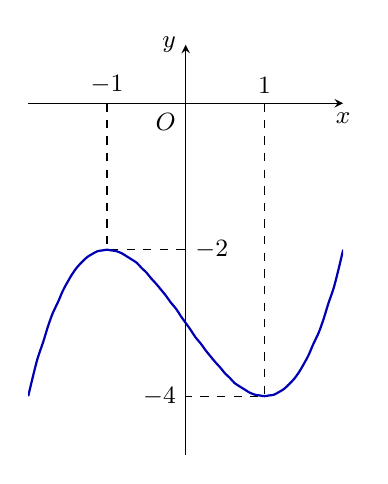
\begin{tikzpicture}[x=1cm,y=0.93cm,>=stealth,font=\small]
\draw[->] (-2,0)--(2,0) node[below]{$x$};
\draw[->] (0,-4.8)--(0,0.8) node[left]{$y$};
\node[below left] at (0,0){$O$};
\draw[dashed,thin] (-1,0)--(-1,-2)--(0,-2);
\draw[dashed,thin] (1,0)--(1,-4)--(0,-4);
\begin{scope}\clip (-2,-4.81) rectangle (2,0.8);
\draw[thick,blue!70!black] plot[smooth] coordinates {(-2,-4) (-1.94,-3.73) (-1.88,-3.48) (-1.81,-3.26) (-1.75,-3.05) (-1.69,-2.87) (-1.62,-2.71) (-1.56,-2.56) (-1.5,-2.44) (-1.44,-2.33) (-1.38,-2.24) (-1.31,-2.16) (-1.25,-2.1) (-1.19,-2.06) (-1.12,-2.02) (-1.06,-2.01) (-1,-2) (-0.94,-2.01) (-0.88,-2.02) (-0.81,-2.05) (-0.75,-2.09) (-0.69,-2.13) (-0.62,-2.18) (-0.56,-2.25) (-0.5,-2.31) (-0.44,-2.39) (-0.38,-2.46) (-0.31,-2.55) (-0.25,-2.63) (-0.19,-2.72) (-0.12,-2.81) (-0.06,-2.91) (0,-3) (0.06,-3.09) (0.12,-3.19) (0.19,-3.28) (0.25,-3.37) (0.31,-3.45) (0.38,-3.54) (0.44,-3.61) (0.5,-3.69) (0.56,-3.75) (0.62,-3.82) (0.69,-3.87) (0.75,-3.91) (0.81,-3.95) (0.88,-3.98) (0.94,-3.99) (1,-4) (1.06,-3.99) (1.12,-3.98) (1.19,-3.94) (1.25,-3.9) (1.31,-3.84) (1.38,-3.76) (1.44,-3.67) (1.5,-3.56) (1.56,-3.44) (1.62,-3.29) (1.69,-3.13) (1.75,-2.95) (1.81,-2.74) (1.88,-2.52) (1.94,-2.27) (2,-2)};
\end{scope}
\node[above] at (-1,0){$-1$};
\node[above] at (1,0){$1$};
\node[left] at (0,-4){$-4$};
\node[right] at (0,-2){$-2$};
\end{tikzpicture}
\end{center}
Xét tính đúng sai của các mệnh đề sau:}{%
  \y{Phương trình $f(x)=-6$ có đúng $1$ nghiệm thực.}{d}
  \y{Phương trình $f(x)=-1$ có đúng $2$ nghiệm thực.}{s}
  \y{Phương trình $2f(x)+6=0$ có đúng $3$ nghiệm thực.}{d}
  \y{Phương trình $f(x)=0$ có đúng $1$ nghiệm thực.}{d}}

\cauDS[id=C1-B4-D04-NB-047,muc=NB,loigiai={Dựa vào bảng biến thiên, xét số giao điểm của đồ thị $y=f(x)$ với các đường thẳng nằm ngang tương ứng. a) Đúng. b) Đúng. c) Sai: phương trình có $2$ nghiệm. d) Đúng.}]{Cho hàm số $y=f(x)$ xác định trên $\mathbb{R}\setminus\{-2\}$ và có bảng biến thiên như sau:
\begin{center}

\begin{tikzpicture}
\tkzTabInit[lgt=1.2,espcl=1.9]{$x$/0.7,$y'$/0.7,$y$/2}{$-\infty$,$-3$,$-2$,$-1$,$+\infty$}
\tkzTabLine{ ,-,z,+,d,+,z,-, }
\tkzTabVar{+/$+\infty$,-/$6$,+D-/$+\infty$/$-\infty$,+/$2$,-/$-\infty$}
\end{tikzpicture}
\end{center}
Xét tính đúng sai của các mệnh đề sau:}{%
  \y{Phương trình $f(x)=3$ có đúng $0$ nghiệm thực.}{d}
  \y{Phương trình $f(x)=5$ có đúng $0$ nghiệm thực.}{d}
  \y{Phương trình $3f(x)-3=0$ có đúng $4$ nghiệm thực.}{s}
  \y{Phương trình $f(x)=6$ có đúng $1$ nghiệm thực.}{d}}

\cauDS[id=C1-B4-D04-NB-048,muc=NB,loigiai={Dựa vào đồ thị, xét số giao điểm của đồ thị $y=f(x)$ với các đường thẳng nằm ngang tương ứng. a) Sai: phương trình có $1$ nghiệm. b) Đúng. c) Đúng. d) Sai: phương trình có $1$ nghiệm.}]{Cho hàm số $y=f(x)$ có đồ thị như hình vẽ.
\begin{center}
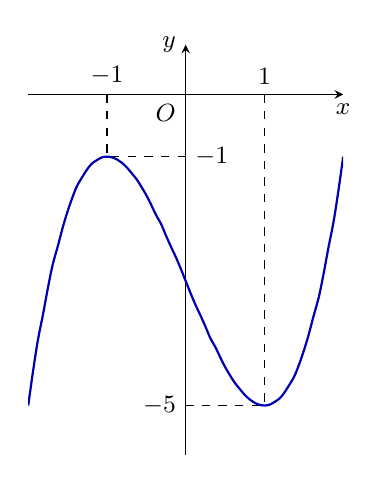
\begin{tikzpicture}[x=1cm,y=0.79cm,>=stealth,font=\small]
\draw[->] (-2,0)--(2,0) node[below]{$x$};
\draw[->] (0,-5.8)--(0,0.8) node[left]{$y$};
\node[below left] at (0,0){$O$};
\draw[dashed,thin] (-1,0)--(-1,-1)--(0,-1);
\draw[dashed,thin] (1,0)--(1,-5)--(0,-5);
\begin{scope}\clip (-2,-5.81) rectangle (2,0.8);
\draw[thick,blue!70!black] plot[smooth] coordinates {(-2,-5) (-1.94,-4.46) (-1.88,-3.97) (-1.81,-3.52) (-1.75,-3.11) (-1.69,-2.74) (-1.62,-2.42) (-1.56,-2.13) (-1.5,-1.88) (-1.44,-1.66) (-1.38,-1.47) (-1.31,-1.32) (-1.25,-1.2) (-1.19,-1.11) (-1.12,-1.05) (-1.06,-1.01) (-1,-1) (-0.94,-1.01) (-0.88,-1.04) (-0.81,-1.1) (-0.75,-1.17) (-0.69,-1.26) (-0.62,-1.37) (-0.56,-1.49) (-0.5,-1.62) (-0.44,-1.77) (-0.38,-1.93) (-0.31,-2.09) (-0.25,-2.27) (-0.19,-2.44) (-0.12,-2.63) (-0.06,-2.81) (0,-3) (0.06,-3.19) (0.12,-3.37) (0.19,-3.56) (0.25,-3.73) (0.31,-3.91) (0.38,-4.07) (0.44,-4.23) (0.5,-4.38) (0.56,-4.51) (0.62,-4.63) (0.69,-4.74) (0.75,-4.83) (0.81,-4.9) (0.88,-4.96) (0.94,-4.99) (1,-5) (1.06,-4.99) (1.12,-4.95) (1.19,-4.89) (1.25,-4.8) (1.31,-4.68) (1.38,-4.53) (1.44,-4.34) (1.5,-4.12) (1.56,-3.87) (1.62,-3.58) (1.69,-3.26) (1.75,-2.89) (1.81,-2.48) (1.88,-2.03) (1.94,-1.54) (2,-1)};
\end{scope}
\node[above] at (-1,0){$-1$};
\node[above] at (1,0){$1$};
\node[left] at (0,-5){$-5$};
\node[right] at (0,-1){$-1$};
\end{tikzpicture}
\end{center}
Xét tính đúng sai của các mệnh đề sau:}{%
  \y{Phương trình $2f(x)=0$ có đúng $3$ nghiệm thực.}{s}
  \y{Phương trình $3f(x)=0$ có đúng $1$ nghiệm thực.}{d}
  \y{Phương trình $f(x)=1$ có đúng $1$ nghiệm thực.}{d}
  \y{Phương trình $f(x)=-6$ có đúng $0$ nghiệm thực.}{s}}

\cauTLN[id=C1-B4-D04-NB-049,muc=NB,loigiai={Số nghiệm của phương trình $f(x)=1$ bằng số giao điểm của đồ thị $y=f(x)$ với đường thẳng $y=1$. Vậy có $0$ nghiệm.}]{Cho hàm số $y=f(x)$ xác định trên $\mathbb{R}\setminus\{-2\}$ và có bảng biến thiên như sau:
\begin{center}

\begin{tikzpicture}
\tkzTabInit[lgt=1.2,espcl=1.9]{$x$/0.7,$y'$/0.7,$y$/2}{$-\infty$,$-3$,$-2$,$-1$,$+\infty$}
\tkzTabLine{ ,-,z,+,d,+,z,-, }
\tkzTabVar{+/$+\infty$,-/$4$,+D-/$+\infty$/$-\infty$,+/$0$,-/$-\infty$}
\end{tikzpicture}
\end{center}
Phương trình $f(x)=1$ có bao nhiêu nghiệm thực?}{0}

\cauTLN[id=C1-B4-D04-NB-050,muc=NB,loigiai={Số nghiệm của phương trình $f(x)=3$ bằng số giao điểm của đồ thị $y=f(x)$ với đường thẳng $y=3$. Vậy có $2$ nghiệm.}]{Cho hàm số $y=f(x)$ có bảng biến thiên như sau:
\begin{center}

\begin{tikzpicture}
\tkzTabInit[lgt=1.2,espcl=1.9]{$x$/0.7,$y'$/0.7,$y$/2}{$-\infty$,$-1$,$1$,$+\infty$}
\tkzTabLine{ ,+,z,-,z,+, }
\tkzTabVar{-/$-\infty$,+/$3$,-/$-1$,+/$+\infty$}
\end{tikzpicture}
\end{center}
Phương trình $f(x)=3$ có bao nhiêu nghiệm thực?}{2}

\cauTLN[id=C1-B4-D04-NB-051,muc=NB,loigiai={Ta có $2f(x)+6=0\Leftrightarrow f(x)=-3$. Số nghiệm bằng số giao điểm của đồ thị $y=f(x)$ với đường thẳng $y=-3$. Vậy có $2$ nghiệm.}]{Cho hàm số $y=f(x)$ có bảng biến thiên như sau:
\begin{center}

\begin{tikzpicture}
\tkzTabInit[lgt=1.2,espcl=1.9]{$x$/0.7,$y'$/0.7,$y$/2}{$-\infty$,$-1$,$1$,$+\infty$}
\tkzTabLine{ ,-,z,+,z,-, }
\tkzTabVar{+/$+\infty$,-/$-5$,+/$-3$,-/$-\infty$}
\end{tikzpicture}
\end{center}
Phương trình $2f(x)+6=0$ có bao nhiêu nghiệm thực?}{2}

\cauTLN[id=C1-B4-D04-NB-052,muc=NB,loigiai={Số nghiệm của phương trình $f(x)=-4$ bằng số giao điểm của đồ thị $y=f(x)$ với đường thẳng $y=-4$. Vậy có $1$ nghiệm.}]{Cho hàm số $y=f(x)$ có đồ thị như hình vẽ.
\begin{center}
\begin{tikzpicture}[x=1cm,y=0.68cm,>=stealth,font=\small]
\draw[->] (-4,0)--(1,0) node[below]{$x$};
\draw[->] (0,-2.8)--(0,4.8) node[left]{$y$};
\node[below left] at (0,0){$O$};
\draw[dashed,thin] (-3,0)--(-3,4)--(0,4);
\begin{scope}\clip (-4,-2.81) rectangle (1,4.8);
\draw[thick,blue!70!black] plot[smooth] coordinates {(-4,1.56) (-3.92,1.95) (-3.84,2.31) (-3.77,2.63) (-3.69,2.91) (-3.61,3.16) (-3.53,3.37) (-3.45,3.55) (-3.38,3.7) (-3.3,3.81) (-3.22,3.9) (-3.14,3.96) (-3.06,3.99) (-2.98,4) (-2.91,3.98) (-2.83,3.94) (-2.75,3.88) (-2.67,3.8) (-2.59,3.7) (-2.52,3.58) (-2.44,3.45) (-2.36,3.3) (-2.28,3.13) (-2.2,2.95) (-2.12,2.77) (-2.05,2.57) (-1.97,2.36) (-1.89,2.15) (-1.81,1.92) (-1.73,1.7) (-1.66,1.47) (-1.58,1.23) (-1.5,1) (-1.42,0.77) (-1.34,0.53) (-1.27,0.3) (-1.19,0.08) (-1.11,-0.15) (-1.03,-0.36) (-0.95,-0.57) (-0.88,-0.77) (-0.8,-0.95) (-0.72,-1.13) (-0.64,-1.3) (-0.56,-1.45) (-0.48,-1.58) (-0.41,-1.7) (-0.33,-1.8) (-0.25,-1.88) (-0.17,-1.94) (-0.09,-1.98) (-0.02,-2) (0.06,-1.99) (0.14,-1.96) (0.22,-1.9) (0.3,-1.81) (0.38,-1.7) (0.45,-1.55) (0.53,-1.37) (0.61,-1.16) (0.69,-0.91) (0.77,-0.63) (0.84,-0.31) (0.92,0.05) (1,0.44)};
\end{scope}
\node[below] at (-3,0){$-3$};
\node[left] at (0,-2){$-2$};
\node[right] at (0,4){$4$};
\end{tikzpicture}
\end{center}
Phương trình $f(x)=-4$ có bao nhiêu nghiệm thực?}{1}

\cauTLN[id=C1-B4-D04-NB-053,muc=NB,loigiai={Số nghiệm của phương trình $f(x)=-7$ bằng số giao điểm của đồ thị $y=f(x)$ với đường thẳng $y=-7$. Vậy có $1$ nghiệm.}]{Cho hàm số $y=f(x)$ có đồ thị như hình vẽ.
\begin{center}
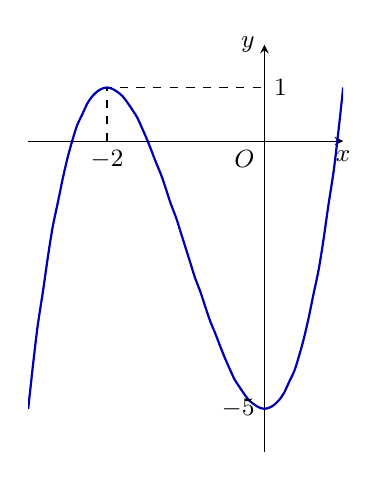
\begin{tikzpicture}[x=1cm,y=0.68cm,>=stealth,font=\small]
\draw[->] (-3,0)--(1,0) node[below]{$x$};
\draw[->] (0,-5.8)--(0,1.8) node[left]{$y$};
\node[below left] at (0,0){$O$};
\draw[dashed,thin] (-2,0)--(-2,1)--(0,1);
\begin{scope}\clip (-3,-5.81) rectangle (1,1.8);
\draw[thick,blue!70!black] plot[smooth] coordinates {(-3,-5) (-2.94,-4.19) (-2.88,-3.45) (-2.81,-2.78) (-2.75,-2.16) (-2.69,-1.61) (-2.62,-1.12) (-2.56,-0.69) (-2.5,-0.31) (-2.44,0.01) (-2.38,0.29) (-2.31,0.51) (-2.25,0.7) (-2.19,0.83) (-2.12,0.93) (-2.06,0.98) (-2,1) (-1.94,0.98) (-1.88,0.93) (-1.81,0.85) (-1.75,0.74) (-1.69,0.61) (-1.62,0.45) (-1.56,0.26) (-1.5,0.06) (-1.44,-0.16) (-1.38,-0.39) (-1.31,-0.64) (-1.25,-0.9) (-1.19,-1.17) (-1.12,-1.44) (-1.06,-1.72) (-1,-2) (-0.94,-2.28) (-0.88,-2.56) (-0.81,-2.83) (-0.75,-3.1) (-0.69,-3.36) (-0.62,-3.61) (-0.56,-3.84) (-0.5,-4.06) (-0.44,-4.26) (-0.38,-4.45) (-0.31,-4.61) (-0.25,-4.74) (-0.19,-4.85) (-0.12,-4.93) (-0.06,-4.98) (0,-5) (0.06,-4.98) (0.12,-4.93) (0.19,-4.83) (0.25,-4.7) (0.31,-4.51) (0.38,-4.29) (0.44,-4.01) (0.5,-3.69) (0.56,-3.31) (0.62,-2.88) (0.69,-2.39) (0.75,-1.84) (0.81,-1.22) (0.88,-0.55) (0.94,0.19) (1,1)};
\end{scope}
\node[below] at (-2,0){$-2$};
\node[left] at (0,-5){$-5$};
\node[right] at (0,1){$1$};
\end{tikzpicture}
\end{center}
Phương trình $f(x)=-7$ có bao nhiêu nghiệm thực?}{1}

\cauTLN[id=C1-B4-D04-NB-054,muc=NB,loigiai={Ta có $-2f(x)-4=0\Leftrightarrow f(x)=-2$. Số nghiệm bằng số giao điểm của đồ thị $y=f(x)$ với đường thẳng $y=-2$. Vậy có $1$ nghiệm.}]{Cho hàm số $y=f(x)$ có bảng biến thiên như sau:
\begin{center}

\begin{tikzpicture}
\tkzTabInit[lgt=1.2,espcl=1.9]{$x$/0.7,$y'$/0.7,$y$/2}{$-\infty$,$-3$,$-1$,$+\infty$}
\tkzTabLine{ ,-,z,+,z,-, }
\tkzTabVar{+/$+\infty$,-/$-1$,+/$1$,-/$-\infty$}
\end{tikzpicture}
\end{center}
Phương trình $-2f(x)-4=0$ có bao nhiêu nghiệm thực?}{1}

\cauTLN[id=C1-B4-D04-NB-055,muc=NB,loigiai={Ta có $3f(x)-6=0\Leftrightarrow f(x)=2$. Số nghiệm bằng số giao điểm của đồ thị $y=f(x)$ với đường thẳng $y=2$. Vậy có $2$ nghiệm.}]{Cho hàm số $y=f(x)$ có bảng biến thiên như sau:
\begin{center}

\begin{tikzpicture}
\tkzTabInit[lgt=1.2,espcl=1.9]{$x$/0.7,$y'$/0.7,$y$/2}{$-\infty$,$0$,$3$,$+\infty$}
\tkzTabLine{ ,-,z,+,z,-, }
\tkzTabVar{+/$+\infty$,-/$-4$,+/$2$,-/$-\infty$}
\end{tikzpicture}
\end{center}
Phương trình $3f(x)-6=0$ có bao nhiêu nghiệm thực?}{2}

\cauTLN[id=C1-B4-D04-NB-056,muc=NB,loigiai={Ta có $-2f(x)=0\Leftrightarrow f(x)=0$. Số nghiệm bằng số giao điểm của đồ thị $y=f(x)$ với đường thẳng $y=0$. Vậy có $2$ nghiệm.}]{Cho hàm số $y=f(x)$ xác định trên $\mathbb{R}\setminus\{-1\}$ và có bảng biến thiên như sau:
\begin{center}

\begin{tikzpicture}
\tkzTabInit[lgt=1.2,espcl=1.9]{$x$/0.7,$y'$/0.7,$y$/2}{$-\infty$,$-2$,$-1$,$0$,$+\infty$}
\tkzTabLine{ ,+,z,-,d,-,z,+, }
\tkzTabVar{-/$-\infty$,+/$1$,-D+/$-\infty$/$+\infty$,-/$5$,+/$+\infty$}
\end{tikzpicture}
\end{center}
Phương trình $-2f(x)=0$ có bao nhiêu nghiệm thực?}{2}

\cauTLN[id=C1-B4-D04-NB-057,muc=NB,loigiai={Số nghiệm của phương trình $f(x)=-3$ bằng số giao điểm của đồ thị $y=f(x)$ với đường thẳng $y=-3$. Vậy có $1$ nghiệm.}]{Cho hàm số $y=f(x)$ có đồ thị như hình vẽ.
\begin{center}
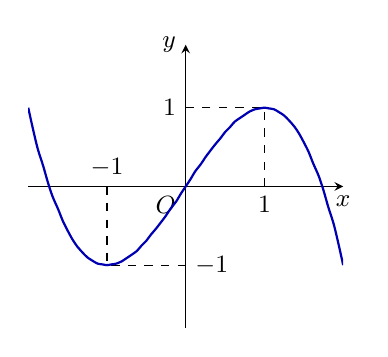
\begin{tikzpicture}[x=1cm,y=1cm,>=stealth,font=\small]
\draw[->] (-2,0)--(2,0) node[below]{$x$};
\draw[->] (0,-1.8)--(0,1.8) node[left]{$y$};
\node[below left] at (0,0){$O$};
\draw[dashed,thin] (-1,0)--(-1,-1)--(0,-1);
\draw[dashed,thin] (1,0)--(1,1)--(0,1);
\begin{scope}\clip (-2,-1.81) rectangle (2,1.8);
\draw[thick,blue!70!black] plot[smooth] coordinates {(-2,1) (-1.94,0.73) (-1.88,0.48) (-1.81,0.26) (-1.75,0.05) (-1.69,-0.13) (-1.62,-0.29) (-1.56,-0.44) (-1.5,-0.56) (-1.44,-0.67) (-1.38,-0.76) (-1.31,-0.84) (-1.25,-0.9) (-1.19,-0.94) (-1.12,-0.98) (-1.06,-0.99) (-1,-1) (-0.94,-0.99) (-0.88,-0.98) (-0.81,-0.95) (-0.75,-0.91) (-0.69,-0.87) (-0.62,-0.82) (-0.56,-0.75) (-0.5,-0.69) (-0.44,-0.61) (-0.38,-0.54) (-0.31,-0.45) (-0.25,-0.37) (-0.19,-0.28) (-0.12,-0.19) (-0.06,-0.09) (0,0) (0.06,0.09) (0.12,0.19) (0.19,0.28) (0.25,0.37) (0.31,0.45) (0.38,0.54) (0.44,0.61) (0.5,0.69) (0.56,0.75) (0.62,0.82) (0.69,0.87) (0.75,0.91) (0.81,0.95) (0.88,0.98) (0.94,0.99) (1,1) (1.06,0.99) (1.12,0.98) (1.19,0.94) (1.25,0.9) (1.31,0.84) (1.38,0.76) (1.44,0.67) (1.5,0.56) (1.56,0.44) (1.62,0.29) (1.69,0.13) (1.75,-0.05) (1.81,-0.26) (1.88,-0.48) (1.94,-0.73) (2,-1)};
\end{scope}
\node[above] at (-1,0){$-1$};
\node[below] at (1,0){$1$};
\node[right] at (0,-1){$-1$};
\node[left] at (0,1){$1$};
\end{tikzpicture}
\end{center}
Phương trình $f(x)=-3$ có bao nhiêu nghiệm thực?}{1}

\cauTLN[id=C1-B4-D04-NB-058,muc=NB,loigiai={Ta có $-2f(x)-8=0\Leftrightarrow f(x)=-4$. Số nghiệm bằng số giao điểm của đồ thị $y=f(x)$ với đường thẳng $y=-4$. Vậy có $2$ nghiệm.}]{Cho hàm số $y=f(x)$ có bảng biến thiên như sau:
\begin{center}

\begin{tikzpicture}
\tkzTabInit[lgt=1.2,espcl=1.9]{$x$/0.7,$y'$/0.7,$y$/2}{$-\infty$,$-2$,$0$,$+\infty$}
\tkzTabLine{ ,+,z,-,z,+, }
\tkzTabVar{-/$-\infty$,+/$4$,-/$-4$,+/$+\infty$}
\end{tikzpicture}
\end{center}
Phương trình $-2f(x)-8=0$ có bao nhiêu nghiệm thực?}{2}

\cauTLN[id=C1-B4-D04-NB-059,muc=NB,loigiai={Số nghiệm của phương trình $f(x)=4$ bằng số giao điểm của đồ thị $y=f(x)$ với đường thẳng $y=4$. Vậy có $1$ nghiệm.}]{Cho hàm số $y=f(x)$ có bảng biến thiên như sau:
\begin{center}

\begin{tikzpicture}
\tkzTabInit[lgt=1.2,espcl=1.9]{$x$/0.7,$y'$/0.7,$y$/2}{$-\infty$,$-3$,$-1$,$+\infty$}
\tkzTabLine{ ,-,z,+,z,-, }
\tkzTabVar{+/$+\infty$,-/$-5$,+/$3$,-/$-\infty$}
\end{tikzpicture}
\end{center}
Phương trình $f(x)=4$ có bao nhiêu nghiệm thực?}{1}

\cauTLN[id=C1-B4-D04-NB-060,muc=NB,loigiai={Số nghiệm của phương trình $f(x)=-3$ bằng số giao điểm của đồ thị $y=f(x)$ với đường thẳng $y=-3$. Vậy có $2$ nghiệm.}]{Cho hàm số $y=f(x)$ có bảng biến thiên như sau:
\begin{center}

\begin{tikzpicture}
\tkzTabInit[lgt=1.2,espcl=1.9]{$x$/0.7,$y'$/0.7,$y$/2}{$-\infty$,$-2$,$0$,$+\infty$}
\tkzTabLine{ ,-,z,+,z,-, }
\tkzTabVar{+/$+\infty$,-/$-3$,+/$3$,-/$-\infty$}
\end{tikzpicture}
\end{center}
Phương trình $f(x)=-3$ có bao nhiêu nghiệm thực?}{2}

\cauTN[id=C1-B4-D04-TH-001,muc=TH,loigiai={Phương trình hoành độ giao điểm: $-x^{3}-x^{2}+8x+11=-x+2\Leftrightarrow -x^{3}-x^{2}+9x+9=0\Leftrightarrow x=-3 \vee x=-1 \vee x=3$. Các giao điểm: $(-3;5)$, $(-1;3)$, $(3;-1)$.}]{Cho hàm số $y=-x^{3}-x^{2}+8x+11$ có đồ thị $(C)$ và đường thẳng $d: y=-x+2$. Điểm nào dưới đây là một giao điểm của $(C)$ và $d$?}
  {$(3;-1)$.}
  {$(3;0)$.}{$(-3;-1)$.}{$(4;-1)$.}

\cauTN[id=C1-B4-D04-TH-002,muc=TH,loigiai={Số nghiệm của phương trình $f(x)=-6$ bằng số giao điểm của đồ thị $y=f(x)$ với đường thẳng $y=-6$. Dựa vào bảng biến thiên ta được $1$ nghiệm.}]{Cho hàm số $y=f(x)$ xác định trên $\mathbb{R}\setminus\{0\}$ và có bảng biến thiên như sau:
\begin{center}

\begin{tikzpicture}
\tkzTabInit[lgt=1.2,espcl=1.9]{$x$/0.7,$y'$/0.7,$y$/2}{$-\infty$,$-1$,$0$,$1$,$+\infty$}
\tkzTabLine{ ,-,z,+,d,+,z,-, }
\tkzTabVar{+/$+\infty$,-/$-2$,+D-/$+\infty$/$-\infty$,+/$-6$,-/$-\infty$}
\end{tikzpicture}
\end{center}
Số nghiệm thực của phương trình $f(x)=-6$ là}
  {$1$.}
  {$2$.}{$0$.}{$3$.}

\cauTN[id=C1-B4-D04-TH-003,muc=TH,loigiai={Phương trình hoành độ giao điểm: $-x^{3}+4x^{2}-2x-3=x-3\Leftrightarrow -x^{3}+4x^{2}-3x=0\Leftrightarrow x=0 \vee x=1 \vee x=3$. Các giao điểm: $(0;-3)$, $(1;-2)$, $(3;0)$.}]{Cho hàm số $y=-x^{3}+4x^{2}-2x-3$ có đồ thị $(C)$ và đường thẳng $d: y=x-3$. Điểm nào dưới đây là một giao điểm của $(C)$ và $d$?}
  {$(3;0)$.}
  {$(0;3)$.}{$(3;1)$.}{$(-3;0)$.}

\cauTN[id=C1-B4-D04-TH-004,muc=TH,loigiai={Phương trình hoành độ giao điểm: $x^{3}+2x^{2}+3x-3=2x-3\Leftrightarrow x^{3}+2x^{2}+x=0\Leftrightarrow x=-1 \vee x=0$. Các giao điểm: $(-1;-5)$, $(0;-3)$.}]{Cho hàm số $y=x^{3}+2x^{2}+3x-3$ có đồ thị $(C)$ và đường thẳng $d: y=2x-3$. Điểm nào dưới đây là một giao điểm của $(C)$ và $d$?}
  {$(-1;-5)$.}
  {$(-5;-1)$.}{$(-1;-4)$.}{$(1;-5)$.}

\cauTN[id=C1-B4-D04-TH-005,muc=TH,loigiai={Phương trình hoành độ giao điểm: $x^{3}+x^{2}+1=2x+1\Leftrightarrow x^{3}+x^{2}-2x=0\Leftrightarrow x=-2 \vee x=0 \vee x=1$. Các giao điểm: $(-2;-3)$, $(0;1)$, $(1;3)$.}]{Cho hàm số $y=x^{3}+x^{2}+1$ có đồ thị $(C)$ và đường thẳng $d: y=2x+1$. Điểm nào dưới đây là một giao điểm của $(C)$ và $d$?}
  {$(-2;-3)$.}
  {$(-3;-2)$.}{$(-2;-2)$.}{$(2;-3)$.}

\cauTN[id=C1-B4-D04-TH-006,muc=TH,loigiai={Ta có $|f(x)|=6\Leftrightarrow f(x)=6$ hoặc $f(x)=-6$. Từ bảng biến thiên, phương trình $f(x)=6$ có $1$ nghiệm, phương trình $f(x)=-6$ có $1$ nghiệm (các nghiệm này khác nhau). Dựa vào bảng biến thiên ta được $2$ nghiệm.}]{Cho hàm số $y=f(x)$ có bảng biến thiên như sau:
\begin{center}

\begin{tikzpicture}
\tkzTabInit[lgt=1.2,espcl=1.9]{$x$/0.7,$y'$/0.7,$y$/2}{$-\infty$,$-2$,$0$,$+\infty$}
\tkzTabLine{ ,-,z,+,z,-, }
\tkzTabVar{+/$+\infty$,-/$-1$,+/$5$,-/$-\infty$}
\end{tikzpicture}
\end{center}
Số nghiệm thực của phương trình $|f(x)|=6$ là}
  {$2$.}
  {$3$.}{$1$.}{$4$.}

\cauTN[id=C1-B4-D04-TH-007,muc=TH,loigiai={Ta có $3f(x)+12=0\Leftrightarrow f(x)=-4$. Số nghiệm bằng số giao điểm của đồ thị $y=f(x)$ với đường thẳng $y=-4$. Dựa vào đồ thị ta được $1$ nghiệm.}]{Cho hàm số $y=f(x)$ có đồ thị như hình vẽ.
\begin{center}
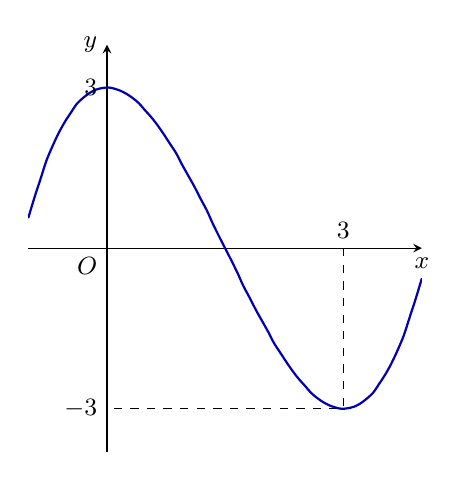
\begin{tikzpicture}[x=1cm,y=0.68cm,>=stealth,font=\small]
\draw[->] (-1,0)--(4,0) node[below]{$x$};
\draw[->] (0,-3.8)--(0,3.8) node[left]{$y$};
\node[below left] at (0,0){$O$};
\draw[dashed,thin] (3,0)--(3,-3)--(0,-3);
\begin{scope}\clip (-1,-3.81) rectangle (4,3.8);
\draw[thick,blue!70!black] plot[smooth] coordinates {(-1,0.56) (-0.92,0.95) (-0.84,1.31) (-0.77,1.63) (-0.69,1.91) (-0.61,2.16) (-0.53,2.37) (-0.45,2.55) (-0.38,2.7) (-0.3,2.81) (-0.22,2.9) (-0.14,2.96) (-0.06,2.99) (0.02,3) (0.09,2.98) (0.17,2.94) (0.25,2.88) (0.33,2.8) (0.41,2.7) (0.48,2.58) (0.56,2.45) (0.64,2.3) (0.72,2.13) (0.8,1.95) (0.88,1.77) (0.95,1.57) (1.03,1.36) (1.11,1.15) (1.19,0.92) (1.27,0.7) (1.34,0.47) (1.42,0.23) (1.5,0) (1.58,-0.23) (1.66,-0.47) (1.73,-0.7) (1.81,-0.92) (1.89,-1.15) (1.97,-1.36) (2.05,-1.57) (2.12,-1.77) (2.2,-1.95) (2.28,-2.13) (2.36,-2.3) (2.44,-2.45) (2.52,-2.58) (2.59,-2.7) (2.67,-2.8) (2.75,-2.88) (2.83,-2.94) (2.91,-2.98) (2.98,-3) (3.06,-2.99) (3.14,-2.96) (3.22,-2.9) (3.3,-2.81) (3.38,-2.7) (3.45,-2.55) (3.53,-2.37) (3.61,-2.16) (3.69,-1.91) (3.77,-1.63) (3.84,-1.31) (3.92,-0.95) (4,-0.56)};
\end{scope}
\node[above] at (3,0){$3$};
\node[left] at (0,-3){$-3$};
\node[left] at (0,3){$3$};
\end{tikzpicture}
\end{center}
Số nghiệm thực của phương trình $3f(x)+12=0$ là}
  {$1$.}
  {$2$.}{$0$.}{$3$.}

\cauTN[id=C1-B4-D04-TH-008,muc=TH,loigiai={Ta có $|f(x)|=5\Leftrightarrow f(x)=5$ hoặc $f(x)=-5$. Từ bảng biến thiên, phương trình $f(x)=5$ có $1$ nghiệm, phương trình $f(x)=-5$ có $2$ nghiệm (các nghiệm này khác nhau). Dựa vào bảng biến thiên ta được $3$ nghiệm.}]{Cho hàm số $y=f(x)$ xác định trên $\mathbb{R}\setminus\{1\}$ và có bảng biến thiên như sau:
\begin{center}

\begin{tikzpicture}
\tkzTabInit[lgt=1.2,espcl=1.9]{$x$/0.7,$y'$/0.7,$y$/2}{$-\infty$,$-1$,$1$,$3$,$+\infty$}
\tkzTabLine{ ,+,z,-,d,-,z,+, }
\tkzTabVar{-/$-\infty$,+/$-3$,-D+/$-\infty$/$+\infty$,-/$5$,+/$+\infty$}
\end{tikzpicture}
\end{center}
Số nghiệm thực của phương trình $|f(x)|=5$ là}
  {$3$.}
  {$4$.}{$2$.}{$5$.}

\cauTN[id=C1-B4-D04-TH-009,muc=TH,loigiai={Phương trình hoành độ giao điểm: $-x^{3}-x^{2}+x+3=-x+3\Leftrightarrow -x^{3}-x^{2}+2x=0\Leftrightarrow x=-2 \vee x=0 \vee x=1$. Các giao điểm: $(-2;5)$, $(0;3)$, $(1;2)$.}]{Cho hàm số $y=-x^{3}-x^{2}+x+3$ có đồ thị $(C)$ và đường thẳng $d: y=-x+3$. Tổng hoành độ các giao điểm của $(C)$ và $d$ bằng}
  {$-1$.}
  {$1$.}{$-3$.}{$-5$.}

\cauTN[id=C1-B4-D04-TH-010,muc=TH,loigiai={Phương trình hoành độ giao điểm: $-x^{3}-2x^{2}+5x+6=x-2\Leftrightarrow -x^{3}-2x^{2}+4x+8=0\Leftrightarrow x=-2 \vee x=2$. Các giao điểm: $(-2;-4)$, $(2;0)$.}]{Cho hàm số $y=-x^{3}-2x^{2}+5x+6$ có đồ thị $(C)$ và đường thẳng $d: y=x-2$. Số giao điểm của $(C)$ và $d$ là}
  {$2$.}
  {$3$.}{$1$.}{$0$.}

\cauTN[id=C1-B4-D04-TH-011,muc=TH,loigiai={Phương trình hoành độ giao điểm: $x^{3}+4x^{2}+2x=-2x\Leftrightarrow x^{3}+4x^{2}+4x=0\Leftrightarrow x=-2 \vee x=0$. Các giao điểm: $(-2;4)$, $(0;0)$.}]{Cho hàm số $y=x^{3}+4x^{2}+2x$ có đồ thị $(C)$ và đường thẳng $d: y=-2x$. Tổng hoành độ các giao điểm của $(C)$ và $d$ bằng}
  {$-2$.}
  {$0$.}{$2$.}{$-3$.}

\cauTN[id=C1-B4-D04-TH-012,muc=TH,loigiai={Ta có $2f(x)+4=0\Leftrightarrow f(x)=-2$. Số nghiệm bằng số giao điểm của đồ thị $y=f(x)$ với đường thẳng $y=-2$. Dựa vào bảng biến thiên ta được $3$ nghiệm.}]{Cho hàm số $y=f(x)$ có bảng biến thiên như sau:
\begin{center}

\begin{tikzpicture}
\tkzTabInit[lgt=1.2,espcl=1.9]{$x$/0.7,$y'$/0.7,$y$/2}{$-\infty$,$-3$,$-1$,$+\infty$}
\tkzTabLine{ ,-,z,+,z,-, }
\tkzTabVar{+/$+\infty$,-/$-3$,+/$-1$,-/$-\infty$}
\end{tikzpicture}
\end{center}
Số nghiệm thực của phương trình $2f(x)+4=0$ là}
  {$3$.}
  {$4$.}{$2$.}{$5$.}

\cauTN[id=C1-B4-D04-TH-013,muc=TH,loigiai={Phương trình hoành độ giao điểm: $-x^{3}+x^{2}-2x-1=-2x-1\Leftrightarrow -x^{3}+x^{2}=0\Leftrightarrow x=0 \vee x=1$. Các giao điểm: $(0;-1)$, $(1;-3)$.}]{Cho hàm số $y=-x^{3}+x^{2}-2x-1$ có đồ thị $(C)$ và đường thẳng $d: y=-2x-1$. Điểm nào dưới đây là một giao điểm của $(C)$ và $d$?}
  {$(1;-3)$.}
  {$(-3;1)$.}{$(1;-2)$.}{$(-1;-3)$.}

\cauTN[id=C1-B4-D04-TH-014,muc=TH,loigiai={Phương trình hoành độ giao điểm: $x^{3}-4x^{2}-2x+15=x-3\Leftrightarrow x^{3}-4x^{2}-3x+18=0\Leftrightarrow x=-2 \vee x=3$. Các giao điểm: $(-2;-5)$, $(3;0)$.}]{Cho hàm số $y=x^{3}-4x^{2}-2x+15$ có đồ thị $(C)$ và đường thẳng $d: y=x-3$. Số giao điểm của $(C)$ và $d$ là}
  {$2$.}
  {$3$.}{$1$.}{$0$.}

\cauTN[id=C1-B4-D04-TH-015,muc=TH,loigiai={Ta có $2f(x)=0\Leftrightarrow f(x)=0$. Số nghiệm bằng số giao điểm của đồ thị $y=f(x)$ với đường thẳng $y=0$. Dựa vào bảng biến thiên ta được $2$ nghiệm.}]{Cho hàm số $y=f(x)$ có bảng biến thiên như sau:
\begin{center}

\begin{tikzpicture}
\tkzTabInit[lgt=1.2,espcl=1.9]{$x$/0.7,$y'$/0.7,$y$/2}{$-\infty$,$-3$,$-1$,$+\infty$}
\tkzTabLine{ ,-,z,+,z,-, }
\tkzTabVar{+/$+\infty$,-/$0$,+/$4$,-/$-\infty$}
\end{tikzpicture}
\end{center}
Số nghiệm thực của phương trình $2f(x)=0$ là}
  {$2$.}
  {$3$.}{$1$.}{$4$.}

\cauTN[id=C1-B4-D04-TH-016,muc=TH,loigiai={Ta có $3f(x)-18=0\Leftrightarrow f(x)=6$. Số nghiệm bằng số giao điểm của đồ thị $y=f(x)$ với đường thẳng $y=6$. Dựa vào bảng biến thiên ta được $1$ nghiệm.}]{Cho hàm số $y=f(x)$ có bảng biến thiên như sau:
\begin{center}

\begin{tikzpicture}
\tkzTabInit[lgt=1.2,espcl=1.9]{$x$/0.7,$y'$/0.7,$y$/2}{$-\infty$,$1$,$3$,$+\infty$}
\tkzTabLine{ ,+,z,-,z,+, }
\tkzTabVar{-/$-\infty$,+/$4$,-/$0$,+/$+\infty$}
\end{tikzpicture}
\end{center}
Số nghiệm thực của phương trình $3f(x)-18=0$ là}
  {$1$.}
  {$2$.}{$0$.}{$3$.}

\cauTN[id=C1-B4-D04-TH-017,muc=TH,loigiai={Phương trình hoành độ giao điểm: $-x^{3}-2x^{2}+5x+8=2\Leftrightarrow -x^{3}-2x^{2}+5x+6=0\Leftrightarrow x=-3 \vee x=-1 \vee x=2$. Các giao điểm: $(-3;2)$, $(-1;2)$, $(2;2)$.}]{Cho hàm số $y=-x^{3}-2x^{2}+5x+8$ có đồ thị $(C)$ và đường thẳng $d: y=2$. Số giao điểm của $(C)$ và $d$ là}
  {$3$.}
  {$2$.}{$1$.}{$0$.}

\cauTN[id=C1-B4-D04-TH-018,muc=TH,loigiai={Phương trình hoành độ giao điểm: $-x^{3}-5x^{2}-8x-2=-x+1\Leftrightarrow -x^{3}-5x^{2}-7x-3=0\Leftrightarrow x=-3 \vee x=-1$. Các giao điểm: $(-3;4)$, $(-1;2)$.}]{Cho hàm số $y=-x^{3}-5x^{2}-8x-2$ có đồ thị $(C)$ và đường thẳng $d: y=-x+1$. Điểm nào dưới đây là một giao điểm của $(C)$ và $d$?}
  {$(-3;4)$.}
  {$(4;-3)$.}{$(-3;5)$.}{$(3;4)$.}

\cauTN[id=C1-B4-D04-TH-019,muc=TH,loigiai={Ta có $2f(x)+8=0\Leftrightarrow f(x)=-4$. Số nghiệm bằng số giao điểm của đồ thị $y=f(x)$ với đường thẳng $y=-4$. Dựa vào bảng biến thiên ta được $1$ nghiệm.}]{Cho hàm số $y=f(x)$ có bảng biến thiên như sau:
\begin{center}

\begin{tikzpicture}
\tkzTabInit[lgt=1.2,espcl=1.9]{$x$/0.7,$y'$/0.7,$y$/2}{$-\infty$,$-2$,$0$,$+\infty$}
\tkzTabLine{ ,+,z,-,z,+, }
\tkzTabVar{-/$-\infty$,+/$0$,-/$-2$,+/$+\infty$}
\end{tikzpicture}
\end{center}
Số nghiệm thực của phương trình $2f(x)+8=0$ là}
  {$1$.}
  {$2$.}{$0$.}{$3$.}

\cauTN[id=C1-B4-D04-TH-020,muc=TH,loigiai={Ta có $|f(x)|=1\Leftrightarrow f(x)=1$ hoặc $f(x)=-1$. Từ đồ thị, phương trình $f(x)=1$ có $2$ nghiệm, phương trình $f(x)=-1$ có $2$ nghiệm (các nghiệm này khác nhau). Dựa vào đồ thị ta được $4$ nghiệm.}]{Cho hàm số $y=f(x)$ có đồ thị như hình vẽ.
\begin{center}
\begin{tikzpicture}[x=1cm,y=1cm,>=stealth,font=\small]
\draw[->] (-3,0)--(3,0) node[below]{$x$};
\draw[->] (0,-1.8)--(0,1.8) node[left]{$y$};
\node[below left] at (0,0){$O$};
\draw[dashed,thin] (-2,0)--(-2,1)--(0,1);
\draw[dashed,thin] (2,0)--(2,-1)--(0,-1);
\begin{scope}\clip (-3,-1.81) rectangle (3,1.8);
\draw[thick,blue!70!black] plot[smooth] coordinates {(-3,0.56) (-2.91,0.65) (-2.81,0.72) (-2.72,0.78) (-2.62,0.84) (-2.53,0.88) (-2.44,0.92) (-2.34,0.95) (-2.25,0.98) (-2.16,0.99) (-2.06,1) (-1.97,1) (-1.88,0.99) (-1.78,0.98) (-1.69,0.97) (-1.59,0.94) (-1.5,0.91) (-1.41,0.88) (-1.31,0.84) (-1.22,0.8) (-1.12,0.75) (-1.03,0.7) (-0.94,0.65) (-0.84,0.6) (-0.75,0.54) (-0.66,0.47) (-0.56,0.41) (-0.47,0.35) (-0.38,0.28) (-0.28,0.21) (-0.19,0.14) (-0.09,0.07) (0,0) (0.09,-0.07) (0.19,-0.14) (0.28,-0.21) (0.38,-0.28) (0.47,-0.35) (0.56,-0.41) (0.66,-0.47) (0.75,-0.54) (0.84,-0.6) (0.94,-0.65) (1.03,-0.7) (1.12,-0.75) (1.22,-0.8) (1.31,-0.84) (1.41,-0.88) (1.5,-0.91) (1.59,-0.94) (1.69,-0.97) (1.78,-0.98) (1.88,-0.99) (1.97,-1) (2.06,-1) (2.16,-0.99) (2.25,-0.98) (2.34,-0.95) (2.44,-0.92) (2.53,-0.88) (2.62,-0.84) (2.72,-0.78) (2.81,-0.72) (2.91,-0.65) (3,-0.56)};
\end{scope}
\node[below] at (-2,0){$-2$};
\node[above] at (2,0){$2$};
\node[left] at (0,-1){$-1$};
\node[right] at (0,1){$1$};
\end{tikzpicture}
\end{center}
Số nghiệm thực của phương trình $|f(x)|=1$ là}
  {$4$.}
  {$5$.}{$3$.}{$6$.}

\cauTN[id=C1-B4-D04-TH-021,muc=TH,loigiai={Phương trình hoành độ giao điểm: $-x^{3}-6x^{2}-11x-6=0\Leftrightarrow -x^{3}-6x^{2}-11x-6=0\Leftrightarrow x=-3 \vee x=-2 \vee x=-1$. Các giao điểm: $(-3;0)$, $(-2;0)$, $(-1;0)$.}]{Cho hàm số $y=-x^{3}-6x^{2}-11x-6$ có đồ thị $(C)$ và đường thẳng $d: y=0$. Số giao điểm của $(C)$ và $d$ là}
  {$3$.}
  {$2$.}{$1$.}{$0$.}

\cauTN[id=C1-B4-D04-TH-022,muc=TH,loigiai={Phương trình hoành độ giao điểm: $-x^{3}+4x^{2}-4x+2=-x+2\Leftrightarrow -x^{3}+4x^{2}-3x=0\Leftrightarrow x=0 \vee x=1 \vee x=3$. Các giao điểm: $(0;2)$, $(1;1)$, $(3;-1)$.}]{Cho hàm số $y=-x^{3}+4x^{2}-4x+2$ có đồ thị $(C)$ và đường thẳng $d: y=-x+2$. Số giao điểm của $(C)$ và $d$ là}
  {$3$.}
  {$2$.}{$1$.}{$0$.}

\cauTN[id=C1-B4-D04-TH-023,muc=TH,loigiai={Phương trình hoành độ giao điểm: $-x^{3}+11x+1=2x+1\Leftrightarrow -x^{3}+9x=0\Leftrightarrow x=-3 \vee x=0 \vee x=3$. Các giao điểm: $(-3;-5)$, $(0;1)$, $(3;7)$.}]{Cho hàm số $y=-x^{3}+11x+1$ có đồ thị $(C)$ và đường thẳng $d: y=2x+1$. Điểm nào dưới đây là một giao điểm của $(C)$ và $d$?}
  {$(-3;-5)$.}
  {$(-5;-3)$.}{$(-3;-4)$.}{$(3;-5)$.}

\cauTN[id=C1-B4-D04-TH-024,muc=TH,loigiai={Ta có $2f(x)-10=0\Leftrightarrow f(x)=5$. Số nghiệm bằng số giao điểm của đồ thị $y=f(x)$ với đường thẳng $y=5$. Dựa vào bảng biến thiên ta được $1$ nghiệm.}]{Cho hàm số $y=f(x)$ có bảng biến thiên như sau:
\begin{center}

\begin{tikzpicture}
\tkzTabInit[lgt=1.2,espcl=1.9]{$x$/0.7,$y'$/0.7,$y$/2}{$-\infty$,$-3$,$-1$,$+\infty$}
\tkzTabLine{ ,+,z,-,z,+, }
\tkzTabVar{-/$-\infty$,+/$4$,-/$-4$,+/$+\infty$}
\end{tikzpicture}
\end{center}
Số nghiệm thực của phương trình $2f(x)-10=0$ là}
  {$1$.}
  {$2$.}{$0$.}{$3$.}

\cauTN[id=C1-B4-D04-TH-025,muc=TH,loigiai={Phương trình hoành độ giao điểm: $x^{3}-3x^{2}-x-2=-x-2\Leftrightarrow x^{3}-3x^{2}=0\Leftrightarrow x=0 \vee x=3$. Các giao điểm: $(0;-2)$, $(3;-5)$.}]{Cho hàm số $y=x^{3}-3x^{2}-x-2$ có đồ thị $(C)$ và đường thẳng $d: y=-x-2$. Tổng hoành độ các giao điểm của $(C)$ và $d$ bằng}
  {$3$.}
  {$6$.}{$1$.}{$2$.}

\cauTN[id=C1-B4-D04-TH-026,muc=TH,loigiai={Phương trình hoành độ giao điểm: $x^{3}-x^{2}+1=x\Leftrightarrow x^{3}-x^{2}-x+1=0\Leftrightarrow x=-1 \vee x=1$. Các giao điểm: $(-1;-1)$, $(1;1)$.}]{Cho hàm số $y=x^{3}-x^{2}+1$ có đồ thị $(C)$ và đường thẳng $d: y=x$. Tổng hoành độ các giao điểm của $(C)$ và $d$ bằng}
  {$0$.}
  {$1$.}{$4$.}{$-2$.}

\cauTN[id=C1-B4-D04-TH-027,muc=TH,loigiai={Số nghiệm của phương trình $f(x)=-5$ bằng số giao điểm của đồ thị $y=f(x)$ với đường thẳng $y=-5$. Dựa vào đồ thị ta được $1$ nghiệm.}]{Cho hàm số $y=f(x)$ có đồ thị như hình vẽ.
\begin{center}
\begin{tikzpicture}[x=1cm,y=0.54cm,>=stealth,font=\small]
\draw[->] (-3,0)--(3,0) node[below]{$x$};
\draw[->] (0,-3.8)--(0,5.8) node[left]{$y$};
\node[below left] at (0,0){$O$};
\draw[dashed,thin] (-2,0)--(-2,-3)--(0,-3);
\draw[dashed,thin] (2,0)--(2,5)--(0,5);
\begin{scope}\clip (-3,-3.81) rectangle (3,5.8);
\draw[thick,blue!70!black] plot[smooth] coordinates {(-3,-1.25) (-2.91,-1.58) (-2.81,-1.88) (-2.72,-2.13) (-2.62,-2.35) (-2.53,-2.54) (-2.44,-2.69) (-2.34,-2.81) (-2.25,-2.9) (-2.16,-2.96) (-2.06,-2.99) (-1.97,-3) (-1.88,-2.98) (-1.78,-2.93) (-1.69,-2.86) (-1.59,-2.77) (-1.5,-2.66) (-1.41,-2.52) (-1.31,-2.37) (-1.22,-2.2) (-1.12,-2.02) (-1.03,-1.82) (-0.94,-1.61) (-0.84,-1.38) (-0.75,-1.14) (-0.66,-0.9) (-0.56,-0.64) (-0.47,-0.38) (-0.38,-0.11) (-0.28,0.16) (-0.19,0.44) (-0.09,0.72) (0,1) (0.09,1.28) (0.19,1.56) (0.28,1.84) (0.38,2.11) (0.47,2.38) (0.56,2.64) (0.66,2.9) (0.75,3.14) (0.84,3.38) (0.94,3.61) (1.03,3.82) (1.12,4.02) (1.22,4.2) (1.31,4.37) (1.41,4.52) (1.5,4.66) (1.59,4.77) (1.69,4.86) (1.78,4.93) (1.88,4.98) (1.97,5) (2.06,4.99) (2.16,4.96) (2.25,4.9) (2.34,4.81) (2.44,4.69) (2.53,4.54) (2.62,4.35) (2.72,4.13) (2.81,3.88) (2.91,3.58) (3,3.25)};
\end{scope}
\node[above] at (-2,0){$-2$};
\node[below] at (2,0){$2$};
\node[right] at (0,-3){$-3$};
\node[left] at (0,5){$5$};
\end{tikzpicture}
\end{center}
Số nghiệm thực của phương trình $f(x)=-5$ là}
  {$1$.}
  {$2$.}{$0$.}{$3$.}

\cauTN[id=C1-B4-D04-TH-028,muc=TH,loigiai={Phương trình hoành độ giao điểm: $x^{3}-8x+3=x+3\Leftrightarrow x^{3}-9x=0\Leftrightarrow x=-3 \vee x=0 \vee x=3$. Các giao điểm: $(-3;0)$, $(0;3)$, $(3;6)$.}]{Cho hàm số $y=x^{3}-8x+3$ có đồ thị $(C)$ và đường thẳng $d: y=x+3$. Tổng hoành độ các giao điểm của $(C)$ và $d$ bằng}
  {$0$.}
  {$3$.}{$2$.}{$-2$.}

\cauTN[id=C1-B4-D04-TH-029,muc=TH,loigiai={Ta có $|f(x)|=1\Leftrightarrow f(x)=1$ hoặc $f(x)=-1$. Từ bảng biến thiên, phương trình $f(x)=1$ có $1$ nghiệm, phương trình $f(x)=-1$ có $3$ nghiệm (các nghiệm này khác nhau). Dựa vào bảng biến thiên ta được $4$ nghiệm.}]{Cho hàm số $y=f(x)$ có bảng biến thiên như sau:
\begin{center}

\begin{tikzpicture}
\tkzTabInit[lgt=1.2,espcl=1.9]{$x$/0.7,$y'$/0.7,$y$/2}{$-\infty$,$0$,$2$,$+\infty$}
\tkzTabLine{ ,+,z,-,z,+, }
\tkzTabVar{-/$-\infty$,+/$0$,-/$-2$,+/$+\infty$}
\end{tikzpicture}
\end{center}
Số nghiệm thực của phương trình $|f(x)|=1$ là}
  {$4$.}
  {$5$.}{$3$.}{$6$.}

\cauTN[id=C1-B4-D04-TH-030,muc=TH,loigiai={Ta có $-2f(x)+4=0\Leftrightarrow f(x)=2$. Số nghiệm bằng số giao điểm của đồ thị $y=f(x)$ với đường thẳng $y=2$. Dựa vào bảng biến thiên ta được $1$ nghiệm.}]{Cho hàm số $y=f(x)$ có bảng biến thiên như sau:
\begin{center}

\begin{tikzpicture}
\tkzTabInit[lgt=1.2,espcl=1.9]{$x$/0.7,$y'$/0.7,$y$/2}{$-\infty$,$0$,$3$,$+\infty$}
\tkzTabLine{ ,+,z,-,z,+, }
\tkzTabVar{-/$-\infty$,+/$0$,-/$-3$,+/$+\infty$}
\end{tikzpicture}
\end{center}
Số nghiệm thực của phương trình $-2f(x)+4=0$ là}
  {$1$.}
  {$2$.}{$0$.}{$3$.}

\cauTN[id=C1-B4-D04-TH-031,muc=TH,loigiai={Số nghiệm của phương trình $f(x)=-1$ bằng số giao điểm của đồ thị $y=f(x)$ với đường thẳng $y=-1$. Dựa vào bảng biến thiên ta được $2$ nghiệm.}]{Cho hàm số $y=f(x)$ có bảng biến thiên như sau:
\begin{center}
\begin{tikzpicture}
\tkzTabInit[lgt=1.2,espcl=1.9]{$x$/0.7,$y'$/0.7,$y$/2}{$-\infty$,$-3$,$-1$,$+\infty$}
\tkzTabLine{ ,+,z,-,z,+, }
\tkzTabVar{-/$-\infty$,+/$5$,-/$-1$,+/$+\infty$}
\end{tikzpicture}
\end{center}
Số nghiệm thực của phương trình $f(x)=-1$ là}
  {$2$.}
  {$3$.}{$1$.}{$4$.}

\cauTN[id=C1-B4-D04-TH-032,muc=TH,loigiai={Ta có $2f(x)-4=0\Leftrightarrow f(x)=2$. Số nghiệm bằng số giao điểm của đồ thị $y=f(x)$ với đường thẳng $y=2$. Dựa vào đồ thị ta được $1$ nghiệm.}]{Cho hàm số $y=f(x)$ có đồ thị như hình vẽ.
\begin{center}
\begin{tikzpicture}[x=1cm,y=0.93cm,>=stealth,font=\small]
\draw[->] (-3,0)--(3,0) node[below]{$x$};
\draw[->] (0,-4.8)--(0,0.8) node[left]{$y$};
\node[below left] at (0,0){$O$};
\draw[dashed,thin] (2,0)--(2,-4)--(0,-4);
\begin{scope}\clip (-3,-4.81) rectangle (3,0.8);
\draw[thick,blue!70!black] plot[smooth] coordinates {(-3,-0.88) (-2.91,-0.71) (-2.81,-0.56) (-2.72,-0.43) (-2.62,-0.32) (-2.53,-0.23) (-2.44,-0.15) (-2.34,-0.09) (-2.25,-0.05) (-2.16,-0.02) (-2.06,-0) (-1.97,-0) (-1.88,-0.01) (-1.78,-0.03) (-1.69,-0.07) (-1.59,-0.12) (-1.5,-0.17) (-1.41,-0.24) (-1.31,-0.31) (-1.22,-0.4) (-1.12,-0.49) (-1.03,-0.59) (-0.94,-0.7) (-0.84,-0.81) (-0.75,-0.93) (-0.66,-1.05) (-0.56,-1.18) (-0.47,-1.31) (-0.38,-1.44) (-0.28,-1.58) (-0.19,-1.72) (-0.09,-1.86) (0,-2) (0.09,-2.14) (0.19,-2.28) (0.28,-2.42) (0.38,-2.56) (0.47,-2.69) (0.56,-2.82) (0.66,-2.95) (0.75,-3.07) (0.84,-3.19) (0.94,-3.3) (1.03,-3.41) (1.12,-3.51) (1.22,-3.6) (1.31,-3.69) (1.41,-3.76) (1.5,-3.83) (1.59,-3.88) (1.69,-3.93) (1.78,-3.97) (1.88,-3.99) (1.97,-4) (2.06,-4) (2.16,-3.98) (2.25,-3.95) (2.34,-3.91) (2.44,-3.85) (2.53,-3.77) (2.62,-3.68) (2.72,-3.57) (2.81,-3.44) (2.91,-3.29) (3,-3.12)};
\end{scope}
\node[below] at (-2,0){$-2$};
\node[above] at (2,0){$2$};
\node[left] at (0,-4){$-4$};
\end{tikzpicture}
\end{center}
Số nghiệm thực của phương trình $2f(x)-4=0$ là}
  {$1$.}
  {$2$.}{$0$.}{$3$.}

\cauTN[id=C1-B4-D04-TH-033,muc=TH,loigiai={Ta có $|f(x)|=4\Leftrightarrow f(x)=4$ hoặc $f(x)=-4$. Từ đồ thị, phương trình $f(x)=4$ có $1$ nghiệm, phương trình $f(x)=-4$ có $2$ nghiệm (các nghiệm này khác nhau). Dựa vào đồ thị ta được $3$ nghiệm.}]{Cho hàm số $y=f(x)$ có đồ thị như hình vẽ.
\begin{center}
\begin{tikzpicture}[x=1cm,y=0.68cm,>=stealth,font=\small]
\draw[->] (-1,0)--(4,0) node[below]{$x$};
\draw[->] (0,-4.8)--(0,2.8) node[left]{$y$};
\node[below left] at (0,0){$O$};
\draw[dashed,thin] (3,0)--(3,-4)--(0,-4);
\begin{scope}\clip (-1,-4.81) rectangle (4,2.8);
\draw[thick,blue!70!black] plot[smooth] coordinates {(-1,-0.44) (-0.92,-0.05) (-0.84,0.31) (-0.77,0.63) (-0.69,0.91) (-0.61,1.16) (-0.53,1.37) (-0.45,1.55) (-0.38,1.7) (-0.3,1.81) (-0.22,1.9) (-0.14,1.96) (-0.06,1.99) (0.02,2) (0.09,1.98) (0.17,1.94) (0.25,1.88) (0.33,1.8) (0.41,1.7) (0.48,1.58) (0.56,1.45) (0.64,1.3) (0.72,1.13) (0.8,0.95) (0.88,0.77) (0.95,0.57) (1.03,0.36) (1.11,0.15) (1.19,-0.08) (1.27,-0.3) (1.34,-0.53) (1.42,-0.77) (1.5,-1) (1.58,-1.23) (1.66,-1.47) (1.73,-1.7) (1.81,-1.92) (1.89,-2.15) (1.97,-2.36) (2.05,-2.57) (2.12,-2.77) (2.2,-2.95) (2.28,-3.13) (2.36,-3.3) (2.44,-3.45) (2.52,-3.58) (2.59,-3.7) (2.67,-3.8) (2.75,-3.88) (2.83,-3.94) (2.91,-3.98) (2.98,-4) (3.06,-3.99) (3.14,-3.96) (3.22,-3.9) (3.3,-3.81) (3.38,-3.7) (3.45,-3.55) (3.53,-3.37) (3.61,-3.16) (3.69,-2.91) (3.77,-2.63) (3.84,-2.31) (3.92,-1.95) (4,-1.56)};
\end{scope}
\node[above] at (3,0){$3$};
\node[left] at (0,-4){$-4$};
\node[left] at (0,2){$2$};
\end{tikzpicture}
\end{center}
Số nghiệm thực của phương trình $|f(x)|=4$ là}
  {$3$.}
  {$4$.}{$2$.}{$5$.}

\cauTN[id=C1-B4-D04-TH-034,muc=TH,loigiai={Phương trình hoành độ giao điểm: $-x^{3}-x^{2}+x+1=x+1\Leftrightarrow -x^{3}-x^{2}=0\Leftrightarrow x=-1 \vee x=0$. Các giao điểm: $(-1;0)$, $(0;1)$.}]{Cho hàm số $y=-x^{3}-x^{2}+x+1$ có đồ thị $(C)$ và đường thẳng $d: y=x+1$. Số giao điểm của $(C)$ và $d$ là}
  {$2$.}
  {$3$.}{$1$.}{$0$.}

\cauTN[id=C1-B4-D04-TH-035,muc=TH,loigiai={Ta có $3f(x)+24=0\Leftrightarrow f(x)=-8$. Số nghiệm bằng số giao điểm của đồ thị $y=f(x)$ với đường thẳng $y=-8$. Dựa vào bảng biến thiên ta được $2$ nghiệm.}]{Cho hàm số $y=f(x)$ xác định trên $\mathbb{R}\setminus\{2\}$ và có bảng biến thiên như sau:
\begin{center}
\begin{tikzpicture}
\tkzTabInit[lgt=1.2,espcl=1.9]{$x$/0.7,$y'$/0.7,$y$/2}{$-\infty$,$1$,$2$,$3$,$+\infty$}
\tkzTabLine{ ,-,z,+,d,+,z,-, }
\tkzTabVar{+/$+\infty$,-/$-2$,+D-/$+\infty$/$-\infty$,+/$-6$,-/$-\infty$}
\end{tikzpicture}
\end{center}
Số nghiệm thực của phương trình $3f(x)+24=0$ là}
  {$2$.}
  {$3$.}{$1$.}{$4$.}

\cauTN[id=C1-B4-D04-TH-036,muc=TH,loigiai={Phương trình hoành độ giao điểm: $-x^{3}-x^{2}+5x+1=-x+1\Leftrightarrow -x^{3}-x^{2}+6x=0\Leftrightarrow x=-3 \vee x=0 \vee x=2$. Các giao điểm: $(-3;4)$, $(0;1)$, $(2;-1)$.}]{Cho hàm số $y=-x^{3}-x^{2}+5x+1$ có đồ thị $(C)$ và đường thẳng $d: y=-x+1$. Tổng hoành độ các giao điểm của $(C)$ và $d$ bằng}
  {$-1$.}
  {$2$.}{$1$.}{$0$.}

\cauTN[id=C1-B4-D04-TH-037,muc=TH,loigiai={Phương trình hoành độ giao điểm: $x^{3}-x^{2}+2x-1=2x-1\Leftrightarrow x^{3}-x^{2}=0\Leftrightarrow x=0 \vee x=1$. Các giao điểm: $(0;-1)$, $(1;1)$.}]{Cho hàm số $y=x^{3}-x^{2}+2x-1$ có đồ thị $(C)$ và đường thẳng $d: y=2x-1$. Tổng hoành độ các giao điểm của $(C)$ và $d$ bằng}
  {$1$.}
  {$3$.}{$5$.}{$2$.}

\cauTN[id=C1-B4-D04-TH-038,muc=TH,loigiai={Ta có $-2f(x)+12=0\Leftrightarrow f(x)=6$. Số nghiệm bằng số giao điểm của đồ thị $y=f(x)$ với đường thẳng $y=6$. Dựa vào bảng biến thiên ta được $1$ nghiệm.}]{Cho hàm số $y=f(x)$ xác định trên $\mathbb{R}\setminus\{0\}$ và có bảng biến thiên như sau:
\begin{center}
\begin{tikzpicture}
\tkzTabInit[lgt=1.2,espcl=1.9]{$x$/0.7,$y'$/0.7,$y$/2}{$-\infty$,$-1$,$0$,$1$,$+\infty$}
\tkzTabLine{ ,-,z,+,d,+,z,-, }
\tkzTabVar{+/$+\infty$,-/$6$,+D-/$+\infty$/$-\infty$,+/$2$,-/$-\infty$}
\end{tikzpicture}
\end{center}
Số nghiệm thực của phương trình $-2f(x)+12=0$ là}
  {$1$.}
  {$2$.}{$0$.}{$3$.}

\cauTN[id=C1-B4-D04-TH-039,muc=TH,loigiai={Phương trình hoành độ giao điểm: $-x^{3}-3x^{2}+4x+14=2\Leftrightarrow -x^{3}-3x^{2}+4x+12=0\Leftrightarrow x=-3 \vee x=-2 \vee x=2$. Các giao điểm: $(-3;2)$, $(-2;2)$, $(2;2)$.}]{Cho hàm số $y=-x^{3}-3x^{2}+4x+14$ có đồ thị $(C)$ và đường thẳng $d: y=2$. Tổng hoành độ các giao điểm của $(C)$ và $d$ bằng}
  {$-3$.}
  {$0$.}{$3$.}{$-5$.}

\cauTN[id=C1-B4-D04-TH-040,muc=TH,loigiai={Phương trình hoành độ giao điểm: $-x^{3}-4x^{2}-3x+9=-2x+3\Leftrightarrow -x^{3}-4x^{2}-x+6=0\Leftrightarrow x=-3 \vee x=-2 \vee x=1$. Các giao điểm: $(-3;9)$, $(-2;7)$, $(1;1)$.}]{Cho hàm số $y=-x^{3}-4x^{2}-3x+9$ có đồ thị $(C)$ và đường thẳng $d: y=-2x+3$. Điểm nào dưới đây là một giao điểm của $(C)$ và $d$?}
  {$(-3;9)$.}
  {$(9;-3)$.}{$(-3;10)$.}{$(3;9)$.}

\cauTN[id=C1-B4-D04-TH-041,muc=TH,loigiai={Phương trình hoành độ giao điểm: $-x^{3}+9x-9=2x-3\Leftrightarrow -x^{3}+7x-6=0\Leftrightarrow x=-3 \vee x=1 \vee x=2$. Các giao điểm: $(-3;-9)$, $(1;-1)$, $(2;1)$.}]{Cho hàm số $y=-x^{3}+9x-9$ có đồ thị $(C)$ và đường thẳng $d: y=2x-3$. Tổng hoành độ các giao điểm của $(C)$ và $d$ bằng}
  {$0$.}
  {$3$.}{$-1$.}{$-2$.}

\cauTN[id=C1-B4-D04-TH-042,muc=TH,loigiai={Phương trình hoành độ giao điểm: $-x^{3}+3x^{2}-2x+3=-2x+3\Leftrightarrow -x^{3}+3x^{2}=0\Leftrightarrow x=0 \vee x=3$. Các giao điểm: $(0;3)$, $(3;-3)$.}]{Cho hàm số $y=-x^{3}+3x^{2}-2x+3$ có đồ thị $(C)$ và đường thẳng $d: y=-2x+3$. Số giao điểm của $(C)$ và $d$ là}
  {$2$.}
  {$3$.}{$1$.}{$0$.}

\cauTN[id=C1-B4-D04-TH-043,muc=TH,loigiai={Phương trình hoành độ giao điểm: $x^{3}-5x^{2}+6x=-x+3\Leftrightarrow x^{3}-5x^{2}+7x-3=0\Leftrightarrow x=1 \vee x=3$. Các giao điểm: $(1;2)$, $(3;0)$.}]{Cho hàm số $y=x^{3}-5x^{2}+6x$ có đồ thị $(C)$ và đường thẳng $d: y=-x+3$. Số giao điểm của $(C)$ và $d$ là}
  {$2$.}
  {$3$.}{$1$.}{$0$.}

\cauTN[id=C1-B4-D04-TH-044,muc=TH,loigiai={Phương trình hoành độ giao điểm: $-x^{3}-3x^{2}+2x+11=-2x-1\Leftrightarrow -x^{3}-3x^{2}+4x+12=0\Leftrightarrow x=-3 \vee x=-2 \vee x=2$. Các giao điểm: $(-3;5)$, $(-2;3)$, $(2;-5)$.}]{Cho hàm số $y=-x^{3}-3x^{2}+2x+11$ có đồ thị $(C)$ và đường thẳng $d: y=-2x-1$. Số giao điểm của $(C)$ và $d$ là}
  {$3$.}
  {$2$.}{$1$.}{$0$.}

\cauTN[id=C1-B4-D04-TH-045,muc=TH,loigiai={Ta có $2f(x)+6=0\Leftrightarrow f(x)=-3$. Số nghiệm bằng số giao điểm của đồ thị $y=f(x)$ với đường thẳng $y=-3$. Dựa vào bảng biến thiên ta được $1$ nghiệm.}]{Cho hàm số $y=f(x)$ xác định trên $\mathbb{R}\setminus\{2\}$ và có bảng biến thiên như sau:
\begin{center}
\begin{tikzpicture}
\tkzTabInit[lgt=1.2,espcl=1.9]{$x$/0.7,$y'$/0.7,$y$/2}{$-\infty$,$0$,$2$,$4$,$+\infty$}
\tkzTabLine{ ,-,z,+,d,+,z,-, }
\tkzTabVar{+/$+\infty$,-/$5$,+D-/$+\infty$/$-\infty$,+/$-3$,-/$-\infty$}
\end{tikzpicture}
\end{center}
Số nghiệm thực của phương trình $2f(x)+6=0$ là}
  {$1$.}
  {$2$.}{$0$.}{$3$.}

\cauTN[id=C1-B4-D04-TH-046,muc=TH,loigiai={Phương trình hoành độ giao điểm: $-x^{3}-5x^{2}-7x-2=1\Leftrightarrow -x^{3}-5x^{2}-7x-3=0\Leftrightarrow x=-3 \vee x=-1$. Các giao điểm: $(-3;1)$, $(-1;1)$.}]{Cho hàm số $y=-x^{3}-5x^{2}-7x-2$ có đồ thị $(C)$ và đường thẳng $d: y=1$. Số giao điểm của $(C)$ và $d$ là}
  {$2$.}
  {$3$.}{$1$.}{$0$.}

\cauTN[id=C1-B4-D04-TH-047,muc=TH,loigiai={Số nghiệm của phương trình $f(x)=-3$ bằng số giao điểm của đồ thị $y=f(x)$ với đường thẳng $y=-3$. Dựa vào bảng biến thiên ta được $1$ nghiệm.}]{Cho hàm số $y=f(x)$ có bảng biến thiên như sau:
\begin{center}
\begin{tikzpicture}
\tkzTabInit[lgt=1.2,espcl=1.9]{$x$/0.7,$y'$/0.7,$y$/2}{$-\infty$,$1$,$3$,$+\infty$}
\tkzTabLine{ ,-,z,+,z,-, }
\tkzTabVar{+/$+\infty$,-/$-1$,+/$5$,-/$-\infty$}
\end{tikzpicture}
\end{center}
Số nghiệm thực của phương trình $f(x)=-3$ là}
  {$1$.}
  {$2$.}{$0$.}{$3$.}

\cauTN[id=C1-B4-D04-TH-048,muc=TH,loigiai={Phương trình hoành độ giao điểm: $-x^{3}+x^{2}+8x=2x\Leftrightarrow -x^{3}+x^{2}+6x=0\Leftrightarrow x=-2 \vee x=0 \vee x=3$. Các giao điểm: $(-2;-4)$, $(0;0)$, $(3;6)$.}]{Cho hàm số $y=-x^{3}+x^{2}+8x$ có đồ thị $(C)$ và đường thẳng $d: y=2x$. Tổng hoành độ các giao điểm của $(C)$ và $d$ bằng}
  {$1$.}
  {$3$.}{$5$.}{$2$.}

\cauDS[id=C1-B4-D04-TH-049,muc=TH,loigiai={Dựa vào đồ thị, xét số giao điểm của đồ thị $y=f(x)$ với các đường thẳng nằm ngang tương ứng. a) Sai: phương trình có $2$ nghiệm. b) Sai: phương trình có $2$ nghiệm. c) Đúng. d) Đúng.}]{Cho hàm số $y=f(x)$ có đồ thị như hình vẽ.
\begin{center}
\begin{tikzpicture}[x=1cm,y=0.54cm,>=stealth,font=\small]
\draw[->] (-3,0)--(3,0) node[below]{$x$};
\draw[->] (0,-3.8)--(0,5.8) node[left]{$y$};
\node[below left] at (0,0){$O$};
\draw[dashed,thin] (-2,0)--(-2,5)--(0,5);
\draw[dashed,thin] (2,0)--(2,-3)--(0,-3);
\begin{scope}\clip (-3,-3.81) rectangle (3,5.8);
\draw[thick,blue!70!black] plot[smooth] coordinates {(-3,3.25) (-2.91,3.58) (-2.81,3.88) (-2.72,4.13) (-2.62,4.35) (-2.53,4.54) (-2.44,4.69) (-2.34,4.81) (-2.25,4.9) (-2.16,4.96) (-2.06,4.99) (-1.97,5) (-1.88,4.98) (-1.78,4.93) (-1.69,4.86) (-1.59,4.77) (-1.5,4.66) (-1.41,4.52) (-1.31,4.37) (-1.22,4.2) (-1.12,4.02) (-1.03,3.82) (-0.94,3.61) (-0.84,3.38) (-0.75,3.14) (-0.66,2.9) (-0.56,2.64) (-0.47,2.38) (-0.38,2.11) (-0.28,1.84) (-0.19,1.56) (-0.09,1.28) (0,1) (0.09,0.72) (0.19,0.44) (0.28,0.16) (0.38,-0.11) (0.47,-0.38) (0.56,-0.64) (0.66,-0.9) (0.75,-1.14) (0.84,-1.38) (0.94,-1.61) (1.03,-1.82) (1.12,-2.02) (1.22,-2.2) (1.31,-2.37) (1.41,-2.52) (1.5,-2.66) (1.59,-2.77) (1.69,-2.86) (1.78,-2.93) (1.88,-2.98) (1.97,-3) (2.06,-2.99) (2.16,-2.96) (2.25,-2.9) (2.34,-2.81) (2.44,-2.69) (2.53,-2.54) (2.62,-2.35) (2.72,-2.13) (2.81,-1.88) (2.91,-1.58) (3,-1.25)};
\end{scope}
\node[below] at (-2,0){$-2$};
\node[above] at (2,0){$2$};
\node[left] at (0,-3){$-3$};
\node[right] at (0,5){$5$};
\end{tikzpicture}
\end{center}
Xét tính đúng sai của các mệnh đề sau:}{%
  \y{Phương trình $3f(x)+9=0$ có đúng $3$ nghiệm thực.}{s}
  \y{Phương trình $|f(x)|=6$ có đúng $4$ nghiệm thực.}{s}
  \y{Phương trình $-2f(x)-6=0$ có đúng $2$ nghiệm thực.}{d}
  \y{Phương trình $|f(x)|=5$ có đúng $3$ nghiệm thực.}{d}}

\cauDS[id=C1-B4-D04-TH-050,muc=TH,loigiai={Dựa vào đồ thị, xét số giao điểm của đồ thị $y=f(x)$ với các đường thẳng nằm ngang tương ứng. a) Đúng. b) Sai: phương trình có $1$ nghiệm. c) Đúng. d) Sai: phương trình có $1$ nghiệm.}]{Cho hàm số $y=f(x)$ có đồ thị như hình vẽ.
\begin{center}
\begin{tikzpicture}[x=1cm,y=1cm,>=stealth,font=\small]
\draw[->] (-1,0)--(3,0) node[below]{$x$};
\draw[->] (0,-3.8)--(0,0.8) node[left]{$y$};
\node[below left] at (0,0){$O$};
\draw[dashed,thin] (2,0)--(2,-1)--(0,-1);
\begin{scope}\clip (-1,-3.81) rectangle (3,0.8);
\draw[thick,blue!70!black] plot[smooth] coordinates {(-1,-1) (-0.94,-1.27) (-0.88,-1.52) (-0.81,-1.74) (-0.75,-1.95) (-0.69,-2.13) (-0.62,-2.29) (-0.56,-2.44) (-0.5,-2.56) (-0.44,-2.67) (-0.38,-2.76) (-0.31,-2.84) (-0.25,-2.9) (-0.19,-2.94) (-0.12,-2.98) (-0.06,-2.99) (0,-3) (0.06,-2.99) (0.12,-2.98) (0.19,-2.95) (0.25,-2.91) (0.31,-2.87) (0.38,-2.82) (0.44,-2.75) (0.5,-2.69) (0.56,-2.61) (0.62,-2.54) (0.69,-2.45) (0.75,-2.37) (0.81,-2.28) (0.88,-2.19) (0.94,-2.09) (1,-2) (1.06,-1.91) (1.12,-1.81) (1.19,-1.72) (1.25,-1.63) (1.31,-1.55) (1.38,-1.46) (1.44,-1.39) (1.5,-1.31) (1.56,-1.25) (1.62,-1.18) (1.69,-1.13) (1.75,-1.09) (1.81,-1.05) (1.88,-1.02) (1.94,-1.01) (2,-1) (2.06,-1.01) (2.12,-1.02) (2.19,-1.06) (2.25,-1.1) (2.31,-1.16) (2.38,-1.24) (2.44,-1.33) (2.5,-1.44) (2.56,-1.56) (2.62,-1.71) (2.69,-1.87) (2.75,-2.05) (2.81,-2.26) (2.88,-2.48) (2.94,-2.73) (3,-3)};
\end{scope}
\node[above] at (2,0){$2$};
\node[left] at (0,-3){$-3$};
\node[left] at (0,-1){$-1$};
\end{tikzpicture}
\end{center}
Xét tính đúng sai của các mệnh đề sau:}{%
  \y{Phương trình $3f(x)+6=0$ có đúng $3$ nghiệm thực.}{d}
  \y{Phương trình $f(x)=-5$ có đúng $2$ nghiệm thực.}{s}
  \y{Phương trình $-2f(x)=0$ có đúng $1$ nghiệm thực.}{d}
  \y{Phương trình $3f(x)+15=0$ có đúng $2$ nghiệm thực.}{s}}

\cauDS[id=C1-B4-D04-TH-051,muc=TH,loigiai={Dựa vào đồ thị, xét số giao điểm của đồ thị $y=f(x)$ với các đường thẳng nằm ngang tương ứng. a) Sai: phương trình có $3$ nghiệm. b) Đúng. c) Đúng. d) Đúng.}]{Cho hàm số $y=f(x)$ có đồ thị như hình vẽ.
\begin{center}
\begin{tikzpicture}[x=1cm,y=0.79cm,>=stealth,font=\small]
\draw[->] (-3,0)--(3,0) node[below]{$x$};
\draw[->] (0,-0.8)--(0,5.8) node[left]{$y$};
\node[below left] at (0,0){$O$};
\draw[dashed,thin] (-2,0)--(-2,1)--(0,1);
\draw[dashed,thin] (2,0)--(2,5)--(0,5);
\begin{scope}\clip (-3,-0.81) rectangle (3,5.8);
\draw[thick,blue!70!black] plot[smooth] coordinates {(-3,1.88) (-2.91,1.71) (-2.81,1.56) (-2.72,1.43) (-2.62,1.32) (-2.53,1.23) (-2.44,1.15) (-2.34,1.09) (-2.25,1.05) (-2.16,1.02) (-2.06,1) (-1.97,1) (-1.88,1.01) (-1.78,1.03) (-1.69,1.07) (-1.59,1.12) (-1.5,1.17) (-1.41,1.24) (-1.31,1.31) (-1.22,1.4) (-1.12,1.49) (-1.03,1.59) (-0.94,1.7) (-0.84,1.81) (-0.75,1.93) (-0.66,2.05) (-0.56,2.18) (-0.47,2.31) (-0.38,2.44) (-0.28,2.58) (-0.19,2.72) (-0.09,2.86) (0,3) (0.09,3.14) (0.19,3.28) (0.28,3.42) (0.38,3.56) (0.47,3.69) (0.56,3.82) (0.66,3.95) (0.75,4.07) (0.84,4.19) (0.94,4.3) (1.03,4.41) (1.12,4.51) (1.22,4.6) (1.31,4.69) (1.41,4.76) (1.5,4.83) (1.59,4.88) (1.69,4.93) (1.78,4.97) (1.88,4.99) (1.97,5) (2.06,5) (2.16,4.98) (2.25,4.95) (2.34,4.91) (2.44,4.85) (2.53,4.77) (2.62,4.68) (2.72,4.57) (2.81,4.44) (2.91,4.29) (3,4.12)};
\end{scope}
\node[below] at (-2,0){$-2$};
\node[below] at (2,0){$2$};
\node[right] at (0,1){$1$};
\node[left] at (0,5){$5$};
\end{tikzpicture}
\end{center}
Xét tính đúng sai của các mệnh đề sau:}{%
  \y{Phương trình $|f(x)|=1$ có đúng $4$ nghiệm thực.}{s}
  \y{Phương trình $f(x)=0$ có đúng $1$ nghiệm thực.}{d}
  \y{Phương trình $|f(x)|=6$ có đúng $2$ nghiệm thực.}{d}
  \y{Phương trình $f(x)=7$ có đúng $1$ nghiệm thực.}{d}}

\cauDS[id=C1-B4-D04-TH-052,muc=TH,loigiai={Dựa vào bảng biến thiên, xét số giao điểm của đồ thị $y=f(x)$ với các đường thẳng nằm ngang tương ứng. a) Sai: phương trình có $2$ nghiệm. b) Đúng. c) Đúng. d) Sai: phương trình có $2$ nghiệm.}]{Cho hàm số $y=f(x)$ xác định trên $\mathbb{R}\setminus\{0\}$ và có bảng biến thiên như sau:
\begin{center}
\begin{tikzpicture}
\tkzTabInit[lgt=1.2,espcl=1.9]{$x$/0.7,$y'$/0.7,$y$/2}{$-\infty$,$-1$,$0$,$1$,$+\infty$}
\tkzTabLine{ ,+,z,-,d,-,z,+, }
\tkzTabVar{-/$-\infty$,+/$-4$,-D+/$-\infty$/$+\infty$,-/$0$,+/$+\infty$}
\end{tikzpicture}
\end{center}
Xét tính đúng sai của các mệnh đề sau:}{%
  \y{Phương trình $|f(x)|=1$ có đúng $3$ nghiệm thực.}{s}
  \y{Phương trình $-2f(x)-12=0$ có đúng $2$ nghiệm thực.}{d}
  \y{Phương trình $f(x)=-1$ có đúng $0$ nghiệm thực.}{d}
  \y{Phương trình $f(x)=-6$ có đúng $4$ nghiệm thực.}{s}}

\cauDS[id=C1-B4-D04-TH-053,muc=TH,loigiai={Dựa vào đồ thị, xét số giao điểm của đồ thị $y=f(x)$ với các đường thẳng nằm ngang tương ứng. a) Sai: phương trình có $4$ nghiệm. b) Đúng. c) Đúng. d) Đúng.}]{Cho hàm số $y=f(x)$ có đồ thị như hình vẽ.
\begin{center}
\begin{tikzpicture}[x=1cm,y=1cm,>=stealth,font=\small]
\draw[->] (-4,0)--(0.8,0) node[below]{$x$};
\draw[->] (0,-1.8)--(0,1.8) node[left]{$y$};
\node[below left] at (0,0){$O$};
\draw[dashed,thin] (-3,0)--(-3,1)--(0,1);
\draw[dashed,thin] (-1,0)--(-1,-1)--(0,-1);
\begin{scope}\clip (-4,-1.81) rectangle (0.8,1.8);
\draw[thick,blue!70!black] plot[smooth] coordinates {(-4,-1) (-3.92,-0.68) (-3.85,-0.39) (-3.77,-0.13) (-3.7,0.09) (-3.62,0.29) (-3.55,0.46) (-3.48,0.61) (-3.4,0.73) (-3.33,0.82) (-3.25,0.9) (-3.17,0.95) (-3.1,0.98) (-3.02,1) (-2.95,1) (-2.88,0.98) (-2.8,0.94) (-2.73,0.9) (-2.65,0.84) (-2.58,0.77) (-2.5,0.69) (-2.42,0.6) (-2.35,0.5) (-2.28,0.4) (-2.2,0.3) (-2.12,0.19) (-2.05,0.07) (-1.98,-0.04) (-1.9,-0.15) (-1.83,-0.26) (-1.75,-0.37) (-1.68,-0.47) (-1.6,-0.57) (-1.52,-0.66) (-1.45,-0.74) (-1.38,-0.82) (-1.3,-0.88) (-1.23,-0.93) (-1.15,-0.97) (-1.08,-0.99) (-1,-1) (-0.93,-0.99) (-0.85,-0.96) (-0.77,-0.92) (-0.7,-0.85) (-0.62,-0.76) (-0.55,-0.65) (-0.48,-0.51) (-0.4,-0.35) (-0.33,-0.16) (-0.25,0.05) (-0.18,0.3) (-0.1,0.58) (-0.03,0.89) (0.05,1.23) (0.12,1.61) (0.2,2.02) (0.27,2.47) (0.35,2.96) (0.42,3.49) (0.5,4.06) (0.58,4.67) (0.65,4.8) (0.72,4.8) (0.8,4.8)};
\end{scope}
\node[below] at (-3,0){$-3$};
\node[above] at (-1,0){$-1$};
\node[right] at (0,-1){$-1$};
\node[right] at (0,1){$1$};
\end{tikzpicture}
\end{center}
Xét tính đúng sai của các mệnh đề sau:}{%
  \y{Phương trình $|f(x)|=1$ có đúng $3$ nghiệm thực.}{s}
  \y{Phương trình $2f(x)=0$ có đúng $3$ nghiệm thực.}{d}
  \y{Phương trình $f(x)=-1$ có đúng $2$ nghiệm thực.}{d}
  \y{Phương trình $|f(x)|=2$ có đúng $2$ nghiệm thực.}{d}}

\cauDS[id=C1-B4-D04-TH-054,muc=TH,loigiai={Dựa vào bảng biến thiên, xét số giao điểm của đồ thị $y=f(x)$ với các đường thẳng nằm ngang tương ứng. a) Đúng. b) Đúng. c) Sai: phương trình có $4$ nghiệm. d) Đúng.}]{Cho hàm số $y=f(x)$ xác định trên $\mathbb{R}\setminus\{1\}$ và có bảng biến thiên như sau:
\begin{center}
\begin{tikzpicture}
\tkzTabInit[lgt=1.2,espcl=1.9]{$x$/0.7,$y'$/0.7,$y$/2}{$-\infty$,$0$,$1$,$2$,$+\infty$}
\tkzTabLine{ ,+,z,-,d,-,z,+, }
\tkzTabVar{-/$-\infty$,+/$2$,-D+/$-\infty$/$+\infty$,-/$6$,+/$+\infty$}
\end{tikzpicture}
\end{center}
Xét tính đúng sai của các mệnh đề sau:}{%
  \y{Phương trình $2f(x)=0$ có đúng $2$ nghiệm thực.}{d}
  \y{Phương trình $f(x)=8$ có đúng $2$ nghiệm thực.}{d}
  \y{Phương trình $|f(x)|=7$ có đúng $3$ nghiệm thực.}{s}
  \y{Phương trình $f(x)=7$ có đúng $2$ nghiệm thực.}{d}}

\cauDS[id=C1-B4-D04-TH-055,muc=TH,loigiai={Dựa vào bảng biến thiên, xét số giao điểm của đồ thị $y=f(x)$ với các đường thẳng nằm ngang tương ứng. a) Sai: phương trình có $4$ nghiệm. b) Đúng. c) Đúng. d) Đúng.}]{Cho hàm số $y=f(x)$ xác định trên $\mathbb{R}\setminus\{0\}$ và có bảng biến thiên như sau:
\begin{center}
\begin{tikzpicture}
\tkzTabInit[lgt=1.2,espcl=1.9]{$x$/0.7,$y'$/0.7,$y$/2}{$-\infty$,$-1$,$0$,$1$,$+\infty$}
\tkzTabLine{ ,+,z,-,d,-,z,+, }
\tkzTabVar{-/$-\infty$,+/$-6$,-D+/$-\infty$/$+\infty$,-/$-2$,+/$+\infty$}
\end{tikzpicture}
\end{center}
Xét tính đúng sai của các mệnh đề sau:}{%
  \y{Phương trình $|f(x)|=1$ có đúng $6$ nghiệm thực.}{s}
  \y{Phương trình $f(x)=-7$ có đúng $2$ nghiệm thực.}{d}
  \y{Phương trình $3f(x)+18=0$ có đúng $1$ nghiệm thực.}{d}
  \y{Phương trình $|f(x)|=2$ có đúng $3$ nghiệm thực.}{d}}

\cauDS[id=C1-B4-D04-TH-056,muc=TH,loigiai={Dựa vào bảng biến thiên, xét số giao điểm của đồ thị $y=f(x)$ với các đường thẳng nằm ngang tương ứng. a) Đúng. b) Sai: phương trình có $0$ nghiệm. c) Sai: phương trình có $4$ nghiệm. d) Sai: phương trình có $1$ nghiệm.}]{Cho hàm số $y=f(x)$ xác định trên $\mathbb{R}\setminus\{1\}$ và có bảng biến thiên như sau:
\begin{center}
\begin{tikzpicture}
\tkzTabInit[lgt=1.2,espcl=1.9]{$x$/0.7,$y'$/0.7,$y$/2}{$-\infty$,$-1$,$1$,$3$,$+\infty$}
\tkzTabLine{ ,+,z,-,d,-,z,+, }
\tkzTabVar{-/$-\infty$,+/$-4$,-D+/$-\infty$/$+\infty$,-/$4$,+/$+\infty$}
\end{tikzpicture}
\end{center}
Xét tính đúng sai của các mệnh đề sau:}{%
  \y{Phương trình $|f(x)|=3$ có đúng $0$ nghiệm thực.}{d}
  \y{Phương trình $f(x)=3$ có đúng $1$ nghiệm thực.}{s}
  \y{Phương trình $|f(x)|=6$ có đúng $3$ nghiệm thực.}{s}
  \y{Phương trình $f(x)=-4$ có đúng $2$ nghiệm thực.}{s}}

\cauDS[id=C1-B4-D04-TH-057,muc=TH,loigiai={Dựa vào đồ thị, xét số giao điểm của đồ thị $y=f(x)$ với các đường thẳng nằm ngang tương ứng. a) Đúng. b) Sai: phương trình có $1$ nghiệm. c) Đúng. d) Đúng.}]{Cho hàm số $y=f(x)$ có đồ thị như hình vẽ.
\begin{center}
\begin{tikzpicture}[x=1cm,y=1cm,>=stealth,font=\small]
\draw[->] (-3,0)--(3,0) node[below]{$x$};
\draw[->] (0,-0.8)--(0,2.8) node[left]{$y$};
\node[below left] at (0,0){$O$};
\draw[dashed,thin] (2,0)--(2,2)--(0,2);
\begin{scope}\clip (-3,-0.81) rectangle (3,2.8);
\draw[thick,blue!70!black] plot[smooth] coordinates {(-3,0.44) (-2.91,0.35) (-2.81,0.28) (-2.72,0.22) (-2.62,0.16) (-2.53,0.12) (-2.44,0.08) (-2.34,0.05) (-2.25,0.02) (-2.16,0.01) (-2.06,0) (-1.97,0) (-1.88,0.01) (-1.78,0.02) (-1.69,0.03) (-1.59,0.06) (-1.5,0.09) (-1.41,0.12) (-1.31,0.16) (-1.22,0.2) (-1.12,0.25) (-1.03,0.3) (-0.94,0.35) (-0.84,0.4) (-0.75,0.46) (-0.66,0.53) (-0.56,0.59) (-0.47,0.65) (-0.38,0.72) (-0.28,0.79) (-0.19,0.86) (-0.09,0.93) (0,1) (0.09,1.07) (0.19,1.14) (0.28,1.21) (0.38,1.28) (0.47,1.35) (0.56,1.41) (0.66,1.47) (0.75,1.54) (0.84,1.6) (0.94,1.65) (1.03,1.7) (1.12,1.75) (1.22,1.8) (1.31,1.84) (1.41,1.88) (1.5,1.91) (1.59,1.94) (1.69,1.97) (1.78,1.98) (1.88,1.99) (1.97,2) (2.06,2) (2.16,1.99) (2.25,1.98) (2.34,1.95) (2.44,1.92) (2.53,1.88) (2.62,1.84) (2.72,1.78) (2.81,1.72) (2.91,1.65) (3,1.56)};
\end{scope}
\node[below] at (-2,0){$-2$};
\node[below] at (2,0){$2$};
\node[left] at (0,2){$2$};
\end{tikzpicture}
\end{center}
Xét tính đúng sai của các mệnh đề sau:}{%
  \y{Phương trình $f(x)=0$ có đúng $2$ nghiệm thực.}{d}
  \y{Phương trình $f(x)=3$ có đúng $3$ nghiệm thực.}{s}
  \y{Phương trình $f(x)=-1$ có đúng $1$ nghiệm thực.}{d}
  \y{Phương trình $2f(x)-6=0$ có đúng $1$ nghiệm thực.}{d}}

\cauDS[id=C1-B4-D04-TH-058,muc=TH,loigiai={Dựa vào bảng biến thiên, xét số giao điểm của đồ thị $y=f(x)$ với các đường thẳng nằm ngang tương ứng. a) Đúng. b) Sai: phương trình có $1$ nghiệm. c) Sai: phương trình có $1$ nghiệm. d) Đúng.}]{Cho hàm số $y=f(x)$ có bảng biến thiên như sau:
\begin{center}
\begin{tikzpicture}
\tkzTabInit[lgt=1.2,espcl=1.9]{$x$/0.7,$y'$/0.7,$y$/2}{$-\infty$,$0$,$2$,$+\infty$}
\tkzTabLine{ ,-,z,+,z,-, }
\tkzTabVar{+/$+\infty$,-/$-1$,+/$5$,-/$-\infty$}
\end{tikzpicture}
\end{center}
Xét tính đúng sai của các mệnh đề sau:}{%
  \y{Phương trình $2f(x)+6=0$ có đúng $1$ nghiệm thực.}{d}
  \y{Phương trình $-2f(x)+12=0$ có đúng $3$ nghiệm thực.}{s}
  \y{Phương trình $f(x)=-3$ có đúng $0$ nghiệm thực.}{s}
  \y{Phương trình $|f(x)|=2$ có đúng $4$ nghiệm thực.}{d}}

\cauDS[id=C1-B4-D04-TH-059,muc=TH,loigiai={Dựa vào bảng biến thiên, xét số giao điểm của đồ thị $y=f(x)$ với các đường thẳng nằm ngang tương ứng. a) Đúng. b) Sai: phương trình có $2$ nghiệm. c) Sai: phương trình có $2$ nghiệm. d) Đúng.}]{Cho hàm số $y=f(x)$ xác định trên $\mathbb{R}\setminus\{-2\}$ và có bảng biến thiên như sau:
\begin{center}
\begin{tikzpicture}
\tkzTabInit[lgt=1.2,espcl=1.9]{$x$/0.7,$y'$/0.7,$y$/2}{$-\infty$,$-4$,$-2$,$0$,$+\infty$}
\tkzTabLine{ ,-,z,+,d,+,z,-, }
\tkzTabVar{+/$+\infty$,-/$5$,+D-/$+\infty$/$-\infty$,+/$-3$,-/$-\infty$}
\end{tikzpicture}
\end{center}
Xét tính đúng sai của các mệnh đề sau:}{%
  \y{Phương trình $|f(x)|=2$ có đúng $0$ nghiệm thực.}{d}
  \y{Phương trình $-2f(x)+12=0$ có đúng $4$ nghiệm thực.}{s}
  \y{Phương trình $f(x)=-4$ có đúng $4$ nghiệm thực.}{s}
  \y{Phương trình $2f(x)+4=0$ có đúng $0$ nghiệm thực.}{d}}

\cauDS[id=C1-B4-D04-TH-060,muc=TH,loigiai={Dựa vào đồ thị, xét số giao điểm của đồ thị $y=f(x)$ với các đường thẳng nằm ngang tương ứng. a) Sai: phương trình có $2$ nghiệm. b) Đúng. c) Sai: phương trình có $1$ nghiệm. d) Đúng.}]{Cho hàm số $y=f(x)$ có đồ thị như hình vẽ.
\begin{center}
\begin{tikzpicture}[x=1cm,y=0.79cm,>=stealth,font=\small]
\draw[->] (-0.8,0)--(4,0) node[below]{$x$};
\draw[->] (0,-5.8)--(0,0.8) node[left]{$y$};
\node[below left] at (0,0){$O$};
\draw[dashed,thin] (1,0)--(1,-3)--(0,-3);
\draw[dashed,thin] (3,0)--(3,-5)--(0,-5);
\begin{scope}\clip (-0.8,-5.81) rectangle (4,0.8);
\draw[thick,blue!70!black] plot[smooth] coordinates {(-0.8,-8.8) (-0.73,-8.8) (-0.65,-8.8) (-0.58,-8.67) (-0.5,-8.06) (-0.43,-7.49) (-0.35,-6.96) (-0.28,-6.47) (-0.2,-6.02) (-0.13,-5.61) (-0.05,-5.23) (0.02,-4.89) (0.1,-4.58) (0.17,-4.3) (0.25,-4.05) (0.32,-3.84) (0.4,-3.65) (0.47,-3.49) (0.55,-3.35) (0.62,-3.24) (0.7,-3.15) (0.77,-3.08) (0.85,-3.04) (0.92,-3.01) (1,-3) (1.07,-3.01) (1.15,-3.03) (1.22,-3.07) (1.3,-3.12) (1.37,-3.18) (1.45,-3.26) (1.52,-3.34) (1.6,-3.43) (1.68,-3.53) (1.75,-3.63) (1.82,-3.74) (1.9,-3.85) (1.97,-3.96) (2.05,-4.07) (2.12,-4.19) (2.2,-4.3) (2.27,-4.4) (2.35,-4.5) (2.42,-4.6) (2.5,-4.69) (2.58,-4.77) (2.65,-4.84) (2.72,-4.9) (2.8,-4.94) (2.88,-4.98) (2.95,-5) (3.02,-5) (3.1,-4.98) (3.17,-4.95) (3.25,-4.9) (3.33,-4.82) (3.4,-4.73) (3.47,-4.61) (3.55,-4.46) (3.62,-4.29) (3.7,-4.09) (3.78,-3.87) (3.85,-3.61) (3.92,-3.32) (4,-3)};
\end{scope}
\node[above] at (1,0){$1$};
\node[above] at (3,0){$3$};
\node[left] at (0,-5){$-5$};
\node[left] at (0,-3){$-3$};
\end{tikzpicture}
\end{center}
Xét tính đúng sai của các mệnh đề sau:}{%
  \y{Phương trình $|f(x)|=2$ có đúng $1$ nghiệm thực.}{s}
  \y{Phương trình $f(x)=-6$ có đúng $1$ nghiệm thực.}{d}
  \y{Phương trình $-2f(x)-14=0$ có đúng $2$ nghiệm thực.}{s}
  \y{Phương trình $|f(x)|=1$ có đúng $2$ nghiệm thực.}{d}}

\cauDS[id=C1-B4-D04-TH-061,muc=TH,loigiai={Dựa vào bảng biến thiên, xét số giao điểm của đồ thị $y=f(x)$ với các đường thẳng nằm ngang tương ứng. a) Sai: phương trình có $1$ nghiệm. b) Đúng. c) Đúng. d) Sai: phương trình có $1$ nghiệm.}]{Cho hàm số $y=f(x)$ có bảng biến thiên như sau:
\begin{center}
\begin{tikzpicture}
\tkzTabInit[lgt=1.2,espcl=1.9]{$x$/0.7,$y'$/0.7,$y$/2}{$-\infty$,$-1$,$1$,$+\infty$}
\tkzTabLine{ ,-,z,+,z,-, }
\tkzTabVar{+/$+\infty$,-/$-2$,+/$4$,-/$-\infty$}
\end{tikzpicture}
\end{center}
Xét tính đúng sai của các mệnh đề sau:}{%
  \y{Phương trình $-2f(x)+12=0$ có đúng $0$ nghiệm thực.}{s}
  \y{Phương trình $|f(x)|=6$ có đúng $2$ nghiệm thực.}{d}
  \y{Phương trình $f(x)=5$ có đúng $1$ nghiệm thực.}{d}
  \y{Phương trình $f(x)=6$ có đúng $0$ nghiệm thực.}{s}}

\cauDS[id=C1-B4-D04-TH-062,muc=TH,loigiai={Dựa vào bảng biến thiên, xét số giao điểm của đồ thị $y=f(x)$ với các đường thẳng nằm ngang tương ứng. a) Đúng. b) Sai: phương trình có $2$ nghiệm. c) Đúng. d) Đúng.}]{Cho hàm số $y=f(x)$ xác định trên $\mathbb{R}\setminus\{0\}$ và có bảng biến thiên như sau:
\begin{center}
\begin{tikzpicture}
\tkzTabInit[lgt=1.2,espcl=1.9]{$x$/0.7,$y'$/0.7,$y$/2}{$-\infty$,$-1$,$0$,$1$,$+\infty$}
\tkzTabLine{ ,+,z,-,d,-,z,+, }
\tkzTabVar{-/$-\infty$,+/$1$,-D+/$-\infty$/$+\infty$,-/$5$,+/$+\infty$}
\end{tikzpicture}
\end{center}
Xét tính đúng sai của các mệnh đề sau:}{%
  \y{Phương trình $|f(x)|=4$ có đúng $2$ nghiệm thực.}{d}
  \y{Phương trình $3f(x)+3=0$ có đúng $3$ nghiệm thực.}{s}
  \y{Phương trình $f(x)=4$ có đúng $0$ nghiệm thực.}{d}
  \y{Phương trình $f(x)=0$ có đúng $2$ nghiệm thực.}{d}}

\cauDS[id=C1-B4-D04-TH-063,muc=TH,loigiai={Dựa vào bảng biến thiên, xét số giao điểm của đồ thị $y=f(x)$ với các đường thẳng nằm ngang tương ứng. a) Đúng. b) Đúng. c) Sai: phương trình có $1$ nghiệm. d) Sai: phương trình có $3$ nghiệm.}]{Cho hàm số $y=f(x)$ có bảng biến thiên như sau:
\begin{center}
\begin{tikzpicture}
\tkzTabInit[lgt=1.2,espcl=1.9]{$x$/0.7,$y'$/0.7,$y$/2}{$-\infty$,$-2$,$2$,$+\infty$}
\tkzTabLine{ ,+,z,-,z,+, }
\tkzTabVar{-/$-\infty$,+/$2$,-/$0$,+/$+\infty$}
\end{tikzpicture}
\end{center}
Xét tính đúng sai của các mệnh đề sau:}{%
  \y{Phương trình $|f(x)|=2$ có đúng $3$ nghiệm thực.}{d}
  \y{Phương trình $|f(x)|=4$ có đúng $2$ nghiệm thực.}{d}
  \y{Phương trình $2f(x)+2=0$ có đúng $2$ nghiệm thực.}{s}
  \y{Phương trình $f(x)=1$ có đúng $2$ nghiệm thực.}{s}}

\cauDS[id=C1-B4-D04-TH-064,muc=TH,loigiai={Dựa vào đồ thị, xét số giao điểm của đồ thị $y=f(x)$ với các đường thẳng nằm ngang tương ứng. a) Sai: phương trình có $1$ nghiệm. b) Đúng. c) Đúng. d) Sai: phương trình có $3$ nghiệm.}]{Cho hàm số $y=f(x)$ có đồ thị như hình vẽ.
\begin{center}
\begin{tikzpicture}[x=1cm,y=1cm,>=stealth,font=\small]
\draw[->] (-3,0)--(1,0) node[below]{$x$};
\draw[->] (0,-0.8)--(0,2.8) node[left]{$y$};
\node[below left] at (0,0){$O$};
\begin{scope}\clip (-3,-0.81) rectangle (1,2.8);
\draw[thick,blue!70!black] plot[smooth] coordinates {(-3,2) (-2.94,1.73) (-2.88,1.48) (-2.81,1.26) (-2.75,1.05) (-2.69,0.87) (-2.62,0.71) (-2.56,0.56) (-2.5,0.44) (-2.44,0.33) (-2.38,0.24) (-2.31,0.16) (-2.25,0.1) (-2.19,0.06) (-2.12,0.02) (-2.06,0.01) (-2,0) (-1.94,0.01) (-1.88,0.02) (-1.81,0.05) (-1.75,0.09) (-1.69,0.13) (-1.62,0.18) (-1.56,0.25) (-1.5,0.31) (-1.44,0.39) (-1.38,0.46) (-1.31,0.55) (-1.25,0.63) (-1.19,0.72) (-1.12,0.81) (-1.06,0.91) (-1,1) (-0.94,1.09) (-0.88,1.19) (-0.81,1.28) (-0.75,1.37) (-0.69,1.45) (-0.62,1.54) (-0.56,1.61) (-0.5,1.69) (-0.44,1.75) (-0.38,1.82) (-0.31,1.87) (-0.25,1.91) (-0.19,1.95) (-0.12,1.98) (-0.06,1.99) (0,2) (0.06,1.99) (0.12,1.98) (0.19,1.94) (0.25,1.9) (0.31,1.84) (0.38,1.76) (0.44,1.67) (0.5,1.56) (0.56,1.44) (0.62,1.29) (0.69,1.13) (0.75,0.95) (0.81,0.74) (0.88,0.52) (0.94,0.27) (1,0)};
\end{scope}
\node[below] at (-2,0){$-2$};
\node[left] at (0,2){$2$};
\end{tikzpicture}
\end{center}
Xét tính đúng sai của các mệnh đề sau:}{%
  \y{Phương trình $f(x)=4$ có đúng $2$ nghiệm thực.}{s}
  \y{Phương trình $3f(x)+6=0$ có đúng $1$ nghiệm thực.}{d}
  \y{Phương trình $|f(x)|=1$ có đúng $4$ nghiệm thực.}{d}
  \y{Phương trình $2f(x)-2=0$ có đúng $2$ nghiệm thực.}{s}}

\cauTLN[id=C1-B4-D04-TH-065,muc=TH,loigiai={Phương trình hoành độ giao điểm: $\dfrac{x-4}{x+1}=-2x+1\Leftrightarrow -2x^{2}-2x+5=0$ (với $x\ne -1$), có hai nghiệm $x_1+x_2=-1$, $x_1x_2=-\dfrac{5}{2}$. $AB=\sqrt{(1+4)\left[(x_1+x_2)^2-4x_1x_2\right]}=\sqrt{55}$. Kết quả $\approx 7,42$.}]{Đường thẳng $d: y=-2x+1$ cắt đồ thị hàm số $y=\dfrac{x-4}{x+1}$ tại hai điểm phân biệt $A$, $B$. Tính độ dài đoạn thẳng $AB$ (làm tròn kết quả đến hàng phần trăm).}{7,42}

\cauTLN[id=C1-B4-D04-TH-066,muc=TH,loigiai={Phương trình hoành độ giao điểm: $\dfrac{x-4}{x+2}=2x-4\Leftrightarrow 2x^{2}-x-4=0$ (với $x\ne -2$), có hai nghiệm $x_1+x_2=\dfrac{1}{2}$, $x_1x_2=-2$. $y_1+y_2=2(x_1+x_2)-8=-7$.}]{Đường thẳng $d: y=2x-4$ cắt đồ thị hàm số $y=\dfrac{x-4}{x+2}$ tại hai điểm phân biệt $A$, $B$. Tính tổng tung độ của $A$ và $B$.}{-7}

\cauTLN[id=C1-B4-D04-TH-067,muc=TH,loigiai={Phương trình hoành độ giao điểm: $\dfrac{x-1}{x+2}=2x\Leftrightarrow 2x^{2}+3x+1=0$ (với $x\ne -2$), có hai nghiệm $x_1+x_2=-\dfrac{3}{2}$, $x_1x_2=\dfrac{1}{2}$. Tổng hoành độ bằng $-\dfrac{3}{2}$.}]{Đường thẳng $d: y=2x$ cắt đồ thị hàm số $y=\dfrac{x-1}{x+2}$ tại hai điểm phân biệt $A$, $B$. Tính tổng hoành độ của $A$ và $B$.}{-1,5}

\cauTLN[id=C1-B4-D04-TH-068,muc=TH,loigiai={Phương trình hoành độ giao điểm: $\dfrac{2x+2}{x+3}=-x\Leftrightarrow -x^{2}-5x-2=0$ (với $x\ne -3$), có hai nghiệm $x_1+x_2=-5$, $x_1x_2=2$. $x_I=\dfrac{x_1+x_2}{2}=-\dfrac{5}{2}$, $y_I=\dfrac{5}{2}$.}]{Đường thẳng $d: y=-x$ cắt đồ thị hàm số $y=\dfrac{2x+2}{x+3}$ tại hai điểm phân biệt $A$, $B$. Gọi $I$ là trung điểm của $AB$. Tính tổng hoành độ và tung độ của $I$.}{0}

\cauTLN[id=C1-B4-D04-TH-069,muc=TH,loigiai={Phương trình hoành độ giao điểm: $\dfrac{-x-4}{x-3}=-x+2\Leftrightarrow -x^{2}+6x-2=0$ (với $x\ne 3$), có hai nghiệm $x_1+x_2=6$, $x_1x_2=2$. $AB=\sqrt{(1+1)\left[(x_1+x_2)^2-4x_1x_2\right]}=2 \sqrt{14}$. Kết quả $\approx 7,48$.}]{Đường thẳng $d: y=-x+2$ cắt đồ thị hàm số $y=\dfrac{-x-4}{x-3}$ tại hai điểm phân biệt $A$, $B$. Tính độ dài đoạn thẳng $AB$ (làm tròn kết quả đến hàng phần trăm).}{7,48}

\cauTLN[id=C1-B4-D04-TH-070,muc=TH,loigiai={Phương trình hoành độ giao điểm: $\dfrac{x+3}{x+1}=2x\Leftrightarrow 2x^{2}+x-3=0$ (với $x\ne -1$), có hai nghiệm $x_1+x_2=-\dfrac{1}{2}$, $x_1x_2=-\dfrac{3}{2}$. $y_1+y_2=2(x_1+x_2)+0=-1$.}]{Đường thẳng $d: y=2x$ cắt đồ thị hàm số $y=\dfrac{x+3}{x+1}$ tại hai điểm phân biệt $A$, $B$. Tính tổng tung độ của $A$ và $B$.}{-1}

\cauTLN[id=C1-B4-D04-TH-071,muc=TH,loigiai={Phương trình hoành độ giao điểm: $\dfrac{3x+2}{x-1}=x-2\Leftrightarrow x^{2}-6x=0$ (với $x\ne 1$), có hai nghiệm $x_1+x_2=6$, $x_1x_2=0$. Tổng hoành độ bằng $6$.}]{Đường thẳng $d: y=x-2$ cắt đồ thị hàm số $y=\dfrac{3x+2}{x-1}$ tại hai điểm phân biệt $A$, $B$. Tính tổng hoành độ của $A$ và $B$.}{6}

\cauTLN[id=C1-B4-D04-TH-072,muc=TH,loigiai={Phương trình hoành độ giao điểm: $\dfrac{3x-3}{x+1}=-x+3\Leftrightarrow -x^{2}-x+6=0$ (với $x\ne -1$), có hai nghiệm $x_1+x_2=-1$, $x_1x_2=-6$. $x_I=\dfrac{x_1+x_2}{2}=-\dfrac{1}{2}$, $y_I=\dfrac{7}{2}$.}]{Đường thẳng $d: y=-x+3$ cắt đồ thị hàm số $y=\dfrac{3x-3}{x+1}$ tại hai điểm phân biệt $A$, $B$. Gọi $I$ là trung điểm của $AB$. Tính tổng hoành độ và tung độ của $I$.}{3}

\cauTLN[id=C1-B4-D04-TH-073,muc=TH,loigiai={Phương trình hoành độ giao điểm: $\dfrac{2x-2}{x-2}=2x+2\Leftrightarrow 2x^{2}-4x-2=0$ (với $x\ne 2$), có hai nghiệm $x_1+x_2=2$, $x_1x_2=-1$. $y_1+y_2=2(x_1+x_2)+4=8$.}]{Đường thẳng $d: y=2x+2$ cắt đồ thị hàm số $y=\dfrac{2x-2}{x-2}$ tại hai điểm phân biệt $A$, $B$. Tính tổng tung độ của $A$ và $B$.}{8}

\cauTLN[id=C1-B4-D04-TH-074,muc=TH,loigiai={Phương trình hoành độ giao điểm: $\dfrac{2x}{x+1}=-x+3\Leftrightarrow -x^{2}+3=0$ (với $x\ne -1$), có hai nghiệm $x_1+x_2=0$, $x_1x_2=-3$. Tổng hoành độ bằng $0$.}]{Đường thẳng $d: y=-x+3$ cắt đồ thị hàm số $y=\dfrac{2x}{x+1}$ tại hai điểm phân biệt $A$, $B$. Tính tổng hoành độ của $A$ và $B$.}{0}

\cauTLN[id=C1-B4-D04-TH-075,muc=TH,loigiai={Phương trình hoành độ giao điểm: $\dfrac{x-2}{x}=-x\Leftrightarrow -x^{2}-x+2=0$ (với $x\ne 0$), có hai nghiệm $x_1+x_2=-1$, $x_1x_2=-2$. $x_I=\dfrac{x_1+x_2}{2}=-\dfrac{1}{2}$, $y_I=\dfrac{1}{2}$.}]{Đường thẳng $d: y=-x$ cắt đồ thị hàm số $y=\dfrac{x-2}{x}$ tại hai điểm phân biệt $A$, $B$. Gọi $I$ là trung điểm của $AB$. Tính tổng hoành độ và tung độ của $I$.}{0}

\cauTLN[id=C1-B4-D04-TH-076,muc=TH,loigiai={Phương trình hoành độ giao điểm: $\dfrac{-x+2}{x-1}=-x-4\Leftrightarrow -x^{2}-2x+2=0$ (với $x\ne 1$), có hai nghiệm $x_1+x_2=-2$, $x_1x_2=-2$. Tổng hoành độ bằng $-2$.}]{Đường thẳng $d: y=-x-4$ cắt đồ thị hàm số $y=\dfrac{-x+2}{x-1}$ tại hai điểm phân biệt $A$, $B$. Tính tổng hoành độ của $A$ và $B$.}{-2}

\cauTLN[id=C1-B4-D04-TH-077,muc=TH,loigiai={Phương trình hoành độ giao điểm: $\dfrac{x+2}{x+1}=x+2\Leftrightarrow x^{2}+2x=0$ (với $x\ne -1$), có hai nghiệm $x_1+x_2=-2$, $x_1x_2=0$. Tổng hoành độ bằng $-2$.}]{Đường thẳng $d: y=x+2$ cắt đồ thị hàm số $y=\dfrac{x+2}{x+1}$ tại hai điểm phân biệt $A$, $B$. Tính tổng hoành độ của $A$ và $B$.}{-2}

\cauTLN[id=C1-B4-D04-TH-078,muc=TH,loigiai={Phương trình hoành độ giao điểm: $\dfrac{3x+4}{x+1}=2x+4\Leftrightarrow 2x^{2}+3x=0$ (với $x\ne -1$), có hai nghiệm $x_1+x_2=-\dfrac{3}{2}$, $x_1x_2=0$. $AB=\sqrt{(1+4)\left[(x_1+x_2)^2-4x_1x_2\right]}=\dfrac{3 \sqrt{5}}{2}$. Kết quả $\approx 3,35$.}]{Đường thẳng $d: y=2x+4$ cắt đồ thị hàm số $y=\dfrac{3x+4}{x+1}$ tại hai điểm phân biệt $A$, $B$. Tính độ dài đoạn thẳng $AB$ (làm tròn kết quả đến hàng phần trăm).}{3,35}

\cauTLN[id=C1-B4-D04-TH-079,muc=TH,loigiai={Phương trình hoành độ giao điểm: $\dfrac{3x+4}{x-2}=-2x-4\Leftrightarrow -2x^{2}-3x+4=0$ (với $x\ne 2$), có hai nghiệm $x_1+x_2=-\dfrac{3}{2}$, $x_1x_2=-2$. Tổng hoành độ bằng $-\dfrac{3}{2}$.}]{Đường thẳng $d: y=-2x-4$ cắt đồ thị hàm số $y=\dfrac{3x+4}{x-2}$ tại hai điểm phân biệt $A$, $B$. Tính tổng hoành độ của $A$ và $B$.}{-1,5}

\cauTLN[id=C1-B4-D04-TH-080,muc=TH,loigiai={Phương trình hoành độ giao điểm: $\dfrac{-x-2}{x-2}=-2x+3\Leftrightarrow -2x^{2}+8x-4=0$ (với $x\ne 2$), có hai nghiệm $x_1+x_2=4$, $x_1x_2=2$. Tổng hoành độ bằng $4$.}]{Đường thẳng $d: y=-2x+3$ cắt đồ thị hàm số $y=\dfrac{-x-2}{x-2}$ tại hai điểm phân biệt $A$, $B$. Tính tổng hoành độ của $A$ và $B$.}{4}

\cauTN[id=C1-B4-D04-VD-001,muc=VD,loigiai={Ta có $|f(x)|=6\Leftrightarrow f(x)=6$ hoặc $f(x)=-6$. Từ bảng biến thiên, phương trình $f(x)=6$ có $1$ nghiệm, phương trình $f(x)=-6$ có $1$ nghiệm (các nghiệm này khác nhau). Dựa vào bảng biến thiên ta được $2$ nghiệm.}]{Cho hàm số $y=f(x)$ có bảng biến thiên như sau:
\begin{center}
\begin{tikzpicture}
\tkzTabInit[lgt=1.2,espcl=1.9]{$x$/0.7,$y'$/0.7,$y$/2}{$-\infty$,$-1$,$1$,$+\infty$}
\tkzTabLine{ ,-,z,+,z,-, }
\tkzTabVar{+/$+\infty$,-/$-5$,+/$3$,-/$-\infty$}
\end{tikzpicture}
\end{center}
Số nghiệm thực của phương trình $|f(x)|=6$ là}
  {$2$.}
  {$3$.}{$1$.}{$4$.}

\cauTN[id=C1-B4-D04-VD-002,muc=VD,loigiai={Đồ thị $y=f(|x|)$ gồm phần đồ thị $y=f(x)$ với $x\ge 0$ và phần đối xứng của nó qua trục tung. Phương trình $f(x)=2$ có $1$ nghiệm dương nên $f(|x|)=2$ có $2$ nghiệm. Dựa vào đồ thị ta được $2$ nghiệm.}]{Cho hàm số $y=f(x)$ có đồ thị như hình vẽ.
\begin{center}
\begin{tikzpicture}[x=1cm,y=1cm,>=stealth,font=\small]
\draw[->] (-2,0)--(2,0) node[below]{$x$};
\draw[->] (0,-0.8)--(0,2.8) node[left]{$y$};
\node[below left] at (0,0){$O$};
\draw[dashed,thin] (1,0)--(1,2)--(0,2);
\begin{scope}\clip (-2,-0.81) rectangle (2,2.8);
\draw[thick,blue!70!black] plot[smooth] coordinates {(-2,2) (-1.94,1.73) (-1.88,1.48) (-1.81,1.26) (-1.75,1.05) (-1.69,0.87) (-1.62,0.71) (-1.56,0.56) (-1.5,0.44) (-1.44,0.33) (-1.38,0.24) (-1.31,0.16) (-1.25,0.1) (-1.19,0.06) (-1.12,0.02) (-1.06,0.01) (-1,0) (-0.94,0.01) (-0.88,0.02) (-0.81,0.05) (-0.75,0.09) (-0.69,0.13) (-0.62,0.18) (-0.56,0.25) (-0.5,0.31) (-0.44,0.39) (-0.38,0.46) (-0.31,0.55) (-0.25,0.63) (-0.19,0.72) (-0.12,0.81) (-0.06,0.91) (0,1) (0.06,1.09) (0.12,1.19) (0.19,1.28) (0.25,1.37) (0.31,1.45) (0.38,1.54) (0.44,1.61) (0.5,1.69) (0.56,1.75) (0.62,1.82) (0.69,1.87) (0.75,1.91) (0.81,1.95) (0.88,1.98) (0.94,1.99) (1,2) (1.06,1.99) (1.12,1.98) (1.19,1.94) (1.25,1.9) (1.31,1.84) (1.38,1.76) (1.44,1.67) (1.5,1.56) (1.56,1.44) (1.62,1.29) (1.69,1.13) (1.75,0.95) (1.81,0.74) (1.88,0.52) (1.94,0.27) (2,0)};
\end{scope}
\node[below] at (-1,0){$-1$};
\node[below] at (1,0){$1$};
\node[left] at (0,2){$2$};
\end{tikzpicture}
\end{center}
Số nghiệm thực của phương trình $f(|x|)=2$ là}
  {$2$.}
  {$3$.}{$1$.}{$4$.}

\cauTN[id=C1-B4-D04-VD-003,muc=VD,loigiai={Phương trình hoành độ giao điểm: $\dfrac{x+1}{x-3}=x\Leftrightarrow x^{2}-4x-1=0$ (với $x\ne 3$), có hai nghiệm $x_1+x_2=4$, $x_1x_2=-1$. $AB=\sqrt{(1+1)\left[(x_1+x_2)^2-4x_1x_2\right]}=2 \sqrt{10}$.}]{Đường thẳng $d: y=x$ cắt đồ thị hàm số $y=\dfrac{x+1}{x-3}$ tại hai điểm phân biệt $A$, $B$. Độ dài đoạn thẳng $ab$ bằng}
  {$2 \sqrt{10}$.}
  {$\sqrt{10}$.}{$\dfrac{4 \sqrt{10}}{3}$.}{$-1 + 2 \sqrt{10}$.}

\cauTN[id=C1-B4-D04-VD-004,muc=VD,loigiai={Ta có $2f(x)+14=0\Leftrightarrow f(x)=-7$. Số nghiệm bằng số giao điểm của đồ thị $y=f(x)$ với đường thẳng $y=-7$. Dựa vào đồ thị ta được $1$ nghiệm.}]{Cho hàm số $y=f(x)$ có đồ thị như hình vẽ.
\begin{center}
\begin{tikzpicture}[x=1cm,y=0.54cm,>=stealth,font=\small]
\draw[->] (-4,0)--(0.8,0) node[below]{$x$};
\draw[->] (0,-5.8)--(0,3.8) node[left]{$y$};
\node[below left] at (0,0){$O$};
\draw[dashed,thin] (-3,0)--(-3,3)--(0,3);
\draw[dashed,thin] (-1,0)--(-1,-5)--(0,-5);
\begin{scope}\clip (-4,-5.81) rectangle (0.8,3.8);
\draw[thick,blue!70!black] plot[smooth] coordinates {(-4,-5) (-3.92,-3.72) (-3.85,-2.56) (-3.77,-1.53) (-3.7,-0.63) (-3.62,0.17) (-3.55,0.85) (-3.48,1.43) (-3.4,1.91) (-3.33,2.3) (-3.25,2.59) (-3.17,2.81) (-3.1,2.94) (-3.02,3) (-2.95,2.99) (-2.88,2.91) (-2.8,2.78) (-2.73,2.59) (-2.65,2.35) (-2.58,2.07) (-2.5,1.75) (-2.42,1.4) (-2.35,1.01) (-2.28,0.61) (-2.2,0.18) (-2.12,-0.25) (-2.05,-0.7) (-1.98,-1.15) (-1.9,-1.6) (-1.83,-2.04) (-1.75,-2.47) (-1.68,-2.88) (-1.6,-3.27) (-1.52,-3.64) (-1.45,-3.97) (-1.38,-4.26) (-1.3,-4.51) (-1.23,-4.72) (-1.15,-4.87) (-1.08,-4.97) (-1,-5) (-0.93,-4.97) (-0.85,-4.86) (-0.77,-4.67) (-0.7,-4.41) (-0.62,-4.05) (-0.55,-3.6) (-0.48,-3.06) (-0.4,-2.41) (-0.33,-1.65) (-0.25,-0.78) (-0.18,0.21) (-0.1,1.32) (-0.03,2.56) (0.05,3.93) (0.12,5.44) (0.2,6.8) (0.27,6.8) (0.35,6.8) (0.42,6.8) (0.5,6.8) (0.58,6.8) (0.65,6.8) (0.72,6.8) (0.8,6.8)};
\end{scope}
\node[below] at (-3,0){$-3$};
\node[above] at (-1,0){$-1$};
\node[right] at (0,-5){$-5$};
\node[right] at (0,3){$3$};
\end{tikzpicture}
\end{center}
Số nghiệm thực của phương trình $2f(x)+14=0$ là}
  {$1$.}
  {$2$.}{$0$.}{$3$.}

\cauTN[id=C1-B4-D04-VD-005,muc=VD,loigiai={Phương trình hoành độ giao điểm: $\dfrac{2x-2}{x+1}=-x-1\Leftrightarrow -x^{2}-4x+1=0$ (với $x\ne -1$), có hai nghiệm $x_1+x_2=-4$, $x_1x_2=-1$. $x_I=\dfrac{x_1+x_2}{2}=-2$, $y_I=1$.}]{Đường thẳng $d: y=-x-1$ cắt đồ thị hàm số $y=\dfrac{2x-2}{x+1}$ tại hai điểm phân biệt $A$, $B$. Gọi $i$ là trung điểm của $ab$. tổng hoành độ và tung độ của $i$ bằng}
  {$-1$.}
  {$-2$.}{$0$.}{$1$.}

\cauTN[id=C1-B4-D04-VD-006,muc=VD,loigiai={Ta có $|f(x)|=4\Leftrightarrow f(x)=4$ hoặc $f(x)=-4$. Từ bảng biến thiên, phương trình $f(x)=4$ có $1$ nghiệm, phương trình $f(x)=-4$ có $1$ nghiệm (các nghiệm này khác nhau). Dựa vào bảng biến thiên ta được $2$ nghiệm.}]{Cho hàm số $y=f(x)$ có bảng biến thiên như sau:
\begin{center}
\begin{tikzpicture}
\tkzTabInit[lgt=1.2,espcl=1.9]{$x$/0.7,$y'$/0.7,$y$/2}{$-\infty$,$-2$,$2$,$+\infty$}
\tkzTabLine{ ,-,z,+,z,-, }
\tkzTabVar{+/$+\infty$,-/$1$,+/$3$,-/$-\infty$}
\end{tikzpicture}
\end{center}
Số nghiệm thực của phương trình $|f(x)|=4$ là}
  {$2$.}
  {$3$.}{$1$.}{$4$.}

\cauTN[id=C1-B4-D04-VD-007,muc=VD,loigiai={Phương trình hoành độ giao điểm: $\dfrac{3x}{x-2}=2x+2\Leftrightarrow 2x^{2}-5x-4=0$ (với $x\ne 2$), có hai nghiệm $x_1+x_2=\dfrac{5}{2}$, $x_1x_2=-2$. $AB=\sqrt{(1+4)\left[(x_1+x_2)^2-4x_1x_2\right]}=\dfrac{\sqrt{285}}{2}$.}]{Đường thẳng $d: y=2x+2$ cắt đồ thị hàm số $y=\dfrac{3x}{x-2}$ tại hai điểm phân biệt $A$, $B$. Độ dài đoạn thẳng $ab$ bằng}
  {$\dfrac{\sqrt{285}}{2}$.}
  {$\dfrac{3 \sqrt{285}}{4}$.}{$1 + \dfrac{\sqrt{285}}{2}$.}{$\dfrac{\sqrt{285}}{4}$.}

\cauTN[id=C1-B4-D04-VD-008,muc=VD,loigiai={Đồ thị $y=f(|x|)$ gồm phần đồ thị $y=f(x)$ với $x\ge 0$ và phần đối xứng của nó qua trục tung. Phương trình $f(x)=4$ có $2$ nghiệm dương nên $f(|x|)=4$ có $4$ nghiệm. Dựa vào đồ thị ta được $4$ nghiệm.}]{Cho hàm số $y=f(x)$ có đồ thị như hình vẽ.
\begin{center}
\begin{tikzpicture}[x=1cm,y=0.79cm,>=stealth,font=\small]
\draw[->] (-1,0)--(3,0) node[below]{$x$};
\draw[->] (0,-0.8)--(0,5.8) node[left]{$y$};
\node[below left] at (0,0){$O$};
\draw[dashed,thin] (2,0)--(2,3)--(0,3);
\begin{scope}\clip (-1,-0.81) rectangle (3,5.8);
\draw[thick,blue!70!black] plot[smooth] coordinates {(-1,3) (-0.94,3.27) (-0.88,3.52) (-0.81,3.74) (-0.75,3.95) (-0.69,4.13) (-0.62,4.29) (-0.56,4.44) (-0.5,4.56) (-0.44,4.67) (-0.38,4.76) (-0.31,4.84) (-0.25,4.9) (-0.19,4.94) (-0.12,4.98) (-0.06,4.99) (0,5) (0.06,4.99) (0.12,4.98) (0.19,4.95) (0.25,4.91) (0.31,4.87) (0.38,4.82) (0.44,4.75) (0.5,4.69) (0.56,4.61) (0.62,4.54) (0.69,4.45) (0.75,4.37) (0.81,4.28) (0.88,4.19) (0.94,4.09) (1,4) (1.06,3.91) (1.12,3.81) (1.19,3.72) (1.25,3.63) (1.31,3.55) (1.38,3.46) (1.44,3.39) (1.5,3.31) (1.56,3.25) (1.62,3.18) (1.69,3.13) (1.75,3.09) (1.81,3.05) (1.88,3.02) (1.94,3.01) (2,3) (2.06,3.01) (2.12,3.02) (2.19,3.06) (2.25,3.1) (2.31,3.16) (2.38,3.24) (2.44,3.33) (2.5,3.44) (2.56,3.56) (2.62,3.71) (2.69,3.87) (2.75,4.05) (2.81,4.26) (2.88,4.48) (2.94,4.73) (3,5)};
\end{scope}
\node[below] at (2,0){$2$};
\node[left] at (0,3){$3$};
\node[left] at (0,5){$5$};
\end{tikzpicture}
\end{center}
Số nghiệm thực của phương trình $f(|x|)=4$ là}
  {$4$.}
  {$5$.}{$3$.}{$6$.}

\cauTN[id=C1-B4-D04-VD-009,muc=VD,loigiai={Đồ thị $y=f(|x|)$ gồm phần đồ thị $y=f(x)$ với $x\ge 0$ và phần đối xứng của nó qua trục tung. Phương trình $f(x)=3$ có $1$ nghiệm dương nên $f(|x|)=3$ có $2$ nghiệm. Dựa vào bảng biến thiên ta được $2$ nghiệm.}]{Cho hàm số $y=f(x)$ có bảng biến thiên như sau:
\begin{center}
\begin{tikzpicture}
\tkzTabInit[lgt=1.2,espcl=1.9]{$x$/0.7,$y'$/0.7,$y$/2}{$-\infty$,$-3$,$-1$,$+\infty$}
\tkzTabLine{ ,+,z,-,z,+, }
\tkzTabVar{-/$-\infty$,+/$1$,-/$-3$,+/$+\infty$}
\end{tikzpicture}
\end{center}
Số nghiệm thực của phương trình $f(|x|)=3$ là}
  {$2$.}
  {$3$.}{$1$.}{$4$.}

\cauTN[id=C1-B4-D04-VD-010,muc=VD,loigiai={Đồ thị $y=f(|x|)$ gồm phần đồ thị $y=f(x)$ với $x\ge 0$ và phần đối xứng của nó qua trục tung. Phương trình $f(x)=-4$ có $1$ nghiệm dương nên $f(|x|)=-4$ có $2$ nghiệm. Dựa vào đồ thị ta được $2$ nghiệm.}]{Cho hàm số $y=f(x)$ có đồ thị như hình vẽ.
\begin{center}
\begin{tikzpicture}[x=1cm,y=0.93cm,>=stealth,font=\small]
\draw[->] (-3,0)--(1,0) node[below]{$x$};
\draw[->] (0,-4.8)--(0,0.8) node[left]{$y$};
\node[below left] at (0,0){$O$};
\draw[dashed,thin] (-2,0)--(-2,-4)--(0,-4);
\begin{scope}\clip (-3,-4.81) rectangle (1,0.8);
\draw[thick,blue!70!black] plot[smooth] coordinates {(-3,0) (-2.94,-0.54) (-2.88,-1.03) (-2.81,-1.48) (-2.75,-1.89) (-2.69,-2.26) (-2.62,-2.58) (-2.56,-2.87) (-2.5,-3.12) (-2.44,-3.34) (-2.38,-3.53) (-2.31,-3.68) (-2.25,-3.8) (-2.19,-3.89) (-2.12,-3.95) (-2.06,-3.99) (-2,-4) (-1.94,-3.99) (-1.88,-3.96) (-1.81,-3.9) (-1.75,-3.83) (-1.69,-3.74) (-1.62,-3.63) (-1.56,-3.51) (-1.5,-3.38) (-1.44,-3.23) (-1.38,-3.07) (-1.31,-2.91) (-1.25,-2.73) (-1.19,-2.56) (-1.12,-2.37) (-1.06,-2.19) (-1,-2) (-0.94,-1.81) (-0.88,-1.63) (-0.81,-1.44) (-0.75,-1.27) (-0.69,-1.09) (-0.62,-0.93) (-0.56,-0.77) (-0.5,-0.62) (-0.44,-0.49) (-0.38,-0.37) (-0.31,-0.26) (-0.25,-0.17) (-0.19,-0.1) (-0.12,-0.04) (-0.06,-0.01) (0,0) (0.06,-0.01) (0.12,-0.05) (0.19,-0.11) (0.25,-0.2) (0.31,-0.32) (0.38,-0.47) (0.44,-0.66) (0.5,-0.88) (0.56,-1.13) (0.62,-1.42) (0.69,-1.74) (0.75,-2.11) (0.81,-2.52) (0.88,-2.97) (0.94,-3.46) (1,-4)};
\end{scope}
\node[above] at (-2,0){$-2$};
\node[right] at (0,-4){$-4$};
\end{tikzpicture}
\end{center}
Số nghiệm thực của phương trình $f(|x|)=-4$ là}
  {$2$.}
  {$3$.}{$1$.}{$4$.}

\cauTN[id=C1-B4-D04-VD-011,muc=VD,loigiai={Phương trình hoành độ giao điểm: $\dfrac{-x-3}{x-2}=-x+3\Leftrightarrow -x^{2}+6x-3=0$ (với $x\ne 2$), có hai nghiệm $x_1+x_2=6$, $x_1x_2=3$. $x_I=\dfrac{x_1+x_2}{2}=3$, $y_I=0$.}]{Đường thẳng $d: y=-x+3$ cắt đồ thị hàm số $y=\dfrac{-x-3}{x-2}$ tại hai điểm phân biệt $A$, $B$. Gọi $i$ là trung điểm của $ab$. tổng hoành độ và tung độ của $i$ bằng}
  {$3$.}
  {$4$.}{$1$.}{$2$.}

\cauTN[id=C1-B4-D04-VD-012,muc=VD,loigiai={Ta có $|f(x)|=2\Leftrightarrow f(x)=2$ hoặc $f(x)=-2$. Từ bảng biến thiên, phương trình $f(x)=2$ có $2$ nghiệm, phương trình $f(x)=-2$ có $2$ nghiệm (các nghiệm này khác nhau). Dựa vào bảng biến thiên ta được $4$ nghiệm.}]{Cho hàm số $y=f(x)$ có bảng biến thiên như sau:
\begin{center}
\begin{tikzpicture}
\tkzTabInit[lgt=1.2,espcl=1.9]{$x$/0.7,$y'$/0.7,$y$/2}{$-\infty$,$-2$,$0$,$+\infty$}
\tkzTabLine{ ,+,z,-,z,+, }
\tkzTabVar{-/$-\infty$,+/$2$,-/$-2$,+/$+\infty$}
\end{tikzpicture}
\end{center}
Số nghiệm thực của phương trình $|f(x)|=2$ là}
  {$4$.}
  {$5$.}{$3$.}{$6$.}

\cauTN[id=C1-B4-D04-VD-013,muc=VD,loigiai={Phương trình hoành độ giao điểm: $\dfrac{2x+2}{x}=2x+2\Leftrightarrow 2x^{2}-2=0$ (với $x\ne 0$), có hai nghiệm $x_1+x_2=0$, $x_1x_2=-1$. $AB=\sqrt{(1+4)\left[(x_1+x_2)^2-4x_1x_2\right]}=2 \sqrt{5}$.}]{Đường thẳng $d: y=2x+2$ cắt đồ thị hàm số $y=\dfrac{2x+2}{x}$ tại hai điểm phân biệt $A$, $B$. Độ dài đoạn thẳng $ab$ bằng}
  {$2 \sqrt{5}$.}
  {$3 \sqrt{5}$.}{$-1 + 2 \sqrt{5}$.}{$1 + 2 \sqrt{5}$.}

\cauTN[id=C1-B4-D04-VD-014,muc=VD,loigiai={Ta có $|f(x)|=2\Leftrightarrow f(x)=2$ hoặc $f(x)=-2$. Từ đồ thị, phương trình $f(x)=2$ có $3$ nghiệm, phương trình $f(x)=-2$ có $1$ nghiệm (các nghiệm này khác nhau). Dựa vào đồ thị ta được $4$ nghiệm.}]{Cho hàm số $y=f(x)$ có đồ thị như hình vẽ.
\begin{center}
\begin{tikzpicture}[x=1cm,y=1cm,>=stealth,font=\small]
\draw[->] (-3,0)--(1,0) node[below]{$x$};
\draw[->] (0,-0.8)--(0,3.8) node[left]{$y$};
\node[below left] at (0,0){$O$};
\draw[dashed,thin] (-2,0)--(-2,1)--(0,1);
\begin{scope}\clip (-3,-0.81) rectangle (1,3.8);
\draw[thick,blue!70!black] plot[smooth] coordinates {(-3,3) (-2.94,2.73) (-2.88,2.48) (-2.81,2.26) (-2.75,2.05) (-2.69,1.87) (-2.62,1.71) (-2.56,1.56) (-2.5,1.44) (-2.44,1.33) (-2.38,1.24) (-2.31,1.16) (-2.25,1.1) (-2.19,1.06) (-2.12,1.02) (-2.06,1.01) (-2,1) (-1.94,1.01) (-1.88,1.02) (-1.81,1.05) (-1.75,1.09) (-1.69,1.13) (-1.62,1.18) (-1.56,1.25) (-1.5,1.31) (-1.44,1.39) (-1.38,1.46) (-1.31,1.55) (-1.25,1.63) (-1.19,1.72) (-1.12,1.81) (-1.06,1.91) (-1,2) (-0.94,2.09) (-0.88,2.19) (-0.81,2.28) (-0.75,2.37) (-0.69,2.45) (-0.62,2.54) (-0.56,2.61) (-0.5,2.69) (-0.44,2.75) (-0.38,2.82) (-0.31,2.87) (-0.25,2.91) (-0.19,2.95) (-0.12,2.98) (-0.06,2.99) (0,3) (0.06,2.99) (0.12,2.98) (0.19,2.94) (0.25,2.9) (0.31,2.84) (0.38,2.76) (0.44,2.67) (0.5,2.56) (0.56,2.44) (0.62,2.29) (0.69,2.13) (0.75,1.95) (0.81,1.74) (0.88,1.52) (0.94,1.27) (1,1)};
\end{scope}
\node[below] at (-2,0){$-2$};
\node[right] at (0,1){$1$};
\node[left] at (0,3){$3$};
\end{tikzpicture}
\end{center}
Số nghiệm thực của phương trình $|f(x)|=2$ là}
  {$4$.}
  {$5$.}{$3$.}{$6$.}

\cauTN[id=C1-B4-D04-VD-015,muc=VD,loigiai={Phương trình hoành độ giao điểm: $\dfrac{3x+1}{x+1}=-2x+1\Leftrightarrow -2x^{2}-4x=0$ (với $x\ne -1$), có hai nghiệm $x_1+x_2=-2$, $x_1x_2=0$. Tổng hoành độ bằng $-2$.}]{Đường thẳng $d: y=-2x+1$ cắt đồ thị hàm số $y=\dfrac{3x+1}{x+1}$ tại hai điểm phân biệt $A$, $B$. Tổng hoành độ của $a$ và $b$ bằng}
  {$-2$.}
  {$-6$.}{$2$.}{$0$.}

\cauTN[id=C1-B4-D04-VD-016,muc=VD,loigiai={Phương trình hoành độ giao điểm: $\dfrac{-x+1}{x-2}=-2x+2\Leftrightarrow -2x^{2}+7x-5=0$ (với $x\ne 2$), có hai nghiệm $x_1+x_2=\dfrac{7}{2}$, $x_1x_2=\dfrac{5}{2}$. Tổng hoành độ bằng $\dfrac{7}{2}$.}]{Đường thẳng $d: y=-2x+2$ cắt đồ thị hàm số $y=\dfrac{-x+1}{x-2}$ tại hai điểm phân biệt $A$, $B$. Tổng hoành độ của $a$ và $b$ bằng}
  {$\dfrac{7}{2}$.}
  {$\dfrac{2}{7}$.}{$\dfrac{9}{2}$.}{$7$.}

\cauTN[id=C1-B4-D04-VD-017,muc=VD,loigiai={Ta có $|f(x)|=1\Leftrightarrow f(x)=1$ hoặc $f(x)=-1$. Từ đồ thị, phương trình $f(x)=1$ có $2$ nghiệm, phương trình $f(x)=-1$ có $1$ nghiệm (các nghiệm này khác nhau). Dựa vào đồ thị ta được $3$ nghiệm.}]{Cho hàm số $y=f(x)$ có đồ thị như hình vẽ.
\begin{center}
\begin{tikzpicture}[x=1cm,y=0.79cm,>=stealth,font=\small]
\draw[->] (-2,0)--(2,0) node[below]{$x$};
\draw[->] (0,-0.8)--(0,5.8) node[left]{$y$};
\node[below left] at (0,0){$O$};
\draw[dashed,thin] (-1,0)--(-1,5)--(0,5);
\draw[dashed,thin] (1,0)--(1,1)--(0,1);
\begin{scope}\clip (-2,-0.81) rectangle (2,5.8);
\draw[thick,blue!70!black] plot[smooth] coordinates {(-2,1) (-1.94,1.54) (-1.88,2.03) (-1.81,2.48) (-1.75,2.89) (-1.69,3.26) (-1.62,3.58) (-1.56,3.87) (-1.5,4.12) (-1.44,4.34) (-1.38,4.53) (-1.31,4.68) (-1.25,4.8) (-1.19,4.89) (-1.12,4.95) (-1.06,4.99) (-1,5) (-0.94,4.99) (-0.88,4.96) (-0.81,4.9) (-0.75,4.83) (-0.69,4.74) (-0.62,4.63) (-0.56,4.51) (-0.5,4.38) (-0.44,4.23) (-0.38,4.07) (-0.31,3.91) (-0.25,3.73) (-0.19,3.56) (-0.12,3.37) (-0.06,3.19) (0,3) (0.06,2.81) (0.12,2.63) (0.19,2.44) (0.25,2.27) (0.31,2.09) (0.38,1.93) (0.44,1.77) (0.5,1.62) (0.56,1.49) (0.62,1.37) (0.69,1.26) (0.75,1.17) (0.81,1.1) (0.88,1.04) (0.94,1.01) (1,1) (1.06,1.01) (1.12,1.05) (1.19,1.11) (1.25,1.2) (1.31,1.32) (1.38,1.47) (1.44,1.66) (1.5,1.88) (1.56,2.13) (1.62,2.42) (1.69,2.74) (1.75,3.11) (1.81,3.52) (1.88,3.97) (1.94,4.46) (2,5)};
\end{scope}
\node[below] at (-1,0){$-1$};
\node[below] at (1,0){$1$};
\node[left] at (0,1){$1$};
\node[right] at (0,5){$5$};
\end{tikzpicture}
\end{center}
Số nghiệm thực của phương trình $|f(x)|=1$ là}
  {$3$.}
  {$4$.}{$2$.}{$5$.}

\cauTN[id=C1-B4-D04-VD-018,muc=VD,loigiai={Đồ thị $y=f(|x|)$ gồm phần đồ thị $y=f(x)$ với $x\ge 0$ và phần đối xứng của nó qua trục tung. Phương trình $f(x)=-1$ có $1$ nghiệm dương nên $f(|x|)=-1$ có $2$ nghiệm. Dựa vào đồ thị ta được $2$ nghiệm.}]{Cho hàm số $y=f(x)$ có đồ thị như hình vẽ.
\begin{center}
\begin{tikzpicture}[x=1cm,y=0.79cm,>=stealth,font=\small]
\draw[->] (-0.8,0)--(4,0) node[below]{$x$};
\draw[->] (0,-0.8)--(0,5.8) node[left]{$y$};
\node[below left] at (0,0){$O$};
\draw[dashed,thin] (1,0)--(1,1)--(0,1);
\draw[dashed,thin] (3,0)--(3,5)--(0,5);
\begin{scope}\clip (-0.8,-0.81) rectangle (4,5.8);
\draw[thick,blue!70!black] plot[smooth] coordinates {(-0.8,8.8) (-0.73,8.8) (-0.65,8.8) (-0.58,8.8) (-0.5,8.8) (-0.43,8.8) (-0.35,8.8) (-0.28,7.95) (-0.2,7.05) (-0.13,6.22) (-0.05,5.47) (0.02,4.78) (0.1,4.16) (0.17,3.6) (0.25,3.11) (0.32,2.67) (0.4,2.3) (0.47,1.97) (0.55,1.7) (0.62,1.47) (0.7,1.3) (0.77,1.16) (0.85,1.07) (0.92,1.02) (1,1) (1.07,1.02) (1.15,1.06) (1.22,1.14) (1.3,1.24) (1.37,1.37) (1.45,1.52) (1.52,1.68) (1.6,1.86) (1.68,2.06) (1.75,2.27) (1.82,2.48) (1.9,2.7) (1.97,2.93) (2.05,3.15) (2.12,3.37) (2.2,3.59) (2.27,3.8) (2.35,4.01) (2.42,4.2) (2.5,4.38) (2.58,4.53) (2.65,4.68) (2.72,4.79) (2.8,4.89) (2.88,4.96) (2.95,4.99) (3.02,5) (3.1,4.97) (3.17,4.9) (3.25,4.8) (3.33,4.65) (3.4,4.46) (3.47,4.22) (3.55,3.93) (3.62,3.58) (3.7,3.19) (3.78,2.73) (3.85,2.22) (3.92,1.64) (4,1)};
\end{scope}
\node[below] at (1,0){$1$};
\node[below] at (3,0){$3$};
\node[left] at (0,1){$1$};
\node[left] at (0,5){$5$};
\end{tikzpicture}
\end{center}
Số nghiệm thực của phương trình $f(|x|)=-1$ là}
  {$2$.}
  {$3$.}{$1$.}{$4$.}

\cauTN[id=C1-B4-D04-VD-019,muc=VD,loigiai={Ta có $-2f(x)+12=0\Leftrightarrow f(x)=6$. Số nghiệm bằng số giao điểm của đồ thị $y=f(x)$ với đường thẳng $y=6$. Dựa vào bảng biến thiên ta được $2$ nghiệm.}]{Cho hàm số $y=f(x)$ xác định trên $\mathbb{R}\setminus\{-2\}$ và có bảng biến thiên như sau:
\begin{center}
\begin{tikzpicture}
\tkzTabInit[lgt=1.2,espcl=1.9]{$x$/0.7,$y'$/0.7,$y$/2}{$-\infty$,$-3$,$-2$,$-1$,$+\infty$}
\tkzTabLine{ ,+,z,-,d,-,z,+, }
\tkzTabVar{-/$-\infty$,+/$0$,-D+/$-\infty$/$+\infty$,-/$4$,+/$+\infty$}
\end{tikzpicture}
\end{center}
Số nghiệm thực của phương trình $-2f(x)+12=0$ là}
  {$2$.}
  {$3$.}{$1$.}{$4$.}

\cauTN[id=C1-B4-D04-VD-020,muc=VD,loigiai={Phương trình hoành độ giao điểm: $\dfrac{x}{x+2}=-x-2\Leftrightarrow -x^{2}-5x-4=0$ (với $x\ne -2$), có hai nghiệm $x_1+x_2=-5$, $x_1x_2=4$. $y_1+y_2=-(x_1+x_2)-4=1$.}]{Đường thẳng $d: y=-x-2$ cắt đồ thị hàm số $y=\dfrac{x}{x+2}$ tại hai điểm phân biệt $A$, $B$. Tổng tung độ của $a$ và $b$ bằng}
  {$1$.}
  {$3$.}{$5$.}{$2$.}

\cauTN[id=C1-B4-D04-VD-021,muc=VD,loigiai={Phương trình hoành độ giao điểm: $\dfrac{-x+1}{x-3}=-x-2\Leftrightarrow -x^{2}+2x+5=0$ (với $x\ne 3$), có hai nghiệm $x_1+x_2=2$, $x_1x_2=-5$. $AB=\sqrt{(1+1)\left[(x_1+x_2)^2-4x_1x_2\right]}=4 \sqrt{3}$.}]{Đường thẳng $d: y=-x-2$ cắt đồ thị hàm số $y=\dfrac{-x+1}{x-3}$ tại hai điểm phân biệt $A$, $B$. Độ dài đoạn thẳng $ab$ bằng}
  {$4 \sqrt{3}$.}
  {$8 \sqrt{3}$.}{$2 \sqrt{3}$.}{$-1 + 4 \sqrt{3}$.}

\cauTN[id=C1-B4-D04-VD-022,muc=VD,loigiai={Ta có $3f(x)-21=0\Leftrightarrow f(x)=7$. Số nghiệm bằng số giao điểm của đồ thị $y=f(x)$ với đường thẳng $y=7$. Dựa vào đồ thị ta được $1$ nghiệm.}]{Cho hàm số $y=f(x)$ có đồ thị như hình vẽ.
\begin{center}
\begin{tikzpicture}[x=1cm,y=0.68cm,>=stealth,font=\small]
\draw[->] (-4,0)--(1,0) node[below]{$x$};
\draw[->] (0,-1.8)--(0,5.8) node[left]{$y$};
\node[below left] at (0,0){$O$};
\draw[dashed,thin] (-3,0)--(-3,-1)--(0,-1);
\begin{scope}\clip (-4,-1.81) rectangle (1,5.8);
\draw[thick,blue!70!black] plot[smooth] coordinates {(-4,1.44) (-3.92,1.05) (-3.84,0.69) (-3.77,0.37) (-3.69,0.09) (-3.61,-0.16) (-3.53,-0.37) (-3.45,-0.55) (-3.38,-0.7) (-3.3,-0.81) (-3.22,-0.9) (-3.14,-0.96) (-3.06,-0.99) (-2.98,-1) (-2.91,-0.98) (-2.83,-0.94) (-2.75,-0.88) (-2.67,-0.8) (-2.59,-0.7) (-2.52,-0.58) (-2.44,-0.45) (-2.36,-0.3) (-2.28,-0.13) (-2.2,0.05) (-2.12,0.23) (-2.05,0.43) (-1.97,0.64) (-1.89,0.85) (-1.81,1.08) (-1.73,1.3) (-1.66,1.53) (-1.58,1.77) (-1.5,2) (-1.42,2.23) (-1.34,2.47) (-1.27,2.7) (-1.19,2.92) (-1.11,3.15) (-1.03,3.36) (-0.95,3.57) (-0.88,3.77) (-0.8,3.95) (-0.72,4.13) (-0.64,4.3) (-0.56,4.45) (-0.48,4.58) (-0.41,4.7) (-0.33,4.8) (-0.25,4.88) (-0.17,4.94) (-0.09,4.98) (-0.02,5) (0.06,4.99) (0.14,4.96) (0.22,4.9) (0.3,4.81) (0.38,4.7) (0.45,4.55) (0.53,4.37) (0.61,4.16) (0.69,3.91) (0.77,3.63) (0.84,3.31) (0.92,2.95) (1,2.56)};
\end{scope}
\node[above] at (-3,0){$-3$};
\node[right] at (0,-1){$-1$};
\node[left] at (0,5){$5$};
\end{tikzpicture}
\end{center}
Số nghiệm thực của phương trình $3f(x)-21=0$ là}
  {$1$.}
  {$2$.}{$0$.}{$3$.}

\cauTN[id=C1-B4-D04-VD-023,muc=VD,loigiai={Phương trình hoành độ giao điểm: $\dfrac{-x+3}{x+2}=-x+4\Leftrightarrow -x^{2}+3x+5=0$ (với $x\ne -2$), có hai nghiệm $x_1+x_2=3$, $x_1x_2=-5$. $y_1+y_2=-(x_1+x_2)+8=5$.}]{Đường thẳng $d: y=-x+4$ cắt đồ thị hàm số $y=\dfrac{-x+3}{x+2}$ tại hai điểm phân biệt $A$, $B$. Tổng tung độ của $a$ và $b$ bằng}
  {$5$.}
  {$4$.}{$6$.}{$3$.}

\cauTN[id=C1-B4-D04-VD-024,muc=VD,loigiai={Phương trình hoành độ giao điểm: $\dfrac{2x-4}{x-1}=x-3\Leftrightarrow x^{2}-6x+7=0$ (với $x\ne 1$), có hai nghiệm $x_1+x_2=6$, $x_1x_2=7$. $y_1+y_2=(x_1+x_2)-6=0$.}]{Đường thẳng $d: y=x-3$ cắt đồ thị hàm số $y=\dfrac{2x-4}{x-1}$ tại hai điểm phân biệt $A$, $B$. Tổng tung độ của $a$ và $b$ bằng}
  {$0$.}
  {$1$.}{$-1$.}{$2$.}

\cauTN[id=C1-B4-D04-VD-025,muc=VD,loigiai={Đồ thị $y=f(|x|)$ gồm phần đồ thị $y=f(x)$ với $x\ge 0$ và phần đối xứng của nó qua trục tung. Phương trình $f(x)=-2$ có $1$ nghiệm dương nên $f(|x|)=-2$ có $2$ nghiệm. Dựa vào đồ thị ta được $2$ nghiệm.}]{Cho hàm số $y=f(x)$ có đồ thị như hình vẽ.
\begin{center}
\begin{tikzpicture}[x=1cm,y=0.68cm,>=stealth,font=\small]
\draw[->] (-2,0)--(2,0) node[below]{$x$};
\draw[->] (0,-1.8)--(0,5.8) node[left]{$y$};
\node[below left] at (0,0){$O$};
\draw[dashed,thin] (-1,0)--(-1,-1)--(0,-1);
\draw[dashed,thin] (1,0)--(1,5)--(0,5);
\begin{scope}\clip (-2,-1.81) rectangle (2,5.8);
\draw[thick,blue!70!black] plot[smooth] coordinates {(-2,5) (-1.94,4.19) (-1.88,3.45) (-1.81,2.78) (-1.75,2.16) (-1.69,1.61) (-1.62,1.12) (-1.56,0.69) (-1.5,0.31) (-1.44,-0.01) (-1.38,-0.29) (-1.31,-0.51) (-1.25,-0.7) (-1.19,-0.83) (-1.12,-0.93) (-1.06,-0.98) (-1,-1) (-0.94,-0.98) (-0.88,-0.93) (-0.81,-0.85) (-0.75,-0.74) (-0.69,-0.61) (-0.62,-0.45) (-0.56,-0.26) (-0.5,-0.06) (-0.44,0.16) (-0.38,0.39) (-0.31,0.64) (-0.25,0.9) (-0.19,1.17) (-0.12,1.44) (-0.06,1.72) (0,2) (0.06,2.28) (0.12,2.56) (0.19,2.83) (0.25,3.1) (0.31,3.36) (0.38,3.61) (0.44,3.84) (0.5,4.06) (0.56,4.26) (0.62,4.45) (0.69,4.61) (0.75,4.74) (0.81,4.85) (0.88,4.93) (0.94,4.98) (1,5) (1.06,4.98) (1.12,4.93) (1.19,4.83) (1.25,4.7) (1.31,4.51) (1.38,4.29) (1.44,4.01) (1.5,3.69) (1.56,3.31) (1.62,2.88) (1.69,2.39) (1.75,1.84) (1.81,1.22) (1.88,0.55) (1.94,-0.19) (2,-1)};
\end{scope}
\node[above] at (-1,0){$-1$};
\node[below] at (1,0){$1$};
\node[right] at (0,-1){$-1$};
\node[left] at (0,5){$5$};
\end{tikzpicture}
\end{center}
Số nghiệm thực của phương trình $f(|x|)=-2$ là}
  {$2$.}
  {$3$.}{$1$.}{$4$.}

\cauTN[id=C1-B4-D04-VD-026,muc=VD,loigiai={Phương trình hoành độ giao điểm: $\dfrac{-x+4}{x-2}=-x-2\Leftrightarrow -x^{2}+x=0$ (với $x\ne 2$), có hai nghiệm $x_1+x_2=1$, $x_1x_2=0$. $y_1+y_2=-(x_1+x_2)-4=-5$.}]{Đường thẳng $d: y=-x-2$ cắt đồ thị hàm số $y=\dfrac{-x+4}{x-2}$ tại hai điểm phân biệt $A$, $B$. Tổng tung độ của $a$ và $b$ bằng}
  {$-5$.}
  {$-10$.}{$-7$.}{$-3$.}

\cauTN[id=C1-B4-D04-VD-027,muc=VD,loigiai={Số nghiệm của phương trình $f(x)=0$ bằng số giao điểm của đồ thị $y=f(x)$ với đường thẳng $y=0$. Dựa vào bảng biến thiên ta được $1$ nghiệm.}]{Cho hàm số $y=f(x)$ xác định trên $\mathbb{R}\setminus\{2\}$ và có bảng biến thiên như sau:
\begin{center}
\begin{tikzpicture}
\tkzTabInit[lgt=1.2,espcl=1.9]{$x$/0.7,$y'$/0.7,$y$/2}{$-\infty$,$1$,$2$,$3$,$+\infty$}
\tkzTabLine{ ,+,z,-,d,-,z,+, }
\tkzTabVar{-/$-\infty$,+/$-4$,-D+/$-\infty$/$+\infty$,-/$0$,+/$+\infty$}
\end{tikzpicture}
\end{center}
Số nghiệm thực của phương trình $f(x)=0$ là}
  {$1$.}
  {$2$.}{$0$.}{$3$.}

\cauTN[id=C1-B4-D04-VD-028,muc=VD,loigiai={Phương trình hoành độ giao điểm: $\dfrac{2x-1}{x-2}=-2x-3\Leftrightarrow -2x^{2}-x+7=0$ (với $x\ne 2$), có hai nghiệm $x_1+x_2=-\dfrac{1}{2}$, $x_1x_2=-\dfrac{7}{2}$. $AB=\sqrt{(1+4)\left[(x_1+x_2)^2-4x_1x_2\right]}=\dfrac{\sqrt{285}}{2}$.}]{Đường thẳng $d: y=-2x-3$ cắt đồ thị hàm số $y=\dfrac{2x-1}{x-2}$ tại hai điểm phân biệt $A$, $B$. Độ dài đoạn thẳng $ab$ bằng}
  {$\dfrac{\sqrt{285}}{2}$.}
  {$1 + \dfrac{\sqrt{285}}{2}$.}{$\dfrac{3 \sqrt{285}}{4}$.}{$\dfrac{\sqrt{285}}{3}$.}

\cauTN[id=C1-B4-D04-VD-029,muc=VD,loigiai={Ta có $|f(x)|=6\Leftrightarrow f(x)=6$ hoặc $f(x)=-6$. Từ bảng biến thiên, phương trình $f(x)=6$ có $1$ nghiệm, phương trình $f(x)=-6$ có $2$ nghiệm (các nghiệm này khác nhau). Dựa vào bảng biến thiên ta được $3$ nghiệm.}]{Cho hàm số $y=f(x)$ xác định trên $\mathbb{R}\setminus\{0\}$ và có bảng biến thiên như sau:
\begin{center}
\begin{tikzpicture}
\tkzTabInit[lgt=1.2,espcl=1.9]{$x$/0.7,$y'$/0.7,$y$/2}{$-\infty$,$-2$,$0$,$2$,$+\infty$}
\tkzTabLine{ ,-,z,+,d,+,z,-, }
\tkzTabVar{+/$+\infty$,-/$6$,+D-/$+\infty$/$-\infty$,+/$-2$,-/$-\infty$}
\end{tikzpicture}
\end{center}
Số nghiệm thực của phương trình $|f(x)|=6$ là}
  {$3$.}
  {$4$.}{$2$.}{$5$.}

\cauTN[id=C1-B4-D04-VD-030,muc=VD,loigiai={Ta có $2f(x)+14=0\Leftrightarrow f(x)=-7$. Số nghiệm bằng số giao điểm của đồ thị $y=f(x)$ với đường thẳng $y=-7$. Dựa vào bảng biến thiên ta được $1$ nghiệm.}]{Cho hàm số $y=f(x)$ có bảng biến thiên như sau:
\begin{center}
\begin{tikzpicture}
\tkzTabInit[lgt=1.2,espcl=1.9]{$x$/0.7,$y'$/0.7,$y$/2}{$-\infty$,$1$,$3$,$+\infty$}
\tkzTabLine{ ,+,z,-,z,+, }
\tkzTabVar{-/$-\infty$,+/$-3$,-/$-5$,+/$+\infty$}
\end{tikzpicture}
\end{center}
Số nghiệm thực của phương trình $2f(x)+14=0$ là}
  {$1$.}
  {$2$.}{$0$.}{$3$.}

\cauTN[id=C1-B4-D04-VD-031,muc=VD,loigiai={Đồ thị $y=f(|x|)$ gồm phần đồ thị $y=f(x)$ với $x\ge 0$ và phần đối xứng của nó qua trục tung. Phương trình $f(x)=5$ có $0$ nghiệm dương nên $f(|x|)=5$ có $0$ nghiệm. Dựa vào đồ thị ta được $0$ nghiệm.}]{Cho hàm số $y=f(x)$ có đồ thị như hình vẽ.
\begin{center}
\begin{tikzpicture}[x=1cm,y=0.68cm,>=stealth,font=\small]
\draw[->] (-2,0)--(2,0) node[below]{$x$};
\draw[->] (0,-2.8)--(0,4.8) node[left]{$y$};
\node[below left] at (0,0){$O$};
\draw[dashed,thin] (-1,0)--(-1,-2)--(0,-2);
\draw[dashed,thin] (1,0)--(1,4)--(0,4);
\begin{scope}\clip (-2,-2.81) rectangle (2,4.8);
\draw[thick,blue!70!black] plot[smooth] coordinates {(-2,4) (-1.94,3.19) (-1.88,2.45) (-1.81,1.78) (-1.75,1.16) (-1.69,0.61) (-1.62,0.12) (-1.56,-0.31) (-1.5,-0.69) (-1.44,-1.01) (-1.38,-1.29) (-1.31,-1.51) (-1.25,-1.7) (-1.19,-1.83) (-1.12,-1.93) (-1.06,-1.98) (-1,-2) (-0.94,-1.98) (-0.88,-1.93) (-0.81,-1.85) (-0.75,-1.74) (-0.69,-1.61) (-0.62,-1.45) (-0.56,-1.26) (-0.5,-1.06) (-0.44,-0.84) (-0.38,-0.61) (-0.31,-0.36) (-0.25,-0.1) (-0.19,0.17) (-0.12,0.44) (-0.06,0.72) (0,1) (0.06,1.28) (0.12,1.56) (0.19,1.83) (0.25,2.1) (0.31,2.36) (0.38,2.61) (0.44,2.84) (0.5,3.06) (0.56,3.26) (0.62,3.45) (0.69,3.61) (0.75,3.74) (0.81,3.85) (0.88,3.93) (0.94,3.98) (1,4) (1.06,3.98) (1.12,3.93) (1.19,3.83) (1.25,3.7) (1.31,3.51) (1.38,3.29) (1.44,3.01) (1.5,2.69) (1.56,2.31) (1.62,1.88) (1.69,1.39) (1.75,0.84) (1.81,0.22) (1.88,-0.45) (1.94,-1.19) (2,-2)};
\end{scope}
\node[above] at (-1,0){$-1$};
\node[below] at (1,0){$1$};
\node[right] at (0,-2){$-2$};
\node[left] at (0,4){$4$};
\end{tikzpicture}
\end{center}
Số nghiệm thực của phương trình $f(|x|)=5$ là}
  {$0$.}
  {$1$.}{$2$.}{$3$.}

\cauTN[id=C1-B4-D04-VD-032,muc=VD,loigiai={Ta có $2f(x)-12=0\Leftrightarrow f(x)=6$. Số nghiệm bằng số giao điểm của đồ thị $y=f(x)$ với đường thẳng $y=6$. Dựa vào đồ thị ta được $1$ nghiệm.}]{Cho hàm số $y=f(x)$ có đồ thị như hình vẽ.
\begin{center}
\begin{tikzpicture}[x=1cm,y=0.54cm,>=stealth,font=\small]
\draw[->] (-3,0)--(1,0) node[below]{$x$};
\draw[->] (0,-3.8)--(0,5.8) node[left]{$y$};
\node[below left] at (0,0){$O$};
\draw[dashed,thin] (-2,0)--(-2,5)--(0,5);
\begin{scope}\clip (-3,-3.81) rectangle (1,5.8);
\draw[thick,blue!70!black] plot[smooth] coordinates {(-3,-3) (-2.94,-1.92) (-2.88,-0.93) (-2.81,-0.03) (-2.75,0.78) (-2.69,1.51) (-2.62,2.17) (-2.56,2.75) (-2.5,3.25) (-2.44,3.68) (-2.38,4.05) (-2.31,4.35) (-2.25,4.59) (-2.19,4.78) (-2.12,4.9) (-2.06,4.98) (-2,5) (-1.94,4.98) (-1.88,4.91) (-1.81,4.8) (-1.75,4.66) (-1.69,4.48) (-1.62,4.26) (-1.56,4.02) (-1.5,3.75) (-1.44,3.46) (-1.38,3.14) (-1.31,2.81) (-1.25,2.47) (-1.19,2.11) (-1.12,1.75) (-1.06,1.37) (-1,1) (-0.94,0.63) (-0.88,0.25) (-0.81,-0.11) (-0.75,-0.47) (-0.69,-0.81) (-0.62,-1.14) (-0.56,-1.46) (-0.5,-1.75) (-0.44,-2.02) (-0.38,-2.26) (-0.31,-2.48) (-0.25,-2.66) (-0.19,-2.8) (-0.12,-2.91) (-0.06,-2.98) (0,-3) (0.06,-2.98) (0.12,-2.9) (0.19,-2.78) (0.25,-2.59) (0.31,-2.35) (0.38,-2.05) (0.44,-1.68) (0.5,-1.25) (0.56,-0.75) (0.62,-0.17) (0.69,0.49) (0.75,1.22) (0.81,2.03) (0.88,2.93) (0.94,3.92) (1,5)};
\end{scope}
\node[below] at (-2,0){$-2$};
\node[left] at (0,-3){$-3$};
\node[right] at (0,5){$5$};
\end{tikzpicture}
\end{center}
Số nghiệm thực của phương trình $2f(x)-12=0$ là}
  {$1$.}
  {$2$.}{$0$.}{$3$.}

\cauTN[id=C1-B4-D04-VD-033,muc=VD,loigiai={Phương trình hoành độ giao điểm: $\dfrac{2x}{x-3}=2x\Leftrightarrow 2x^{2}-8x=0$ (với $x\ne 3$), có hai nghiệm $x_1+x_2=4$, $x_1x_2=0$. $x_I=\dfrac{x_1+x_2}{2}=2$, $y_I=4$.}]{Đường thẳng $d: y=2x$ cắt đồ thị hàm số $y=\dfrac{2x}{x-3}$ tại hai điểm phân biệt $A$, $B$. Gọi $i$ là trung điểm của $ab$. tổng hoành độ và tung độ của $i$ bằng}
  {$6$.}
  {$5$.}{$4$.}{$7$.}

\cauTN[id=C1-B4-D04-VD-034,muc=VD,loigiai={Phương trình hoành độ giao điểm: $\dfrac{3x}{x+3}=-2x-1\Leftrightarrow -2x^{2}-10x-3=0$ (với $x\ne -3$), có hai nghiệm $x_1+x_2=-5$, $x_1x_2=\dfrac{3}{2}$. $y_1+y_2=-2(x_1+x_2)-2=8$.}]{Đường thẳng $d: y=-2x-1$ cắt đồ thị hàm số $y=\dfrac{3x}{x+3}$ tại hai điểm phân biệt $A$, $B$. Tổng tung độ của $a$ và $b$ bằng}
  {$8$.}
  {$9$.}{$10$.}{$4$.}

\cauTN[id=C1-B4-D04-VD-035,muc=VD,loigiai={Phương trình hoành độ giao điểm: $\dfrac{-x-3}{x-2}=-2x-4\Leftrightarrow -2x^{2}+x+11=0$ (với $x\ne 2$), có hai nghiệm $x_1+x_2=\dfrac{1}{2}$, $x_1x_2=-\dfrac{11}{2}$. Tổng hoành độ bằng $\dfrac{1}{2}$.}]{Đường thẳng $d: y=-2x-4$ cắt đồ thị hàm số $y=\dfrac{-x-3}{x-2}$ tại hai điểm phân biệt $A$, $B$. Tổng hoành độ của $a$ và $b$ bằng}
  {$\dfrac{1}{2}$.}
  {$\dfrac{3}{2}$.}{$\dfrac{1}{4}$.}{$1$.}

\cauTN[id=C1-B4-D04-VD-036,muc=VD,loigiai={Ta có $3f(x)-15=0\Leftrightarrow f(x)=5$. Số nghiệm bằng số giao điểm của đồ thị $y=f(x)$ với đường thẳng $y=5$. Dựa vào bảng biến thiên ta được $2$ nghiệm.}]{Cho hàm số $y=f(x)$ có bảng biến thiên như sau:
\begin{center}
\begin{tikzpicture}
\tkzTabInit[lgt=1.2,espcl=1.9]{$x$/0.7,$y'$/0.7,$y$/2}{$-\infty$,$-2$,$2$,$+\infty$}
\tkzTabLine{ ,-,z,+,z,-, }
\tkzTabVar{+/$+\infty$,-/$1$,+/$5$,-/$-\infty$}
\end{tikzpicture}
\end{center}
Số nghiệm thực của phương trình $3f(x)-15=0$ là}
  {$2$.}
  {$3$.}{$1$.}{$4$.}

\cauDS[id=C1-B4-D04-VD-037,muc=VD,loigiai={Phương trình hoành độ giao điểm: $\dfrac{3x+1}{x+1}=2x-2\Leftrightarrow 2x^{2}-3x-3=0$ (với $x\ne -1$), có hai nghiệm $x_1+x_2=\dfrac{3}{2}$, $x_1x_2=-\dfrac{3}{2}$. Tổng hoành độ bằng $\dfrac{3}{2}$. a) Đúng. b) Sai: giá trị đúng là $\dfrac{3}{2}$. c) Sai: giá trị đúng là $\dfrac{\sqrt{165}}{2}$. d) Đúng.}]{Đường thẳng $d: y=2x-2$ cắt đồ thị hàm số $y=\dfrac{3x+1}{x+1}$ tại hai điểm phân biệt $A$, $B$. Xét tính đúng sai của các mệnh đề sau:}{%
  \y{Tổng tung độ của $a$ và $b$ bằng $-1$.}{d}
  \y{Tổng hoành độ của $a$ và $b$ bằng $3$.}{s}
  \y{Độ dài đoạn thẳng $ab$ bằng $1 + \dfrac{\sqrt{165}}{2}$.}{s}
  \y{Gọi $i$ là trung điểm của $ab$. tổng hoành độ và tung độ của $i$ bằng $\dfrac{1}{4}$.}{d}}

\cauDS[id=C1-B4-D04-VD-038,muc=VD,loigiai={Phương trình hoành độ giao điểm: $\dfrac{-x-3}{x+1}=-2x-4\Leftrightarrow -2x^{2}-5x-1=0$ (với $x\ne -1$), có hai nghiệm $x_1+x_2=-\dfrac{5}{2}$, $x_1x_2=\dfrac{1}{2}$. Tổng hoành độ bằng $-\dfrac{5}{2}$. a) Sai: giá trị đúng là $-3$. b) Đúng. c) Sai: giá trị đúng là $-\dfrac{5}{2}$. d) Đúng.}]{Đường thẳng $d: y=-2x-4$ cắt đồ thị hàm số $y=\dfrac{-x-3}{x+1}$ tại hai điểm phân biệt $A$, $B$. Xét tính đúng sai của các mệnh đề sau:}{%
  \y{Tổng tung độ của $a$ và $b$ bằng $1$.}{s}
  \y{Gọi $i$ là trung điểm của $ab$. tổng hoành độ và tung độ của $i$ bằng $-\dfrac{11}{4}$.}{d}
  \y{Tổng hoành độ của $a$ và $b$ bằng $-\dfrac{5}{4}$.}{s}
  \y{Độ dài đoạn thẳng $ab$ bằng $\dfrac{\sqrt{85}}{2}$.}{d}}

\cauDS[id=C1-B4-D04-VD-039,muc=VD,loigiai={Phương trình hoành độ giao điểm: $\dfrac{3x-2}{x-1}=x-1\Leftrightarrow x^{2}-5x+3=0$ (với $x\ne 1$), có hai nghiệm $x_1+x_2=5$, $x_1x_2=3$. Tổng hoành độ bằng $5$. a) Đúng. b) Sai: giá trị đúng là $3$. c) Sai: giá trị đúng là $5$. d) Đúng.}]{Đường thẳng $d: y=x-1$ cắt đồ thị hàm số $y=\dfrac{3x-2}{x-1}$ tại hai điểm phân biệt $A$, $B$. Xét tính đúng sai của các mệnh đề sau:}{%
  \y{Gọi $i$ là trung điểm của $ab$. tổng hoành độ và tung độ của $i$ bằng $4$.}{d}
  \y{Tổng tung độ của $a$ và $b$ bằng $5$.}{s}
  \y{Tổng hoành độ của $a$ và $b$ bằng $10$.}{s}
  \y{Độ dài đoạn thẳng $ab$ bằng $\sqrt{26}$.}{d}}

\cauDS[id=C1-B4-D04-VD-040,muc=VD,loigiai={Phương trình hoành độ giao điểm: $\dfrac{2x-2}{x}=-2x-1\Leftrightarrow -2x^{2}-3x+2=0$ (với $x\ne 0$), có hai nghiệm $x_1+x_2=-\dfrac{3}{2}$, $x_1x_2=-1$. Tổng hoành độ bằng $-\dfrac{3}{2}$. a) Đúng. b) Đúng. c) Sai: giá trị đúng là $-\dfrac{1}{4}$. d) Đúng.}]{Đường thẳng $d: y=-2x-1$ cắt đồ thị hàm số $y=\dfrac{2x-2}{x}$ tại hai điểm phân biệt $A$, $B$. Xét tính đúng sai của các mệnh đề sau:}{%
  \y{Tổng tung độ của $a$ và $b$ bằng $1$.}{d}
  \y{Độ dài đoạn thẳng $ab$ bằng $\dfrac{5 \sqrt{5}}{2}$.}{d}
  \y{Gọi $i$ là trung điểm của $ab$. tổng hoành độ và tung độ của $i$ bằng $-\dfrac{1}{2}$.}{s}
  \y{Tổng hoành độ của $a$ và $b$ bằng $-\dfrac{3}{2}$.}{d}}

\cauDS[id=C1-B4-D04-VD-041,muc=VD,loigiai={Phương trình hoành độ giao điểm: $\dfrac{x-1}{x+3}=2x-3\Leftrightarrow 2x^{2}+2x-8=0$ (với $x\ne -3$), có hai nghiệm $x_1+x_2=-1$, $x_1x_2=-4$. Tổng hoành độ bằng $-1$. a) Đúng. b) Sai: giá trị đúng là $\sqrt{85}$. c) Đúng. d) Sai: giá trị đúng là $-1$.}]{Đường thẳng $d: y=2x-3$ cắt đồ thị hàm số $y=\dfrac{x-1}{x+3}$ tại hai điểm phân biệt $A$, $B$. Xét tính đúng sai của các mệnh đề sau:}{%
  \y{Gọi $i$ là trung điểm của $ab$. tổng hoành độ và tung độ của $i$ bằng $-\dfrac{9}{2}$.}{d}
  \y{Độ dài đoạn thẳng $ab$ bằng $-1 + \sqrt{85}$.}{s}
  \y{Tổng tung độ của $a$ và $b$ bằng $-8$.}{d}
  \y{Tổng hoành độ của $a$ và $b$ bằng $3$.}{s}}

\cauDS[id=C1-B4-D04-VD-042,muc=VD,loigiai={Phương trình hoành độ giao điểm: $\dfrac{x-3}{x+3}=-x+3\Leftrightarrow -x^{2}-x+12=0$ (với $x\ne -3$), có hai nghiệm $x_1+x_2=-1$, $x_1x_2=-12$. Tổng hoành độ bằng $-1$. a) Đúng. b) Đúng. c) Sai: giá trị đúng là $-1$. d) Sai: giá trị đúng là $7$.}]{Đường thẳng $d: y=-x+3$ cắt đồ thị hàm số $y=\dfrac{x-3}{x+3}$ tại hai điểm phân biệt $A$, $B$. Xét tính đúng sai của các mệnh đề sau:}{%
  \y{Độ dài đoạn thẳng $ab$ bằng $7 \sqrt{2}$.}{d}
  \y{Gọi $i$ là trung điểm của $ab$. tổng hoành độ và tung độ của $i$ bằng $3$.}{d}
  \y{Tổng hoành độ của $a$ và $b$ bằng $-2$.}{s}
  \y{Tổng tung độ của $a$ và $b$ bằng $3$.}{s}}

\cauDS[id=C1-B4-D04-VD-043,muc=VD,loigiai={Phương trình hoành độ giao điểm: $\dfrac{2x-4}{x-1}=-x+2\Leftrightarrow -x^{2}+x+2=0$ (với $x\ne 1$), có hai nghiệm $x_1+x_2=1$, $x_1x_2=-2$. Tổng hoành độ bằng $1$. a) Sai: giá trị đúng là $1$. b) Đúng. c) Sai: giá trị đúng là $2$. d) Đúng.}]{Đường thẳng $d: y=-x+2$ cắt đồ thị hàm số $y=\dfrac{2x-4}{x-1}$ tại hai điểm phân biệt $A$, $B$. Xét tính đúng sai của các mệnh đề sau:}{%
  \y{Tổng hoành độ của $a$ và $b$ bằng $5$.}{s}
  \y{Độ dài đoạn thẳng $ab$ bằng $3 \sqrt{2}$.}{d}
  \y{Gọi $i$ là trung điểm của $ab$. tổng hoành độ và tung độ của $i$ bằng $1$.}{s}
  \y{Tổng tung độ của $a$ và $b$ bằng $3$.}{d}}

\cauDS[id=C1-B4-D04-VD-044,muc=VD,loigiai={Phương trình hoành độ giao điểm: $\dfrac{2x-4}{x}=x-3\Leftrightarrow x^{2}-5x+4=0$ (với $x\ne 0$), có hai nghiệm $x_1+x_2=5$, $x_1x_2=4$. Tổng hoành độ bằng $5$. a) Đúng. b) Sai: giá trị đúng là $-1$. c) Đúng. d) Sai: giá trị đúng là $3 \sqrt{2}$.}]{Đường thẳng $d: y=x-3$ cắt đồ thị hàm số $y=\dfrac{2x-4}{x}$ tại hai điểm phân biệt $A$, $B$. Xét tính đúng sai của các mệnh đề sau:}{%
  \y{Tổng hoành độ của $a$ và $b$ bằng $5$.}{d}
  \y{Tổng tung độ của $a$ và $b$ bằng $-2$.}{s}
  \y{Gọi $i$ là trung điểm của $ab$. tổng hoành độ và tung độ của $i$ bằng $2$.}{d}
  \y{Độ dài đoạn thẳng $ab$ bằng $-1 + 3 \sqrt{2}$.}{s}}

\cauDS[id=C1-B4-D04-VD-045,muc=VD,loigiai={Phương trình hoành độ giao điểm: $\dfrac{2x-1}{x+1}=-x+3\Leftrightarrow -x^{2}+4=0$ (với $x\ne -1$), có hai nghiệm $x_1+x_2=0$, $x_1x_2=-4$. Tổng hoành độ bằng $0$. a) Đúng. b) Đúng. c) Sai: giá trị đúng là $6$. d) Đúng.}]{Đường thẳng $d: y=-x+3$ cắt đồ thị hàm số $y=\dfrac{2x-1}{x+1}$ tại hai điểm phân biệt $A$, $B$. Xét tính đúng sai của các mệnh đề sau:}{%
  \y{Độ dài đoạn thẳng $ab$ bằng $4 \sqrt{2}$.}{d}
  \y{Gọi $i$ là trung điểm của $ab$. tổng hoành độ và tung độ của $i$ bằng $3$.}{d}
  \y{Tổng tung độ của $a$ và $b$ bằng $3$.}{s}
  \y{Tổng hoành độ của $a$ và $b$ bằng $0$.}{d}}

\cauDS[id=C1-B4-D04-VD-046,muc=VD,loigiai={Phương trình hoành độ giao điểm: $\dfrac{2x+2}{x-3}=2x+3\Leftrightarrow 2x^{2}-5x-11=0$ (với $x\ne 3$), có hai nghiệm $x_1+x_2=\dfrac{5}{2}$, $x_1x_2=-\dfrac{11}{2}$. Tổng hoành độ bằng $\dfrac{5}{2}$. a) Sai: giá trị đúng là $11$. b) Đúng. c) Đúng. d) Sai: giá trị đúng là $\dfrac{\sqrt{565}}{2}$.}]{Đường thẳng $d: y=2x+3$ cắt đồ thị hàm số $y=\dfrac{2x+2}{x-3}$ tại hai điểm phân biệt $A$, $B$. Xét tính đúng sai của các mệnh đề sau:}{%
  \y{Tổng tung độ của $a$ và $b$ bằng $7$.}{s}
  \y{Tổng hoành độ của $a$ và $b$ bằng $\dfrac{5}{2}$.}{d}
  \y{Gọi $i$ là trung điểm của $ab$. tổng hoành độ và tung độ của $i$ bằng $\dfrac{27}{4}$.}{d}
  \y{Độ dài đoạn thẳng $ab$ bằng $\sqrt{565}$.}{s}}

\cauDS[id=C1-B4-D04-VD-047,muc=VD,loigiai={Phương trình hoành độ giao điểm: $\dfrac{x+4}{x-2}=-2x-2\Leftrightarrow -2x^{2}+x=0$ (với $x\ne 2$), có hai nghiệm $x_1+x_2=\dfrac{1}{2}$, $x_1x_2=0$. Tổng hoành độ bằng $\dfrac{1}{2}$. a) Sai: giá trị đúng là $\dfrac{1}{2}$. b) Sai: giá trị đúng là $\dfrac{\sqrt{5}}{2}$. c) Đúng. d) Sai: giá trị đúng là $-\dfrac{9}{4}$.}]{Đường thẳng $d: y=-2x-2$ cắt đồ thị hàm số $y=\dfrac{x+4}{x-2}$ tại hai điểm phân biệt $A$, $B$. Xét tính đúng sai của các mệnh đề sau:}{%
  \y{Tổng hoành độ của $a$ và $b$ bằng $\dfrac{1}{4}$.}{s}
  \y{Độ dài đoạn thẳng $ab$ bằng $\dfrac{\sqrt{5}}{4}$.}{s}
  \y{Tổng tung độ của $a$ và $b$ bằng $-5$.}{d}
  \y{Gọi $i$ là trung điểm của $ab$. tổng hoành độ và tung độ của $i$ bằng $-9$.}{s}}

\cauDS[id=C1-B4-D04-VD-048,muc=VD,loigiai={Phương trình hoành độ giao điểm: $\dfrac{2x-3}{x}=-2x-4\Leftrightarrow -2x^{2}-6x+3=0$ (với $x\ne 0$), có hai nghiệm $x_1+x_2=-3$, $x_1x_2=-\dfrac{3}{2}$. Tổng hoành độ bằng $-3$. a) Sai: giá trị đúng là $-\dfrac{5}{2}$. b) Đúng. c) Sai: giá trị đúng là $-3$. d) Đúng.}]{Đường thẳng $d: y=-2x-4$ cắt đồ thị hàm số $y=\dfrac{2x-3}{x}$ tại hai điểm phân biệt $A$, $B$. Xét tính đúng sai của các mệnh đề sau:}{%
  \y{Gọi $i$ là trung điểm của $ab$. tổng hoành độ và tung độ của $i$ bằng $-5$.}{s}
  \y{Độ dài đoạn thẳng $ab$ bằng $5 \sqrt{3}$.}{d}
  \y{Tổng hoành độ của $a$ và $b$ bằng $-7$.}{s}
  \y{Tổng tung độ của $a$ và $b$ bằng $-2$.}{d}}

\cauTLN[id=C1-B4-D04-VD-049,muc=VD,loigiai={Đồ thị $y=f(|x|)$ gồm phần đồ thị $y=f(x)$ với $x\ge 0$ và phần đối xứng của nó qua trục tung. Phương trình $f(x)=3$ có $1$ nghiệm dương nên $f(|x|)=3$ có $2$ nghiệm. Vậy có $2$ nghiệm.}]{Cho hàm số $y=f(x)$ có đồ thị như hình vẽ.
\begin{center}
\begin{tikzpicture}[x=1cm,y=1cm,>=stealth,font=\small]
\draw[->] (-1,0)--(3,0) node[below]{$x$};
\draw[->] (0,-0.8)--(0,3.8) node[left]{$y$};
\node[below left] at (0,0){$O$};
\draw[dashed,thin] (2,0)--(2,3)--(0,3);
\begin{scope}\clip (-1,-0.81) rectangle (3,3.8);
\draw[thick,blue!70!black] plot[smooth] coordinates {(-1,3) (-0.94,2.73) (-0.88,2.48) (-0.81,2.26) (-0.75,2.05) (-0.69,1.87) (-0.62,1.71) (-0.56,1.56) (-0.5,1.44) (-0.44,1.33) (-0.38,1.24) (-0.31,1.16) (-0.25,1.1) (-0.19,1.06) (-0.12,1.02) (-0.06,1.01) (0,1) (0.06,1.01) (0.12,1.02) (0.19,1.05) (0.25,1.09) (0.31,1.13) (0.38,1.18) (0.44,1.25) (0.5,1.31) (0.56,1.39) (0.62,1.46) (0.69,1.55) (0.75,1.63) (0.81,1.72) (0.88,1.81) (0.94,1.91) (1,2) (1.06,2.09) (1.12,2.19) (1.19,2.28) (1.25,2.37) (1.31,2.45) (1.38,2.54) (1.44,2.61) (1.5,2.69) (1.56,2.75) (1.62,2.82) (1.69,2.87) (1.75,2.91) (1.81,2.95) (1.88,2.98) (1.94,2.99) (2,3) (2.06,2.99) (2.12,2.98) (2.19,2.94) (2.25,2.9) (2.31,2.84) (2.38,2.76) (2.44,2.67) (2.5,2.56) (2.56,2.44) (2.62,2.29) (2.69,2.13) (2.75,1.95) (2.81,1.74) (2.88,1.52) (2.94,1.27) (3,1)};
\end{scope}
\node[below] at (2,0){$2$};
\node[left] at (0,1){$1$};
\node[left] at (0,3){$3$};
\end{tikzpicture}
\end{center}
Phương trình $f(|x|)=3$ có bao nhiêu nghiệm thực?}{2}

\cauTLN[id=C1-B4-D04-VD-050,muc=VD,loigiai={Đồ thị $y=f(|x|)$ gồm phần đồ thị $y=f(x)$ với $x\ge 0$ và phần đối xứng của nó qua trục tung. Phương trình $f(x)=-2$ có $0$ nghiệm dương nên $f(|x|)=-2$ có $0$ nghiệm. Vậy có $0$ nghiệm.}]{Cho hàm số $y=f(x)$ có bảng biến thiên như sau:
\begin{center}
\begin{tikzpicture}
\tkzTabInit[lgt=1.2,espcl=1.9]{$x$/0.7,$y'$/0.7,$y$/2}{$-\infty$,$-3$,$-1$,$+\infty$}
\tkzTabLine{ ,+,z,-,z,+, }
\tkzTabVar{-/$-\infty$,+/$5$,-/$-1$,+/$+\infty$}
\end{tikzpicture}
\end{center}
Phương trình $f(|x|)=-2$ có bao nhiêu nghiệm thực?}{0}

\cauTLN[id=C1-B4-D04-VD-051,muc=VD,loigiai={Đồ thị $y=f(|x|)$ gồm phần đồ thị $y=f(x)$ với $x\ge 0$ và phần đối xứng của nó qua trục tung. Phương trình $f(x)=6$ có $1$ nghiệm dương nên $f(|x|)=6$ có $2$ nghiệm. Vậy có $2$ nghiệm.}]{Cho hàm số $y=f(x)$ có đồ thị như hình vẽ.
\begin{center}
\begin{tikzpicture}[x=1cm,y=0.93cm,>=stealth,font=\small]
\draw[->] (-2,0)--(2,0) node[below]{$x$};
\draw[->] (0,-0.8)--(0,4.8) node[left]{$y$};
\node[below left] at (0,0){$O$};
\draw[dashed,thin] (-1,0)--(-1,4)--(0,4);
\draw[dashed,thin] (1,0)--(1,2)--(0,2);
\begin{scope}\clip (-2,-0.81) rectangle (2,4.8);
\draw[thick,blue!70!black] plot[smooth] coordinates {(-2,2) (-1.94,2.27) (-1.88,2.52) (-1.81,2.74) (-1.75,2.95) (-1.69,3.13) (-1.62,3.29) (-1.56,3.44) (-1.5,3.56) (-1.44,3.67) (-1.38,3.76) (-1.31,3.84) (-1.25,3.9) (-1.19,3.94) (-1.12,3.98) (-1.06,3.99) (-1,4) (-0.94,3.99) (-0.88,3.98) (-0.81,3.95) (-0.75,3.91) (-0.69,3.87) (-0.62,3.82) (-0.56,3.75) (-0.5,3.69) (-0.44,3.61) (-0.38,3.54) (-0.31,3.45) (-0.25,3.37) (-0.19,3.28) (-0.12,3.19) (-0.06,3.09) (0,3) (0.06,2.91) (0.12,2.81) (0.19,2.72) (0.25,2.63) (0.31,2.55) (0.38,2.46) (0.44,2.39) (0.5,2.31) (0.56,2.25) (0.62,2.18) (0.69,2.13) (0.75,2.09) (0.81,2.05) (0.88,2.02) (0.94,2.01) (1,2) (1.06,2.01) (1.12,2.02) (1.19,2.06) (1.25,2.1) (1.31,2.16) (1.38,2.24) (1.44,2.33) (1.5,2.44) (1.56,2.56) (1.62,2.71) (1.69,2.87) (1.75,3.05) (1.81,3.26) (1.88,3.48) (1.94,3.73) (2,4)};
\end{scope}
\node[below] at (-1,0){$-1$};
\node[below] at (1,0){$1$};
\node[left] at (0,2){$2$};
\node[right] at (0,4){$4$};
\end{tikzpicture}
\end{center}
Phương trình $f(|x|)=6$ có bao nhiêu nghiệm thực?}{2}

\cauTLN[id=C1-B4-D04-VD-052,muc=VD,loigiai={Đồ thị $y=f(|x|)$ gồm phần đồ thị $y=f(x)$ với $x\ge 0$ và phần đối xứng của nó qua trục tung. Phương trình $f(x)=4$ có $0$ nghiệm dương và nghiệm $x=0$ nên $f(|x|)=4$ có $1$ nghiệm. Vậy có $1$ nghiệm.}]{Cho hàm số $y=f(x)$ có đồ thị như hình vẽ.
\begin{center}
\begin{tikzpicture}[x=1cm,y=0.54cm,>=stealth,font=\small]
\draw[->] (-4,0)--(0.8,0) node[below]{$x$};
\draw[->] (0,-4.8)--(0,4.8) node[left]{$y$};
\node[below left] at (0,0){$O$};
\draw[dashed,thin] (-3,0)--(-3,4)--(0,4);
\draw[dashed,thin] (-1,0)--(-1,-4)--(0,-4);
\begin{scope}\clip (-4,-4.81) rectangle (0.8,4.8);
\draw[thick,blue!70!black] plot[smooth] coordinates {(-4,-4) (-3.92,-2.72) (-3.85,-1.56) (-3.77,-0.53) (-3.7,0.37) (-3.62,1.17) (-3.55,1.85) (-3.48,2.43) (-3.4,2.91) (-3.33,3.3) (-3.25,3.59) (-3.17,3.81) (-3.1,3.94) (-3.02,4) (-2.95,3.99) (-2.88,3.91) (-2.8,3.78) (-2.73,3.59) (-2.65,3.35) (-2.58,3.07) (-2.5,2.75) (-2.42,2.4) (-2.35,2.01) (-2.28,1.61) (-2.2,1.18) (-2.12,0.75) (-2.05,0.3) (-1.98,-0.15) (-1.9,-0.6) (-1.83,-1.04) (-1.75,-1.47) (-1.68,-1.88) (-1.6,-2.27) (-1.52,-2.64) (-1.45,-2.97) (-1.38,-3.26) (-1.3,-3.51) (-1.23,-3.72) (-1.15,-3.87) (-1.08,-3.97) (-1,-4) (-0.93,-3.97) (-0.85,-3.86) (-0.77,-3.67) (-0.7,-3.41) (-0.62,-3.05) (-0.55,-2.6) (-0.48,-2.06) (-0.4,-1.41) (-0.33,-0.65) (-0.25,0.22) (-0.18,1.21) (-0.1,2.32) (-0.03,3.56) (0.05,4.93) (0.12,6.44) (0.2,7.8) (0.27,7.8) (0.35,7.8) (0.42,7.8) (0.5,7.8) (0.58,7.8) (0.65,7.8) (0.72,7.8) (0.8,7.8)};
\end{scope}
\node[below] at (-3,0){$-3$};
\node[above] at (-1,0){$-1$};
\node[right] at (0,-4){$-4$};
\node[right] at (0,4){$4$};
\end{tikzpicture}
\end{center}
Phương trình $f(|x|)=4$ có bao nhiêu nghiệm thực?}{1}

\cauTLN[id=C1-B4-D04-VD-053,muc=VD,loigiai={Ta có $|f(x)|=5\Leftrightarrow f(x)=5$ hoặc $f(x)=-5$. Từ đồ thị, phương trình $f(x)=5$ có $2$ nghiệm, phương trình $f(x)=-5$ có $1$ nghiệm (các nghiệm này khác nhau). Vậy có $3$ nghiệm.}]{Cho hàm số $y=f(x)$ có đồ thị như hình vẽ.
\begin{center}
\begin{tikzpicture}[x=1cm,y=0.54cm,>=stealth,font=\small]
\draw[->] (-2,0)--(2,0) node[below]{$x$};
\draw[->] (0,-3.8)--(0,5.8) node[left]{$y$};
\node[below left] at (0,0){$O$};
\draw[dashed,thin] (-1,0)--(-1,5)--(0,5);
\draw[dashed,thin] (1,0)--(1,-3)--(0,-3);
\begin{scope}\clip (-2,-3.81) rectangle (2,5.8);
\draw[thick,blue!70!black] plot[smooth] coordinates {(-2,-3) (-1.94,-1.92) (-1.88,-0.93) (-1.81,-0.03) (-1.75,0.78) (-1.69,1.51) (-1.62,2.17) (-1.56,2.75) (-1.5,3.25) (-1.44,3.68) (-1.38,4.05) (-1.31,4.35) (-1.25,4.59) (-1.19,4.78) (-1.12,4.9) (-1.06,4.98) (-1,5) (-0.94,4.98) (-0.88,4.91) (-0.81,4.8) (-0.75,4.66) (-0.69,4.48) (-0.62,4.26) (-0.56,4.02) (-0.5,3.75) (-0.44,3.46) (-0.38,3.14) (-0.31,2.81) (-0.25,2.47) (-0.19,2.11) (-0.12,1.75) (-0.06,1.37) (0,1) (0.06,0.63) (0.12,0.25) (0.19,-0.11) (0.25,-0.47) (0.31,-0.81) (0.38,-1.14) (0.44,-1.46) (0.5,-1.75) (0.56,-2.02) (0.62,-2.26) (0.69,-2.48) (0.75,-2.66) (0.81,-2.8) (0.88,-2.91) (0.94,-2.98) (1,-3) (1.06,-2.98) (1.12,-2.9) (1.19,-2.78) (1.25,-2.59) (1.31,-2.35) (1.38,-2.05) (1.44,-1.68) (1.5,-1.25) (1.56,-0.75) (1.62,-0.17) (1.69,0.49) (1.75,1.22) (1.81,2.03) (1.88,2.93) (1.94,3.92) (2,5)};
\end{scope}
\node[below] at (-1,0){$-1$};
\node[above] at (1,0){$1$};
\node[left] at (0,-3){$-3$};
\node[right] at (0,5){$5$};
\end{tikzpicture}
\end{center}
Phương trình $|f(x)|=5$ có bao nhiêu nghiệm thực?}{3}

\cauTLN[id=C1-B4-D04-VD-054,muc=VD,loigiai={Số nghiệm của phương trình $f(x)=2$ bằng số giao điểm của đồ thị $y=f(x)$ với đường thẳng $y=2$. Vậy có $2$ nghiệm.}]{Cho hàm số $y=f(x)$ xác định trên $\mathbb{R}\setminus\{1\}$ và có bảng biến thiên như sau:
\begin{center}
\begin{tikzpicture}
\tkzTabInit[lgt=1.2,espcl=1.9]{$x$/0.7,$y'$/0.7,$y$/2}{$-\infty$,$0$,$1$,$2$,$+\infty$}
\tkzTabLine{ ,+,z,-,d,-,z,+, }
\tkzTabVar{-/$-\infty$,+/$-4$,-D+/$-\infty$/$+\infty$,-/$0$,+/$+\infty$}
\end{tikzpicture}
\end{center}
Phương trình $f(x)=2$ có bao nhiêu nghiệm thực?}{2}

\cauTLN[id=C1-B4-D04-VD-055,muc=VD,loigiai={Ta có $-2f(x)-2=0\Leftrightarrow f(x)=-1$. Số nghiệm bằng số giao điểm của đồ thị $y=f(x)$ với đường thẳng $y=-1$. Vậy có $2$ nghiệm.}]{Cho hàm số $y=f(x)$ xác định trên $\mathbb{R}\setminus\{-2\}$ và có bảng biến thiên như sau:
\begin{center}
\begin{tikzpicture}
\tkzTabInit[lgt=1.2,espcl=1.9]{$x$/0.7,$y'$/0.7,$y$/2}{$-\infty$,$-3$,$-2$,$-1$,$+\infty$}
\tkzTabLine{ ,+,z,-,d,-,z,+, }
\tkzTabVar{-/$-\infty$,+/$0$,-D+/$-\infty$/$+\infty$,-/$4$,+/$+\infty$}
\end{tikzpicture}
\end{center}
Phương trình $-2f(x)-2=0$ có bao nhiêu nghiệm thực?}{2}

\cauTLN[id=C1-B4-D04-VD-056,muc=VD,loigiai={Đồ thị $y=f(|x|)$ gồm phần đồ thị $y=f(x)$ với $x\ge 0$ và phần đối xứng của nó qua trục tung. Phương trình $f(x)=2$ có $1$ nghiệm dương nên $f(|x|)=2$ có $2$ nghiệm. Vậy có $2$ nghiệm.}]{Cho hàm số $y=f(x)$ có đồ thị như hình vẽ.
\begin{center}
\begin{tikzpicture}[x=1cm,y=1cm,>=stealth,font=\small]
\draw[->] (-3,0)--(1,0) node[below]{$x$};
\draw[->] (0,-0.8)--(0,3.8) node[left]{$y$};
\node[below left] at (0,0){$O$};
\draw[dashed,thin] (-2,0)--(-2,3)--(0,3);
\begin{scope}\clip (-3,-0.81) rectangle (1,3.8);
\draw[thick,blue!70!black] plot[smooth] coordinates {(-3,1) (-2.94,1.27) (-2.88,1.52) (-2.81,1.74) (-2.75,1.95) (-2.69,2.13) (-2.62,2.29) (-2.56,2.44) (-2.5,2.56) (-2.44,2.67) (-2.38,2.76) (-2.31,2.84) (-2.25,2.9) (-2.19,2.94) (-2.12,2.98) (-2.06,2.99) (-2,3) (-1.94,2.99) (-1.88,2.98) (-1.81,2.95) (-1.75,2.91) (-1.69,2.87) (-1.62,2.82) (-1.56,2.75) (-1.5,2.69) (-1.44,2.61) (-1.38,2.54) (-1.31,2.45) (-1.25,2.37) (-1.19,2.28) (-1.12,2.19) (-1.06,2.09) (-1,2) (-0.94,1.91) (-0.88,1.81) (-0.81,1.72) (-0.75,1.63) (-0.69,1.55) (-0.62,1.46) (-0.56,1.39) (-0.5,1.31) (-0.44,1.25) (-0.38,1.18) (-0.31,1.13) (-0.25,1.09) (-0.19,1.05) (-0.12,1.02) (-0.06,1.01) (0,1) (0.06,1.01) (0.12,1.02) (0.19,1.06) (0.25,1.1) (0.31,1.16) (0.38,1.24) (0.44,1.33) (0.5,1.44) (0.56,1.56) (0.62,1.71) (0.69,1.87) (0.75,2.05) (0.81,2.26) (0.88,2.48) (0.94,2.73) (1,3)};
\end{scope}
\node[below] at (-2,0){$-2$};
\node[left] at (0,1){$1$};
\node[right] at (0,3){$3$};
\end{tikzpicture}
\end{center}
Phương trình $f(|x|)=2$ có bao nhiêu nghiệm thực?}{2}

\cauTLN[id=C1-B4-D04-VD-057,muc=VD,loigiai={Đồ thị $y=f(|x|)$ gồm phần đồ thị $y=f(x)$ với $x\ge 0$ và phần đối xứng của nó qua trục tung. Phương trình $f(x)=4$ có $1$ nghiệm dương nên $f(|x|)=4$ có $2$ nghiệm. Vậy có $2$ nghiệm.}]{Cho hàm số $y=f(x)$ có bảng biến thiên như sau:
\begin{center}
\begin{tikzpicture}
\tkzTabInit[lgt=1.2,espcl=1.9]{$x$/0.7,$y'$/0.7,$y$/2}{$-\infty$,$-2$,$0$,$+\infty$}
\tkzTabLine{ ,+,z,-,z,+, }
\tkzTabVar{-/$-\infty$,+/$4$,-/$2$,+/$+\infty$}
\end{tikzpicture}
\end{center}
Phương trình $f(|x|)=4$ có bao nhiêu nghiệm thực?}{2}

\cauTLN[id=C1-B4-D04-VD-058,muc=VD,loigiai={Đồ thị $y=f(|x|)$ gồm phần đồ thị $y=f(x)$ với $x\ge 0$ và phần đối xứng của nó qua trục tung. Phương trình $f(x)=4$ có $0$ nghiệm dương nên $f(|x|)=4$ có $0$ nghiệm. Vậy có $0$ nghiệm.}]{Cho hàm số $y=f(x)$ có đồ thị như hình vẽ.
\begin{center}
\begin{tikzpicture}[x=1cm,y=0.93cm,>=stealth,font=\small]
\draw[->] (-4,0)--(0.8,0) node[below]{$x$};
\draw[->] (0,-0.8)--(0,4.8) node[left]{$y$};
\node[below left] at (0,0){$O$};
\draw[dashed,thin] (-3,0)--(-3,2)--(0,2);
\draw[dashed,thin] (-1,0)--(-1,4)--(0,4);
\begin{scope}\clip (-4,-0.81) rectangle (0.8,4.8);
\draw[thick,blue!70!black] plot[smooth] coordinates {(-4,4) (-3.92,3.68) (-3.85,3.39) (-3.77,3.13) (-3.7,2.91) (-3.62,2.71) (-3.55,2.54) (-3.48,2.39) (-3.4,2.27) (-3.33,2.18) (-3.25,2.1) (-3.17,2.05) (-3.1,2.02) (-3.02,2) (-2.95,2) (-2.88,2.02) (-2.8,2.06) (-2.73,2.1) (-2.65,2.16) (-2.58,2.23) (-2.5,2.31) (-2.42,2.4) (-2.35,2.5) (-2.28,2.6) (-2.2,2.7) (-2.12,2.81) (-2.05,2.93) (-1.98,3.04) (-1.9,3.15) (-1.83,3.26) (-1.75,3.37) (-1.68,3.47) (-1.6,3.57) (-1.52,3.66) (-1.45,3.74) (-1.38,3.82) (-1.3,3.88) (-1.23,3.93) (-1.15,3.97) (-1.08,3.99) (-1,4) (-0.93,3.99) (-0.85,3.96) (-0.77,3.92) (-0.7,3.85) (-0.62,3.76) (-0.55,3.65) (-0.48,3.51) (-0.4,3.35) (-0.33,3.16) (-0.25,2.95) (-0.18,2.7) (-0.1,2.42) (-0.03,2.11) (0.05,1.77) (0.12,1.39) (0.2,0.98) (0.27,0.53) (0.35,0.04) (0.42,-0.49) (0.5,-1.06) (0.58,-1.67) (0.65,-2.33) (0.72,-3.03) (0.8,-3.78)};
\end{scope}
\node[below] at (-3,0){$-3$};
\node[below] at (-1,0){$-1$};
\node[right] at (0,2){$2$};
\node[right] at (0,4){$4$};
\end{tikzpicture}
\end{center}
Phương trình $f(|x|)=4$ có bao nhiêu nghiệm thực?}{0}

\cauTLN[id=C1-B4-D04-VD-059,muc=VD,loigiai={Đồ thị $y=f(|x|)$ gồm phần đồ thị $y=f(x)$ với $x\ge 0$ và phần đối xứng của nó qua trục tung. Phương trình $f(x)=-5$ có $0$ nghiệm dương nên $f(|x|)=-5$ có $0$ nghiệm. Vậy có $0$ nghiệm.}]{Cho hàm số $y=f(x)$ có đồ thị như hình vẽ.
\begin{center}
\begin{tikzpicture}[x=1cm,y=0.54cm,>=stealth,font=\small]
\draw[->] (-1,0)--(3,0) node[below]{$x$};
\draw[->] (0,-4.8)--(0,4.8) node[left]{$y$};
\node[below left] at (0,0){$O$};
\draw[dashed,thin] (2,0)--(2,-4)--(0,-4);
\begin{scope}\clip (-1,-4.81) rectangle (3,4.8);
\draw[thick,blue!70!black] plot[smooth] coordinates {(-1,-4) (-0.94,-2.92) (-0.88,-1.93) (-0.81,-1.03) (-0.75,-0.22) (-0.69,0.51) (-0.62,1.17) (-0.56,1.75) (-0.5,2.25) (-0.44,2.68) (-0.38,3.05) (-0.31,3.35) (-0.25,3.59) (-0.19,3.78) (-0.12,3.9) (-0.06,3.98) (0,4) (0.06,3.98) (0.12,3.91) (0.19,3.8) (0.25,3.66) (0.31,3.48) (0.38,3.26) (0.44,3.02) (0.5,2.75) (0.56,2.46) (0.62,2.14) (0.69,1.81) (0.75,1.47) (0.81,1.11) (0.88,0.75) (0.94,0.37) (1,0) (1.06,-0.37) (1.12,-0.75) (1.19,-1.11) (1.25,-1.47) (1.31,-1.81) (1.38,-2.14) (1.44,-2.46) (1.5,-2.75) (1.56,-3.02) (1.62,-3.26) (1.69,-3.48) (1.75,-3.66) (1.81,-3.8) (1.88,-3.91) (1.94,-3.98) (2,-4) (2.06,-3.98) (2.12,-3.9) (2.19,-3.78) (2.25,-3.59) (2.31,-3.35) (2.38,-3.05) (2.44,-2.68) (2.5,-2.25) (2.56,-1.75) (2.62,-1.17) (2.69,-0.51) (2.75,0.22) (2.81,1.03) (2.88,1.93) (2.94,2.92) (3,4)};
\end{scope}
\node[above] at (2,0){$2$};
\node[left] at (0,-4){$-4$};
\node[left] at (0,4){$4$};
\end{tikzpicture}
\end{center}
Phương trình $f(|x|)=-5$ có bao nhiêu nghiệm thực?}{0}

\cauTLN[id=C1-B4-D04-VD-060,muc=VD,loigiai={Ta có $3f(x)-6=0\Leftrightarrow f(x)=2$. Số nghiệm bằng số giao điểm của đồ thị $y=f(x)$ với đường thẳng $y=2$. Vậy có $2$ nghiệm.}]{Cho hàm số $y=f(x)$ có bảng biến thiên như sau:
\begin{center}
\begin{tikzpicture}
\tkzTabInit[lgt=1.2,espcl=1.9]{$x$/0.7,$y'$/0.7,$y$/2}{$-\infty$,$0$,$2$,$+\infty$}
\tkzTabLine{ ,+,z,-,z,+, }
\tkzTabVar{-/$-\infty$,+/$4$,-/$2$,+/$+\infty$}
\end{tikzpicture}
\end{center}
Phương trình $3f(x)-6=0$ có bao nhiêu nghiệm thực?}{2}
